% Chapter 7: Efficient markets, random walk and variance-ratio tests
% Statistics of Financial Markets -- Bachelor's programme, Bucharest University of Economic Studies
% GENERATED by latex/build_chapter7.py -- edit the generator, not this file.

\newcommand{\coursename}{Statistics of Financial Markets}
% Preambul comun SFM -- Statistica piețelor financiare / Statistics of Financial Markets (Beamer, 16:9)
% Același design ca MFM. Înainte de % Preambul comun SFM -- Statistica piețelor financiare / Statistics of Financial Markets (Beamer, 16:9)
% Același design ca MFM. Înainte de % Preambul comun SFM -- Statistica piețelor financiare / Statistics of Financial Markets (Beamer, 16:9)
% Același design ca MFM. Înainte de \input{../../latex/preamble} se definește
%   \newcommand{\coursename}{Statistics of Financial Markets}      (EN)
%   \newcommand{\coursename}{Statistica piețelor financiare}       (RO)  și  \def\sfmlang{ro}
% Fișierele .tex se află în EN/Courses, EN/Seminars, RO/Cursuri, RO/Seminarii (două niveluri sub rădăcină).
% Deck-urile sînt generate de latex/build_chapterN.py / build_seminarN.py (vezi latex/sfm_build.py).

\documentclass[9pt, aspectratio=169, t]{beamer}
\providecommand{\coursename}{Statistics of Financial Markets}

% Ensure content fits on slides
\setbeamersize{text margin left=8mm, text margin right=8mm}

%=============================================================================
% THEME AND STYLE CONFIGURATION
%=============================================================================
\usetheme{default}
% Using default theme for clean header/footer control

% Color Palette (matching Redispatch PDF)
\definecolor{MainBlue}{RGB}{26, 58, 110}
\definecolor{AccentBlue}{RGB}{26, 58, 110}
\definecolor{IDAred}{RGB}{205, 0, 0}
\definecolor{DarkGray}{RGB}{51, 51, 51}
\definecolor{MediumGray}{RGB}{128, 128, 128}
\definecolor{LightGray}{RGB}{248, 248, 248}
\definecolor{VeryLightGray}{RGB}{235, 235, 235}
\definecolor{KeynoteGray}{RGB}{218, 218, 218}
\definecolor{SectionGray}{RGB}{120, 120, 120}
\definecolor{FooterGray}{RGB}{100, 100, 100}
\definecolor{Crimson}{RGB}{220, 53, 69}
\definecolor{Forest}{RGB}{46, 125, 50}
\definecolor{Amber}{RGB}{181, 133, 63}
\definecolor{Orange}{RGB}{230, 126, 34}
\definecolor{Purple}{RGB}{142, 68, 173}

% Gradient background (exact Keynote 315° gradient: white to RGB 218,218,218)
\setbeamertemplate{background}{%
    \begin{tikzpicture}[remember picture, overlay]
        \shade[shading=axis, shading angle=315,
        top color=white, bottom color=KeynoteGray]
        (current page.south west) rectangle (current page.north east);
    \end{tikzpicture}%
}
% Fallback solid color for compatibility
\setbeamercolor{background canvas}{bg=}

\setbeamercolor{palette primary}{bg=MainBlue, fg=white}
\setbeamercolor{palette secondary}{bg=MainBlue!85, fg=white}
\setbeamercolor{palette tertiary}{bg=MainBlue!70, fg=white}
\setbeamercolor{structure}{fg=MainBlue}
\setbeamercolor{title}{fg=IDAred}
\setbeamercolor{frametitle}{fg=IDAred, bg=}
\setbeamercolor{block title}{bg=MainBlue, fg=white}
\setbeamercolor{block body}{bg=VeryLightGray, fg=DarkGray}
\setbeamercolor{block title alerted}{bg=Crimson, fg=white}
\setbeamercolor{block body alerted}{bg=Crimson!8, fg=DarkGray}
\setbeamercolor{block title example}{bg=Forest, fg=white}
\setbeamercolor{block body example}{bg=Forest!8, fg=DarkGray}
\setbeamercolor{item}{fg=MainBlue}

% Footer colors (override Madrid theme blue)
\setbeamercolor{author in head/foot}{fg=FooterGray, bg=}
\setbeamercolor{title in head/foot}{fg=FooterGray, bg=}
\setbeamercolor{date in head/foot}{fg=FooterGray, bg=}
\setbeamercolor{section in head/foot}{fg=FooterGray, bg=}
\setbeamercolor{subsection in head/foot}{fg=FooterGray, bg=}

% Bullet styles (apply everywhere including blocks)
\setbeamertemplate{itemize item}{\color{MainBlue}$\boxdot$}
\setbeamertemplate{itemize subitem}{\color{MainBlue}$\blacktriangleright$}
\setbeamertemplate{itemize subsubitem}{\color{MainBlue}\tiny$\bullet$}
\setbeamertemplate{itemize/enumerate body begin}{\normalsize}
\setbeamertemplate{itemize/enumerate subbody begin}{\normalsize}

% Item spacing - compact style
\setlength{\leftmargini}{10pt}       % Level 1: minimal indent
\setlength{\leftmarginii}{10pt}      % Level 2: minimal additional indent
% Compact list spacing (zero extra space before/after lists in blocks)
\makeatletter
\def\@listi{\leftmargin\leftmargini \topsep 0pt \parsep 0pt \itemsep 0pt}
\def\@listii{\leftmargin\leftmarginii \topsep 0pt \parsep 0pt \itemsep 0pt}
\makeatother

\setbeamertemplate{navigation symbols}{}

%=============================================================================
% CUSTOM HEADLINE
%=============================================================================
\setbeamertemplate{headline}{%
    \vskip10pt%
    \hbox to \paperwidth{%
        \hskip0.5cm%
        {\small\color{FooterGray}\renewcommand{\hyperlink}[2]{##2}\insertsectionhead}%
        \hfill%
        \textcolor{FooterGray}{\small\insertframenumber}%
        \hskip0.5cm%
    }%
    \vskip4pt%
    {\color{FooterGray}\hrule height 0.4pt}%
}

%=============================================================================
% CUSTOM FOOTER
%=============================================================================
\usepackage{fontawesome5}

\setbeamertemplate{footline}{%
    {\color{FooterGray}\hrule height 0.4pt}%
    \vskip4pt%
    \hbox to \paperwidth{%
        \hskip0.5cm%
        \textcolor{FooterGray}{\small\coursename}%
        \hfill%
        \raisebox{-0.1em}{%
            \begin{tikzpicture}[x=0.08em, y=0.08em, line width=0.4pt]
                \draw[FooterGray] (0,3) -- (1,4) -- (2,3.5) -- (3,5) -- (4,4) -- (5,6) -- (6,5.5) -- (7,4) -- (8,5) -- (9,7) -- (10,6) -- (11,5) -- (12,6.5) -- (13,8) -- (14,7) -- (15,6) -- (16,7.5) -- (17,9) -- (18,8) -- (19,7) -- (20,8.5) -- (21,10) -- (22,9) -- (23,8) -- (24,9.5);
            \end{tikzpicture}%
        }%
        \hskip0.5cm%
    }%
    \vskip6pt%
}

%=============================================================================
% PACKAGES
%=============================================================================
\usepackage[utf8]{inputenc}
\DeclareUnicodeCharacter{03B1}{\ensuremath{\alpha}}
\usepackage[T1]{fontenc}
\usepackage{amsmath, amssymb, amsthm}
\usepackage{mathtools}
\usepackage{bm}
\usepackage{tikz}
\usetikzlibrary{arrows.meta, positioning, shapes, calc, decorations.pathreplacing, shadings}
\usepackage{booktabs}
\usepackage{multirow}
\usepackage{array}
\usepackage{graphicx}
\usepackage{hyperref}
\usepackage{colortbl}
\usepackage{listings}
\lstset{language=Python, basicstyle=\ttfamily\scriptsize, keywordstyle=\color{MainBlue}\bfseries,
  commentstyle=\color{Forest}, stringstyle=\color{Crimson}, breaklines=true,
  frame=none, backgroundcolor=\color{VeryLightGray}, xleftmargin=2mm}
\hypersetup{colorlinks=true, linkcolor=MainBlue, urlcolor=MainBlue}
\graphicspath{{../../logos/}{../../charts/}{../../photos/}}
\usepackage{xcolor}
\hfuzz=2pt  % Suppress tiny overfull warnings (<2pt)
\vfuzz=2pt  % Suppress tiny vertical overfull warnings (<2pt)

%=============================================================================
% QUANTLET COMMANDS
%   \quantlet{<displayed name>}{<url>}       (generic, compatible with the older SFM decks)
%   \sfmquantlet{Ch_05}{SFM_ch5_garch}       -> https://github.com/danpele/SFM/tree/main/Quantlets/Ch_05/SFM_ch5_garch
%   \qlurl{<folder>} is defined per chapter by the generator (Quantlets/Ch_NN/<folder>)
%=============================================================================
\newcommand{\sfmrepo}{https://github.com/danpele/SFM}
\newcommand{\sfmqlbase}{https://github.com/danpele/SFM/tree/main/Quantlets}
\newcommand{\quantlet}[2]{%
    \hfill\href{#2}{%
        \raisebox{-0.15em}{
\includegraphics[height=0.7em]{ql_logo.png}}%
        \textcolor{MainBlue}{\tiny\ #1}%
    }%
}
\newcommand{\sfmquantlet}[2]{\quantlet{\detokenize{#2}}{\sfmqlbase/#1/#2}}

%=============================================================================
% NOTEBOOKS (Google Colab)
%   \colaburl{notebooks/EN/chapter5_seminar_notebook.ipynb} -> the Colab link of a file in the SFM repo
%   \nb: the chapter notebook (each seminar deck redefines it with \renewcommand)
%=============================================================================
\newcommand{\colaburl}[1]{https://colab.research.google.com/github/danpele/SFM/blob/main/#1}
\newcommand{\nb}{https://colab.research.google.com/github/danpele/SFM/tree/main/notebooks/EN}
\newcommand{\nbname}{notebooks/EN}

%=============================================================================
% SLIDE HELPERS (used by the generators; the same as in MFM)
%=============================================================================
% local font size for list bodies (the preamble forces \normalsize)
\newcommand{\itemsize}[1]{\setbeamertemplate{itemize/enumerate body begin}{#1}\setbeamertemplate{itemize/enumerate subbody begin}{#1}}
\newcommand{\intitle}[1]{{\hypersetup{urlcolor=white}#1}}   % white links inside coloured title bars
\newcommand{\imgcap}[1]{{\scriptsize #1}\\[0.5mm]}          % caption under a photo
\newcommand{\imgcredit}[2]{{\tiny\color{FooterGray}\href{#1}{#2}}}   % image credit: source URL, author/licence
\newcommand{\aiprompt}[1]{{\ttfamily\color{MainBlue}#1}}     % a prompt to an AI assistant

%=============================================================================
% SEMINARS: student version by default; the instructor wrapper *_solutions.tex sets \solutionstrue
%=============================================================================
\makeatletter\@ifundefined{ifsolutions}{\expandafter\newif\csname ifsolutions\endcsname}{}\makeatother
\newcommand{\solonly}[1]{\ifsolutions #1\fi}
\newcommand{\propsub}{\ifsolutions\else\framesubtitle{\ifdefined\sfmlang Rezolvarea se discută la seminar\else Solution discussed in class\fi}\fi}

%=============================================================================
% APPENDIX AND CHAPTER LINKS (latex/appendix_links.py writes the calls; it also re-declares these
% macros before \begin{document}, so the decks compile with or without this preamble block)
%=============================================================================
\providecommand{\sfmapplink}[3]{\hypertarget{#2}{}\hyperlink{#1}{\beamergotobutton{#3}}}
\providecommand{\sfmappback}[2]{\begin{tikzpicture}[remember picture,overlay]\node[anchor=south east] at ([xshift=-3mm,yshift=7mm]current page.south east){\hyperlink{#1}{\beamerreturnbutton{#2}}};\end{tikzpicture}}
\providecommand{\sfmchlink}[2]{\href{#1}{#2}}
\providecommand{\sfmchlinkt}[2]{\href{#1}{\usebeamercolor[fg]{frametitle}#2}}

%=============================================================================
% QUANTINAR COMMAND: link către un curs Quantinar (subiecte avansate)
%=============================================================================
\newcommand{\quantinar}[2]{%
    \href{#2}{%
        \raisebox{-0.15em}{
\includegraphics[height=0.8em]{qr_logo.png}}%
        \textcolor{MainBlue}{\scriptsize\ #1}%
    }%
}

%=============================================================================
% CUSTOM TITLE PAGE
%=============================================================================
\defbeamertemplate*{title page}{hybrid}[1][]
{
    \vspace{0.2cm}
    % Logos row - top header (with clickable links)
    \begin{center}
        \href{https://www.ase.ro}{
\includegraphics[height=1.0cm]{ase_logo.png}}\hspace{0.3cm}%
        \href{https://theida.net}{
\includegraphics[height=1.0cm]{ida_logo.png}}\hspace{0.3cm}%
        \href{https://blockchain-research-center.com}{
\includegraphics[height=1.0cm]{brc_logo.png}}\hspace{0.3cm}%
        \href{https://www.ai4efin.ase.ro}{
\includegraphics[height=1.0cm]{ai4efin_logo.png}}\hspace{0.3cm}%
        \href{https://ipe.ro/new}{
\includegraphics[height=1.0cm]{acad_logo.png}}\hspace{0.3cm}%
        \href{https://www.digital-finance-msca.com}{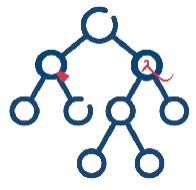
\includegraphics[height=1.0cm]{msca_logo.png}}%
    \end{center}

    \vspace{0.6cm}

    % Main title with Q logos on sides (with clickable links)
    \begin{center}
        \begin{minipage}{0.1\textwidth}
            \centering
            \href{https://quantlet.com}{
\includegraphics[height=1.1cm]{ql_logo.png}}
        \end{minipage}%
        \begin{minipage}{0.78\textwidth}
            \centering
            {\LARGE\bfseries\usebeamercolor[fg]{title}\inserttitle}

            \vspace{0.3cm}

            {\usebeamerfont{subtitle}\usebeamercolor[fg]{title}\insertsubtitle}
        \end{minipage}%
        \begin{minipage}{0.1\textwidth}
            \centering
            \href{https://quantinar.com}{
\includegraphics[height=1.1cm]{qr_logo.png}}
        \end{minipage}
    \end{center}

    \vspace{0.6cm}

    % Authors (left aligned)
    \hspace{0.5cm}{\usebeamerfont{author}\insertauthor}

    \vspace{0.3cm}

    % Institute/Affiliations (left aligned)
    \hspace{0.5cm}\begin{minipage}[t]{0.9\textwidth}
        \raggedright\small\insertinstitute
    \end{minipage}
}

%=============================================================================
% THEOREM ENVIRONMENTS
%=============================================================================
\theoremstyle{definition}
\setbeamertemplate{theorems}[numbered]
\ifdefined\sfmlang
\newtheorem{defn}{Definiție}
\newtheorem{thm}{Teoremă}
\newtheorem{prop}{Propoziție}
\newtheorem{rmk}{Observație}
\else
\newtheorem{defn}{Definition}
\newtheorem{thm}{Theorem}
\newtheorem{prop}{Proposition}
\newtheorem{rmk}{Remark}
\fi

%=============================================================================
% CENTRED MINIPAGE (no extra vertical space)
%=============================================================================
\newenvironment{cminipage}[1]{%
    \par\noindent\hfill\begin{minipage}{#1}\ignorespaces
}{%
    \end{minipage}\hfill\null\par
}

%=============================================================================
% CUSTOM COMMANDS
%=============================================================================
\newcommand{\E}{\mathbb{E}}
\newcommand{\Var}{\text{Var}}
\newcommand{\Cov}{\text{Cov}}
\newcommand{\Corr}{\text{Corr}}
\newcommand{\R}{\mathbb{R}}
\newcommand{\N}{\mathbb{N}}
\newcommand{\Z}{\mathbb{Z}}
\newcommand{\B}{\mathbf{B}}
\newcommand{\imark}{\textcolor{MainBlue}{\textbullet}}
\newcommand{\RMSE}{\text{RMSE}}
\newcommand{\MAE}{\text{MAE}}
\newcommand{\MAPE}{\text{MAPE}}

 se definește
%   \newcommand{\coursename}{Statistics of Financial Markets}      (EN)
%   \newcommand{\coursename}{Statistica piețelor financiare}       (RO)  și  \def\sfmlang{ro}
% Fișierele .tex se află în EN/Courses, EN/Seminars, RO/Cursuri, RO/Seminarii (două niveluri sub rădăcină).
% Deck-urile sînt generate de latex/build_chapterN.py / build_seminarN.py (vezi latex/sfm_build.py).

\documentclass[9pt, aspectratio=169, t]{beamer}
\providecommand{\coursename}{Statistics of Financial Markets}

% Ensure content fits on slides
\setbeamersize{text margin left=8mm, text margin right=8mm}

%=============================================================================
% THEME AND STYLE CONFIGURATION
%=============================================================================
\usetheme{default}
% Using default theme for clean header/footer control

% Color Palette (matching Redispatch PDF)
\definecolor{MainBlue}{RGB}{26, 58, 110}
\definecolor{AccentBlue}{RGB}{26, 58, 110}
\definecolor{IDAred}{RGB}{205, 0, 0}
\definecolor{DarkGray}{RGB}{51, 51, 51}
\definecolor{MediumGray}{RGB}{128, 128, 128}
\definecolor{LightGray}{RGB}{248, 248, 248}
\definecolor{VeryLightGray}{RGB}{235, 235, 235}
\definecolor{KeynoteGray}{RGB}{218, 218, 218}
\definecolor{SectionGray}{RGB}{120, 120, 120}
\definecolor{FooterGray}{RGB}{100, 100, 100}
\definecolor{Crimson}{RGB}{220, 53, 69}
\definecolor{Forest}{RGB}{46, 125, 50}
\definecolor{Amber}{RGB}{181, 133, 63}
\definecolor{Orange}{RGB}{230, 126, 34}
\definecolor{Purple}{RGB}{142, 68, 173}

% Gradient background (exact Keynote 315° gradient: white to RGB 218,218,218)
\setbeamertemplate{background}{%
    \begin{tikzpicture}[remember picture, overlay]
        \shade[shading=axis, shading angle=315,
        top color=white, bottom color=KeynoteGray]
        (current page.south west) rectangle (current page.north east);
    \end{tikzpicture}%
}
% Fallback solid color for compatibility
\setbeamercolor{background canvas}{bg=}

\setbeamercolor{palette primary}{bg=MainBlue, fg=white}
\setbeamercolor{palette secondary}{bg=MainBlue!85, fg=white}
\setbeamercolor{palette tertiary}{bg=MainBlue!70, fg=white}
\setbeamercolor{structure}{fg=MainBlue}
\setbeamercolor{title}{fg=IDAred}
\setbeamercolor{frametitle}{fg=IDAred, bg=}
\setbeamercolor{block title}{bg=MainBlue, fg=white}
\setbeamercolor{block body}{bg=VeryLightGray, fg=DarkGray}
\setbeamercolor{block title alerted}{bg=Crimson, fg=white}
\setbeamercolor{block body alerted}{bg=Crimson!8, fg=DarkGray}
\setbeamercolor{block title example}{bg=Forest, fg=white}
\setbeamercolor{block body example}{bg=Forest!8, fg=DarkGray}
\setbeamercolor{item}{fg=MainBlue}

% Footer colors (override Madrid theme blue)
\setbeamercolor{author in head/foot}{fg=FooterGray, bg=}
\setbeamercolor{title in head/foot}{fg=FooterGray, bg=}
\setbeamercolor{date in head/foot}{fg=FooterGray, bg=}
\setbeamercolor{section in head/foot}{fg=FooterGray, bg=}
\setbeamercolor{subsection in head/foot}{fg=FooterGray, bg=}

% Bullet styles (apply everywhere including blocks)
\setbeamertemplate{itemize item}{\color{MainBlue}$\boxdot$}
\setbeamertemplate{itemize subitem}{\color{MainBlue}$\blacktriangleright$}
\setbeamertemplate{itemize subsubitem}{\color{MainBlue}\tiny$\bullet$}
\setbeamertemplate{itemize/enumerate body begin}{\normalsize}
\setbeamertemplate{itemize/enumerate subbody begin}{\normalsize}

% Item spacing - compact style
\setlength{\leftmargini}{10pt}       % Level 1: minimal indent
\setlength{\leftmarginii}{10pt}      % Level 2: minimal additional indent
% Compact list spacing (zero extra space before/after lists in blocks)
\makeatletter
\def\@listi{\leftmargin\leftmargini \topsep 0pt \parsep 0pt \itemsep 0pt}
\def\@listii{\leftmargin\leftmarginii \topsep 0pt \parsep 0pt \itemsep 0pt}
\makeatother

\setbeamertemplate{navigation symbols}{}

%=============================================================================
% CUSTOM HEADLINE
%=============================================================================
\setbeamertemplate{headline}{%
    \vskip10pt%
    \hbox to \paperwidth{%
        \hskip0.5cm%
        {\small\color{FooterGray}\renewcommand{\hyperlink}[2]{##2}\insertsectionhead}%
        \hfill%
        \textcolor{FooterGray}{\small\insertframenumber}%
        \hskip0.5cm%
    }%
    \vskip4pt%
    {\color{FooterGray}\hrule height 0.4pt}%
}

%=============================================================================
% CUSTOM FOOTER
%=============================================================================
\usepackage{fontawesome5}

\setbeamertemplate{footline}{%
    {\color{FooterGray}\hrule height 0.4pt}%
    \vskip4pt%
    \hbox to \paperwidth{%
        \hskip0.5cm%
        \textcolor{FooterGray}{\small\coursename}%
        \hfill%
        \raisebox{-0.1em}{%
            \begin{tikzpicture}[x=0.08em, y=0.08em, line width=0.4pt]
                \draw[FooterGray] (0,3) -- (1,4) -- (2,3.5) -- (3,5) -- (4,4) -- (5,6) -- (6,5.5) -- (7,4) -- (8,5) -- (9,7) -- (10,6) -- (11,5) -- (12,6.5) -- (13,8) -- (14,7) -- (15,6) -- (16,7.5) -- (17,9) -- (18,8) -- (19,7) -- (20,8.5) -- (21,10) -- (22,9) -- (23,8) -- (24,9.5);
            \end{tikzpicture}%
        }%
        \hskip0.5cm%
    }%
    \vskip6pt%
}

%=============================================================================
% PACKAGES
%=============================================================================
\usepackage[utf8]{inputenc}
\DeclareUnicodeCharacter{03B1}{\ensuremath{\alpha}}
\usepackage[T1]{fontenc}
\usepackage{amsmath, amssymb, amsthm}
\usepackage{mathtools}
\usepackage{bm}
\usepackage{tikz}
\usetikzlibrary{arrows.meta, positioning, shapes, calc, decorations.pathreplacing, shadings}
\usepackage{booktabs}
\usepackage{multirow}
\usepackage{array}
\usepackage{graphicx}
\usepackage{hyperref}
\usepackage{colortbl}
\usepackage{listings}
\lstset{language=Python, basicstyle=\ttfamily\scriptsize, keywordstyle=\color{MainBlue}\bfseries,
  commentstyle=\color{Forest}, stringstyle=\color{Crimson}, breaklines=true,
  frame=none, backgroundcolor=\color{VeryLightGray}, xleftmargin=2mm}
\hypersetup{colorlinks=true, linkcolor=MainBlue, urlcolor=MainBlue}
\graphicspath{{../../logos/}{../../charts/}{../../photos/}}
\usepackage{xcolor}
\hfuzz=2pt  % Suppress tiny overfull warnings (<2pt)
\vfuzz=2pt  % Suppress tiny vertical overfull warnings (<2pt)

%=============================================================================
% QUANTLET COMMANDS
%   \quantlet{<displayed name>}{<url>}       (generic, compatible with the older SFM decks)
%   \sfmquantlet{Ch_05}{SFM_ch5_garch}       -> https://github.com/danpele/SFM/tree/main/Quantlets/Ch_05/SFM_ch5_garch
%   \qlurl{<folder>} is defined per chapter by the generator (Quantlets/Ch_NN/<folder>)
%=============================================================================
\newcommand{\sfmrepo}{https://github.com/danpele/SFM}
\newcommand{\sfmqlbase}{https://github.com/danpele/SFM/tree/main/Quantlets}
\newcommand{\quantlet}[2]{%
    \hfill\href{#2}{%
        \raisebox{-0.15em}{
\includegraphics[height=0.7em]{ql_logo.png}}%
        \textcolor{MainBlue}{\tiny\ #1}%
    }%
}
\newcommand{\sfmquantlet}[2]{\quantlet{\detokenize{#2}}{\sfmqlbase/#1/#2}}

%=============================================================================
% NOTEBOOKS (Google Colab)
%   \colaburl{notebooks/EN/chapter5_seminar_notebook.ipynb} -> the Colab link of a file in the SFM repo
%   \nb: the chapter notebook (each seminar deck redefines it with \renewcommand)
%=============================================================================
\newcommand{\colaburl}[1]{https://colab.research.google.com/github/danpele/SFM/blob/main/#1}
\newcommand{\nb}{https://colab.research.google.com/github/danpele/SFM/tree/main/notebooks/EN}
\newcommand{\nbname}{notebooks/EN}

%=============================================================================
% SLIDE HELPERS (used by the generators; the same as in MFM)
%=============================================================================
% local font size for list bodies (the preamble forces \normalsize)
\newcommand{\itemsize}[1]{\setbeamertemplate{itemize/enumerate body begin}{#1}\setbeamertemplate{itemize/enumerate subbody begin}{#1}}
\newcommand{\intitle}[1]{{\hypersetup{urlcolor=white}#1}}   % white links inside coloured title bars
\newcommand{\imgcap}[1]{{\scriptsize #1}\\[0.5mm]}          % caption under a photo
\newcommand{\imgcredit}[2]{{\tiny\color{FooterGray}\href{#1}{#2}}}   % image credit: source URL, author/licence
\newcommand{\aiprompt}[1]{{\ttfamily\color{MainBlue}#1}}     % a prompt to an AI assistant

%=============================================================================
% SEMINARS: student version by default; the instructor wrapper *_solutions.tex sets \solutionstrue
%=============================================================================
\makeatletter\@ifundefined{ifsolutions}{\expandafter\newif\csname ifsolutions\endcsname}{}\makeatother
\newcommand{\solonly}[1]{\ifsolutions #1\fi}
\newcommand{\propsub}{\ifsolutions\else\framesubtitle{\ifdefined\sfmlang Rezolvarea se discută la seminar\else Solution discussed in class\fi}\fi}

%=============================================================================
% APPENDIX AND CHAPTER LINKS (latex/appendix_links.py writes the calls; it also re-declares these
% macros before \begin{document}, so the decks compile with or without this preamble block)
%=============================================================================
\providecommand{\sfmapplink}[3]{\hypertarget{#2}{}\hyperlink{#1}{\beamergotobutton{#3}}}
\providecommand{\sfmappback}[2]{\begin{tikzpicture}[remember picture,overlay]\node[anchor=south east] at ([xshift=-3mm,yshift=7mm]current page.south east){\hyperlink{#1}{\beamerreturnbutton{#2}}};\end{tikzpicture}}
\providecommand{\sfmchlink}[2]{\href{#1}{#2}}
\providecommand{\sfmchlinkt}[2]{\href{#1}{\usebeamercolor[fg]{frametitle}#2}}

%=============================================================================
% QUANTINAR COMMAND: link către un curs Quantinar (subiecte avansate)
%=============================================================================
\newcommand{\quantinar}[2]{%
    \href{#2}{%
        \raisebox{-0.15em}{
\includegraphics[height=0.8em]{qr_logo.png}}%
        \textcolor{MainBlue}{\scriptsize\ #1}%
    }%
}

%=============================================================================
% CUSTOM TITLE PAGE
%=============================================================================
\defbeamertemplate*{title page}{hybrid}[1][]
{
    \vspace{0.2cm}
    % Logos row - top header (with clickable links)
    \begin{center}
        \href{https://www.ase.ro}{
\includegraphics[height=1.0cm]{ase_logo.png}}\hspace{0.3cm}%
        \href{https://theida.net}{
\includegraphics[height=1.0cm]{ida_logo.png}}\hspace{0.3cm}%
        \href{https://blockchain-research-center.com}{
\includegraphics[height=1.0cm]{brc_logo.png}}\hspace{0.3cm}%
        \href{https://www.ai4efin.ase.ro}{
\includegraphics[height=1.0cm]{ai4efin_logo.png}}\hspace{0.3cm}%
        \href{https://ipe.ro/new}{
\includegraphics[height=1.0cm]{acad_logo.png}}\hspace{0.3cm}%
        \href{https://www.digital-finance-msca.com}{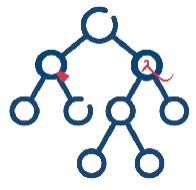
\includegraphics[height=1.0cm]{msca_logo.png}}%
    \end{center}

    \vspace{0.6cm}

    % Main title with Q logos on sides (with clickable links)
    \begin{center}
        \begin{minipage}{0.1\textwidth}
            \centering
            \href{https://quantlet.com}{
\includegraphics[height=1.1cm]{ql_logo.png}}
        \end{minipage}%
        \begin{minipage}{0.78\textwidth}
            \centering
            {\LARGE\bfseries\usebeamercolor[fg]{title}\inserttitle}

            \vspace{0.3cm}

            {\usebeamerfont{subtitle}\usebeamercolor[fg]{title}\insertsubtitle}
        \end{minipage}%
        \begin{minipage}{0.1\textwidth}
            \centering
            \href{https://quantinar.com}{
\includegraphics[height=1.1cm]{qr_logo.png}}
        \end{minipage}
    \end{center}

    \vspace{0.6cm}

    % Authors (left aligned)
    \hspace{0.5cm}{\usebeamerfont{author}\insertauthor}

    \vspace{0.3cm}

    % Institute/Affiliations (left aligned)
    \hspace{0.5cm}\begin{minipage}[t]{0.9\textwidth}
        \raggedright\small\insertinstitute
    \end{minipage}
}

%=============================================================================
% THEOREM ENVIRONMENTS
%=============================================================================
\theoremstyle{definition}
\setbeamertemplate{theorems}[numbered]
\ifdefined\sfmlang
\newtheorem{defn}{Definiție}
\newtheorem{thm}{Teoremă}
\newtheorem{prop}{Propoziție}
\newtheorem{rmk}{Observație}
\else
\newtheorem{defn}{Definition}
\newtheorem{thm}{Theorem}
\newtheorem{prop}{Proposition}
\newtheorem{rmk}{Remark}
\fi

%=============================================================================
% CENTRED MINIPAGE (no extra vertical space)
%=============================================================================
\newenvironment{cminipage}[1]{%
    \par\noindent\hfill\begin{minipage}{#1}\ignorespaces
}{%
    \end{minipage}\hfill\null\par
}

%=============================================================================
% CUSTOM COMMANDS
%=============================================================================
\newcommand{\E}{\mathbb{E}}
\newcommand{\Var}{\text{Var}}
\newcommand{\Cov}{\text{Cov}}
\newcommand{\Corr}{\text{Corr}}
\newcommand{\R}{\mathbb{R}}
\newcommand{\N}{\mathbb{N}}
\newcommand{\Z}{\mathbb{Z}}
\newcommand{\B}{\mathbf{B}}
\newcommand{\imark}{\textcolor{MainBlue}{\textbullet}}
\newcommand{\RMSE}{\text{RMSE}}
\newcommand{\MAE}{\text{MAE}}
\newcommand{\MAPE}{\text{MAPE}}

 se definește
%   \newcommand{\coursename}{Statistics of Financial Markets}      (EN)
%   \newcommand{\coursename}{Statistica piețelor financiare}       (RO)  și  \def\sfmlang{ro}
% Fișierele .tex se află în EN/Courses, EN/Seminars, RO/Cursuri, RO/Seminarii (două niveluri sub rădăcină).
% Deck-urile sînt generate de latex/build_chapterN.py / build_seminarN.py (vezi latex/sfm_build.py).

\documentclass[9pt, aspectratio=169, t]{beamer}
\providecommand{\coursename}{Statistics of Financial Markets}

% Ensure content fits on slides
\setbeamersize{text margin left=8mm, text margin right=8mm}

%=============================================================================
% THEME AND STYLE CONFIGURATION
%=============================================================================
\usetheme{default}
% Using default theme for clean header/footer control

% Color Palette (matching Redispatch PDF)
\definecolor{MainBlue}{RGB}{26, 58, 110}
\definecolor{AccentBlue}{RGB}{26, 58, 110}
\definecolor{IDAred}{RGB}{205, 0, 0}
\definecolor{DarkGray}{RGB}{51, 51, 51}
\definecolor{MediumGray}{RGB}{128, 128, 128}
\definecolor{LightGray}{RGB}{248, 248, 248}
\definecolor{VeryLightGray}{RGB}{235, 235, 235}
\definecolor{KeynoteGray}{RGB}{218, 218, 218}
\definecolor{SectionGray}{RGB}{120, 120, 120}
\definecolor{FooterGray}{RGB}{100, 100, 100}
\definecolor{Crimson}{RGB}{220, 53, 69}
\definecolor{Forest}{RGB}{46, 125, 50}
\definecolor{Amber}{RGB}{181, 133, 63}
\definecolor{Orange}{RGB}{230, 126, 34}
\definecolor{Purple}{RGB}{142, 68, 173}

% Gradient background (exact Keynote 315° gradient: white to RGB 218,218,218)
\setbeamertemplate{background}{%
    \begin{tikzpicture}[remember picture, overlay]
        \shade[shading=axis, shading angle=315,
        top color=white, bottom color=KeynoteGray]
        (current page.south west) rectangle (current page.north east);
    \end{tikzpicture}%
}
% Fallback solid color for compatibility
\setbeamercolor{background canvas}{bg=}

\setbeamercolor{palette primary}{bg=MainBlue, fg=white}
\setbeamercolor{palette secondary}{bg=MainBlue!85, fg=white}
\setbeamercolor{palette tertiary}{bg=MainBlue!70, fg=white}
\setbeamercolor{structure}{fg=MainBlue}
\setbeamercolor{title}{fg=IDAred}
\setbeamercolor{frametitle}{fg=IDAred, bg=}
\setbeamercolor{block title}{bg=MainBlue, fg=white}
\setbeamercolor{block body}{bg=VeryLightGray, fg=DarkGray}
\setbeamercolor{block title alerted}{bg=Crimson, fg=white}
\setbeamercolor{block body alerted}{bg=Crimson!8, fg=DarkGray}
\setbeamercolor{block title example}{bg=Forest, fg=white}
\setbeamercolor{block body example}{bg=Forest!8, fg=DarkGray}
\setbeamercolor{item}{fg=MainBlue}

% Footer colors (override Madrid theme blue)
\setbeamercolor{author in head/foot}{fg=FooterGray, bg=}
\setbeamercolor{title in head/foot}{fg=FooterGray, bg=}
\setbeamercolor{date in head/foot}{fg=FooterGray, bg=}
\setbeamercolor{section in head/foot}{fg=FooterGray, bg=}
\setbeamercolor{subsection in head/foot}{fg=FooterGray, bg=}

% Bullet styles (apply everywhere including blocks)
\setbeamertemplate{itemize item}{\color{MainBlue}$\boxdot$}
\setbeamertemplate{itemize subitem}{\color{MainBlue}$\blacktriangleright$}
\setbeamertemplate{itemize subsubitem}{\color{MainBlue}\tiny$\bullet$}
\setbeamertemplate{itemize/enumerate body begin}{\normalsize}
\setbeamertemplate{itemize/enumerate subbody begin}{\normalsize}

% Item spacing - compact style
\setlength{\leftmargini}{10pt}       % Level 1: minimal indent
\setlength{\leftmarginii}{10pt}      % Level 2: minimal additional indent
% Compact list spacing (zero extra space before/after lists in blocks)
\makeatletter
\def\@listi{\leftmargin\leftmargini \topsep 0pt \parsep 0pt \itemsep 0pt}
\def\@listii{\leftmargin\leftmarginii \topsep 0pt \parsep 0pt \itemsep 0pt}
\makeatother

\setbeamertemplate{navigation symbols}{}

%=============================================================================
% CUSTOM HEADLINE
%=============================================================================
\setbeamertemplate{headline}{%
    \vskip10pt%
    \hbox to \paperwidth{%
        \hskip0.5cm%
        {\small\color{FooterGray}\renewcommand{\hyperlink}[2]{##2}\insertsectionhead}%
        \hfill%
        \textcolor{FooterGray}{\small\insertframenumber}%
        \hskip0.5cm%
    }%
    \vskip4pt%
    {\color{FooterGray}\hrule height 0.4pt}%
}

%=============================================================================
% CUSTOM FOOTER
%=============================================================================
\usepackage{fontawesome5}

\setbeamertemplate{footline}{%
    {\color{FooterGray}\hrule height 0.4pt}%
    \vskip4pt%
    \hbox to \paperwidth{%
        \hskip0.5cm%
        \textcolor{FooterGray}{\small\coursename}%
        \hfill%
        \raisebox{-0.1em}{%
            \begin{tikzpicture}[x=0.08em, y=0.08em, line width=0.4pt]
                \draw[FooterGray] (0,3) -- (1,4) -- (2,3.5) -- (3,5) -- (4,4) -- (5,6) -- (6,5.5) -- (7,4) -- (8,5) -- (9,7) -- (10,6) -- (11,5) -- (12,6.5) -- (13,8) -- (14,7) -- (15,6) -- (16,7.5) -- (17,9) -- (18,8) -- (19,7) -- (20,8.5) -- (21,10) -- (22,9) -- (23,8) -- (24,9.5);
            \end{tikzpicture}%
        }%
        \hskip0.5cm%
    }%
    \vskip6pt%
}

%=============================================================================
% PACKAGES
%=============================================================================
\usepackage[utf8]{inputenc}
\DeclareUnicodeCharacter{03B1}{\ensuremath{\alpha}}
\usepackage[T1]{fontenc}
\usepackage{amsmath, amssymb, amsthm}
\usepackage{mathtools}
\usepackage{bm}
\usepackage{tikz}
\usetikzlibrary{arrows.meta, positioning, shapes, calc, decorations.pathreplacing, shadings}
\usepackage{booktabs}
\usepackage{multirow}
\usepackage{array}
\usepackage{graphicx}
\usepackage{hyperref}
\usepackage{colortbl}
\usepackage{listings}
\lstset{language=Python, basicstyle=\ttfamily\scriptsize, keywordstyle=\color{MainBlue}\bfseries,
  commentstyle=\color{Forest}, stringstyle=\color{Crimson}, breaklines=true,
  frame=none, backgroundcolor=\color{VeryLightGray}, xleftmargin=2mm}
\hypersetup{colorlinks=true, linkcolor=MainBlue, urlcolor=MainBlue}
\graphicspath{{../../logos/}{../../charts/}{../../photos/}}
\usepackage{xcolor}
\hfuzz=2pt  % Suppress tiny overfull warnings (<2pt)
\vfuzz=2pt  % Suppress tiny vertical overfull warnings (<2pt)

%=============================================================================
% QUANTLET COMMANDS
%   \quantlet{<displayed name>}{<url>}       (generic, compatible with the older SFM decks)
%   \sfmquantlet{Ch_05}{SFM_ch5_garch}       -> https://github.com/danpele/SFM/tree/main/Quantlets/Ch_05/SFM_ch5_garch
%   \qlurl{<folder>} is defined per chapter by the generator (Quantlets/Ch_NN/<folder>)
%=============================================================================
\newcommand{\sfmrepo}{https://github.com/danpele/SFM}
\newcommand{\sfmqlbase}{https://github.com/danpele/SFM/tree/main/Quantlets}
\newcommand{\quantlet}[2]{%
    \hfill\href{#2}{%
        \raisebox{-0.15em}{
\includegraphics[height=0.7em]{ql_logo.png}}%
        \textcolor{MainBlue}{\tiny\ #1}%
    }%
}
\newcommand{\sfmquantlet}[2]{\quantlet{\detokenize{#2}}{\sfmqlbase/#1/#2}}

%=============================================================================
% NOTEBOOKS (Google Colab)
%   \colaburl{notebooks/EN/chapter5_seminar_notebook.ipynb} -> the Colab link of a file in the SFM repo
%   \nb: the chapter notebook (each seminar deck redefines it with \renewcommand)
%=============================================================================
\newcommand{\colaburl}[1]{https://colab.research.google.com/github/danpele/SFM/blob/main/#1}
\newcommand{\nb}{https://colab.research.google.com/github/danpele/SFM/tree/main/notebooks/EN}
\newcommand{\nbname}{notebooks/EN}

%=============================================================================
% SLIDE HELPERS (used by the generators; the same as in MFM)
%=============================================================================
% local font size for list bodies (the preamble forces \normalsize)
\newcommand{\itemsize}[1]{\setbeamertemplate{itemize/enumerate body begin}{#1}\setbeamertemplate{itemize/enumerate subbody begin}{#1}}
\newcommand{\intitle}[1]{{\hypersetup{urlcolor=white}#1}}   % white links inside coloured title bars
\newcommand{\imgcap}[1]{{\scriptsize #1}\\[0.5mm]}          % caption under a photo
\newcommand{\imgcredit}[2]{{\tiny\color{FooterGray}\href{#1}{#2}}}   % image credit: source URL, author/licence
\newcommand{\aiprompt}[1]{{\ttfamily\color{MainBlue}#1}}     % a prompt to an AI assistant

%=============================================================================
% SEMINARS: student version by default; the instructor wrapper *_solutions.tex sets \solutionstrue
%=============================================================================
\makeatletter\@ifundefined{ifsolutions}{\expandafter\newif\csname ifsolutions\endcsname}{}\makeatother
\newcommand{\solonly}[1]{\ifsolutions #1\fi}
\newcommand{\propsub}{\ifsolutions\else\framesubtitle{\ifdefined\sfmlang Rezolvarea se discută la seminar\else Solution discussed in class\fi}\fi}

%=============================================================================
% APPENDIX AND CHAPTER LINKS (latex/appendix_links.py writes the calls; it also re-declares these
% macros before \begin{document}, so the decks compile with or without this preamble block)
%=============================================================================
\providecommand{\sfmapplink}[3]{\hypertarget{#2}{}\hyperlink{#1}{\beamergotobutton{#3}}}
\providecommand{\sfmappback}[2]{\begin{tikzpicture}[remember picture,overlay]\node[anchor=south east] at ([xshift=-3mm,yshift=7mm]current page.south east){\hyperlink{#1}{\beamerreturnbutton{#2}}};\end{tikzpicture}}
\providecommand{\sfmchlink}[2]{\href{#1}{#2}}
\providecommand{\sfmchlinkt}[2]{\href{#1}{\usebeamercolor[fg]{frametitle}#2}}

%=============================================================================
% QUANTINAR COMMAND: link către un curs Quantinar (subiecte avansate)
%=============================================================================
\newcommand{\quantinar}[2]{%
    \href{#2}{%
        \raisebox{-0.15em}{
\includegraphics[height=0.8em]{qr_logo.png}}%
        \textcolor{MainBlue}{\scriptsize\ #1}%
    }%
}

%=============================================================================
% CUSTOM TITLE PAGE
%=============================================================================
\defbeamertemplate*{title page}{hybrid}[1][]
{
    \vspace{0.2cm}
    % Logos row - top header (with clickable links)
    \begin{center}
        \href{https://www.ase.ro}{
\includegraphics[height=1.0cm]{ase_logo.png}}\hspace{0.3cm}%
        \href{https://theida.net}{
\includegraphics[height=1.0cm]{ida_logo.png}}\hspace{0.3cm}%
        \href{https://blockchain-research-center.com}{
\includegraphics[height=1.0cm]{brc_logo.png}}\hspace{0.3cm}%
        \href{https://www.ai4efin.ase.ro}{
\includegraphics[height=1.0cm]{ai4efin_logo.png}}\hspace{0.3cm}%
        \href{https://ipe.ro/new}{
\includegraphics[height=1.0cm]{acad_logo.png}}\hspace{0.3cm}%
        \href{https://www.digital-finance-msca.com}{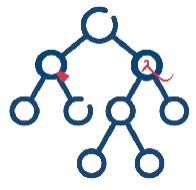
\includegraphics[height=1.0cm]{msca_logo.png}}%
    \end{center}

    \vspace{0.6cm}

    % Main title with Q logos on sides (with clickable links)
    \begin{center}
        \begin{minipage}{0.1\textwidth}
            \centering
            \href{https://quantlet.com}{
\includegraphics[height=1.1cm]{ql_logo.png}}
        \end{minipage}%
        \begin{minipage}{0.78\textwidth}
            \centering
            {\LARGE\bfseries\usebeamercolor[fg]{title}\inserttitle}

            \vspace{0.3cm}

            {\usebeamerfont{subtitle}\usebeamercolor[fg]{title}\insertsubtitle}
        \end{minipage}%
        \begin{minipage}{0.1\textwidth}
            \centering
            \href{https://quantinar.com}{
\includegraphics[height=1.1cm]{qr_logo.png}}
        \end{minipage}
    \end{center}

    \vspace{0.6cm}

    % Authors (left aligned)
    \hspace{0.5cm}{\usebeamerfont{author}\insertauthor}

    \vspace{0.3cm}

    % Institute/Affiliations (left aligned)
    \hspace{0.5cm}\begin{minipage}[t]{0.9\textwidth}
        \raggedright\small\insertinstitute
    \end{minipage}
}

%=============================================================================
% THEOREM ENVIRONMENTS
%=============================================================================
\theoremstyle{definition}
\setbeamertemplate{theorems}[numbered]
\ifdefined\sfmlang
\newtheorem{defn}{Definiție}
\newtheorem{thm}{Teoremă}
\newtheorem{prop}{Propoziție}
\newtheorem{rmk}{Observație}
\else
\newtheorem{defn}{Definition}
\newtheorem{thm}{Theorem}
\newtheorem{prop}{Proposition}
\newtheorem{rmk}{Remark}
\fi

%=============================================================================
% CENTRED MINIPAGE (no extra vertical space)
%=============================================================================
\newenvironment{cminipage}[1]{%
    \par\noindent\hfill\begin{minipage}{#1}\ignorespaces
}{%
    \end{minipage}\hfill\null\par
}

%=============================================================================
% CUSTOM COMMANDS
%=============================================================================
\newcommand{\E}{\mathbb{E}}
\newcommand{\Var}{\text{Var}}
\newcommand{\Cov}{\text{Cov}}
\newcommand{\Corr}{\text{Corr}}
\newcommand{\R}{\mathbb{R}}
\newcommand{\N}{\mathbb{N}}
\newcommand{\Z}{\mathbb{Z}}
\newcommand{\B}{\mathbf{B}}
\newcommand{\imark}{\textcolor{MainBlue}{\textbullet}}
\newcommand{\RMSE}{\text{RMSE}}
\newcommand{\MAE}{\text{MAE}}
\newcommand{\MAPE}{\text{MAPE}}



\newcommand{\qlurl}[1]{https://github.com/danpele/SFM/tree/main/Quantlets/Ch_07/#1}

% Clickable citations (DOIs verified via Crossref)

\newcommand{\refFamaA}{\href{https://doi.org/10.1111/j.1540-6261.1970.tb00518.x}{Fama (1970)}}
\newcommand{\refFamaB}{\href{https://doi.org/10.1111/j.1540-6261.1991.tb04636.x}{Fama (1991)}}
\newcommand{\refFamaC}{\href{https://doi.org/10.1086/294743}{Fama (1965)}}
\newcommand{\refSamuelson}{\href{https://doi.org/10.1142/9789814566926_0002}{Samuelson (1965)}}
\newcommand{\refBachelier}{\href{https://doi.org/10.24033/asens.476}{Bachelier (1900)}}
\newcommand{\refKendall}{\href{https://doi.org/10.2307/2980947}{Kendall (1953)}}
\newcommand{\refRoberts}{\href{https://doi.org/10.1111/j.1540-6261.1959.tb00481.x}{Roberts (1959)}}
\newcommand{\refLM}{\href{https://doi.org/10.1093/rfs/1.1.41}{Lo \& MacKinlay (1988)}}
\newcommand{\refLo}{\href{https://doi.org/10.3905/jpm.2004.442611}{Lo (2004)}}
\newcommand{\refLoBook}{\href{https://doi.org/10.1515/9781400887767}{Lo (2017)}}
\newcommand{\refCLM}{\href{https://doi.org/10.1515/9781400830213}{Campbell, Lo \& MacKinlay (1997)}}
\newcommand{\refCD}{\href{https://doi.org/10.1016/0304-4076(93)90051-6}{Chow \& Denning (1993)}}
\newcommand{\refChoi}{\href{https://doi.org/10.1002/(SICI)1099-1255(199905/06)14:3<293::AID-JAE503>3.0.CO;2-5}{Choi (1999)}}
\newcommand{\refKimB}{\href{https://doi.org/10.1016/j.frl.2009.04.003}{Kim (2009)}}
\newcommand{\refAndrews}{\href{https://doi.org/10.2307/2938229}{Andrews (1991)}}
\newcommand{\refLjung}{\href{https://doi.org/10.1093/biomet/65.2.297}{Ljung \& Box (1978)}}
\newcommand{\refBP}{\href{https://doi.org/10.1080/01621459.1970.10481180}{Box \& Pierce (1970)}}
\newcommand{\refWW}{\href{https://doi.org/10.1214/aoms/1177731909}{Wald \& Wolfowitz (1940)}}
\newcommand{\refEL}{\href{https://doi.org/10.1016/j.jeconom.2009.03.001}{Escanciano \& Lobato (2009)}}
\newcommand{\refDF}{\href{https://doi.org/10.1080/01621459.1979.10482531}{Dickey \& Fuller (1979)}}
\newcommand{\refSD}{\href{https://doi.org/10.1093/biomet/71.3.599}{Said \& Dickey (1984)}}
\newcommand{\refPP}{\href{https://doi.org/10.1093/biomet/75.2.335}{Phillips \& Perron (1988)}}
\newcommand{\refKPSS}{\href{https://doi.org/10.1016/0304-4076(92)90104-Y}{Kwiatkowski et al.\ (1992)}}
\newcommand{\refMacKinnon}{\href{https://doi.org/10.1002/(SICI)1099-1255(199611)11:6<601::AID-JAE417>3.0.CO;2-T}{MacKinnon (1996)}}
\newcommand{\refNW}{\href{https://doi.org/10.2307/1913610}{Newey \& West (1987)}}
\newcommand{\refGN}{\href{https://doi.org/10.1016/0304-4076(74)90034-7}{Granger \& Newbold (1974)}}
\newcommand{\refUrquhart}{\href{https://doi.org/10.1016/j.econlet.2016.09.019}{Urquhart (2016)}}
\newcommand{\refUM}{\href{https://doi.org/10.1016/j.irfa.2016.06.011}{Urquhart \& McGroarty (2016)}}
\newcommand{\refKSL}{\href{https://doi.org/10.1016/j.jempfin.2011.08.002}{Kim, Shamsuddin \& Lim (2011)}}
\newcommand{\refLB}{\href{https://doi.org/10.1111/j.1467-6419.2009.00611.x}{Lim \& Brooks (2011)}}
\newcommand{\refGS}{\href{https://ideas.repec.org/a/aea/aecrev/v70y1980i3p393-408.html}{Grossman \& Stiglitz (1980)}}
\newcommand{\refFrench}{\href{https://doi.org/10.1016/0304-405X(80)90021-5}{French (1980)}}
\newcommand{\refRK}{\href{https://doi.org/10.1016/0304-405X(76)90028-3}{Rozeff \& Kinney (1976)}}
\newcommand{\refAriel}{\href{https://doi.org/10.1016/0304-405X(87)90066-3}{Ariel (1987)}}
\newcommand{\refMP}{\href{https://doi.org/10.1111/jofi.12365}{McLean \& Pontiff (2016)}}
\newcommand{\refHLZ}{\href{https://doi.org/10.1093/rfs/hhv059}{Harvey, Liu \& Zhu (2016)}}
\newcommand{\refMacKinlay}{\href{https://ideas.repec.org/a/aea/jeclit/v35y1997i1p13-39.html}{MacKinlay (1997)}}
\newcommand{\refJensen}{\href{https://doi.org/10.1111/j.1540-6261.1968.tb00815.x}{Jensen (1968)}}
\newcommand{\refFF}{\href{https://doi.org/10.1111/j.1540-6261.2010.01598.x}{Fama \& French (2010)}}
\newcommand{\refMalkiel}{\href{https://doi.org/10.1257/089533003321164958}{Malkiel (2003)}}
\newcommand{\refFHH}{\href{https://doi.org/10.1007/978-3-030-13751-9}{Franke, Härdle \& Hafner (2019)}}
\newcommand{\refBHL}{\href{https://doi.org/10.1007/978-3-642-33929-5}{Borak, Härdle \& López-Cabrera (2013)}}
\newcommand{\refTsay}{\href{https://doi.org/10.1002/9780470644560}{Tsay (2010)}}
\newcommand{\refWang}{\href{https://doi.org/10.1038/s41586-023-06221-2}{Wang et al.\ (2023)}}
\newcommand{\refPeleA}{\href{https://doi.org/10.1016/j.sbspro.2012.09.1030}{Pele \& Mazurencu-Marinescu (2012)}}
\newcommand{\refPeleB}{\href{https://doi.org/10.2139/ssrn.7157232}{Tak, Schlamp, Osterrieder \& Pele (2026)}}
\newcommand{\refPeleC}{\href{https://doi.org/10.2139/ssrn.5176758}{Lin, Găman, Wang \& Pele (2025)}}
\newcommand{\refFTSE}{\href{https://www.lseg.com/en/media-centre/press-releases/ftse-russell/2019/ftse-russell-announces-results-country-classification-review-equities-and-fixed-income}{FTSE Russell (2019)}}

\title[Statistics of Financial Markets]{Statistics of Financial Markets}
\subtitle{Chapter 7: Efficient markets, random walk and variance-ratio tests}
\author[D.T. Pele]{Daniel Traian PELE}
\institute{Bucharest University of Economic Studies\\
IDA Institute Digital Assets\\
Blockchain Research Center\\
AI4EFin Artificial Intelligence for Energy Finance\\
Romanian Academy, Institute for Economic Forecasting\\
MSCA Digital Finance}
\date{}

%=============================================================================
\providecommand{\sfmapplink}[3]{\hypertarget{#2}{}\hyperlink{#1}{\beamergotobutton{#3}}}  % APPLINKS-MACROS
\providecommand{\sfmappback}[2]{\begin{tikzpicture}[remember picture,overlay]\node[anchor=south east] at ([xshift=-3mm,yshift=7mm]current page.south east){\hyperlink{#1}{\beamerreturnbutton{#2}}};\end{tikzpicture}}  % APPLINKS-MACROS
\providecommand{\sfmchlink}[2]{\href{#1}{#2}}  % APPLINKS-MACROS
\providecommand{\sfmchlinkt}[2]{\href{#1}{\usebeamercolor[fg]{frametitle}#2}}  % APPLINKS-MACROS
\begin{document}
%=============================================================================

{
\setbeamertemplate{headline}{}
\setbeamertemplate{footline}{}
\begin{frame}[noframenumbering]
    \titlepage
\end{frame}
}
% BEGIN-ACRONYMS (generat de latex/acronyms.py; nu editati manual)
\begin{frame}{Acronyms used in this material (1/2)}
\setbeamertemplate{itemize/enumerate body begin}{\tiny}
\begin{columns}[T]
\begin{column}{0.49\textwidth}
\begin{itemize}\setlength{\itemsep}{0pt}
    \item \textbf{ACF}: Autocorrelation Function
    \item \textbf{ADF}: Augmented Dickey–Fuller (test)
    \item \textbf{AI}: Artificial Intelligence
    \item \textbf{AIC}: Akaike Information Criterion
    \item \textbf{AMH}: Adaptive Markets Hypothesis
    \item \textbf{AR}: AutoRegressive (model)
    \item \textbf{BET}: Bucharest Exchange Trading (index)
    \item \textbf{BET-TR}: BET Total Return (index)
    \item \textbf{BUX}: Budapesti Értéktőzsde index (the Budapest Stock Exchange index)
    \item \textbf{BVB}: Bursa de Valori București (the Bucharest Stock Exchange)
    \item \textbf{CAPM}: Capital Asset Pricing Model
    \item \textbf{CD}: Chow–Denning (multiple variance-ratio test)
    \item \textbf{CME}: Chicago Mercantile Exchange
\end{itemize}
\end{column}
\begin{column}{0.49\textwidth}
\begin{itemize}\setlength{\itemsep}{0pt}
    \item \textbf{COVID-19}: COronaVIrus Disease 2019
    \item \textbf{EMH}: Efficient Market Hypothesis
    \item \textbf{EODHD}: EOD Historical Data (market-data provider)
    \item \textbf{EU}: European Union
    \item \textbf{FTSE}: Financial Times Stock Exchange (FTSE Russell, index provider)
    \item \textbf{GARCH}: Generalised AutoRegressive Conditional Heteroskedasticity
    \item \textbf{GMM}: Generalized Method of Moments
    \item \textbf{KPSS}: Kwiatkowski–Phillips–Schmidt–Shin (stationarity test)
    \item \textbf{LB}: Ljung–Box (test)
    \item \textbf{MA}: Moving Average (model)
    \item \textbf{MIT}: Massachusetts Institute of Technology
    \item \textbf{OLS}: Ordinary Least Squares
    \item \textbf{PP}: Phillips–Perron (unit-root test)
\end{itemize}
\end{column}
\end{columns}
\end{frame}
\begin{frame}{Acronyms used in this material (2/2)}
\setbeamertemplate{itemize/enumerate body begin}{\tiny}
\begin{columns}[T]
\begin{column}{0.49\textwidth}
\begin{itemize}\setlength{\itemsep}{0pt}
    \item \textbf{PX}: Prague Stock Exchange index (index Burzy cenných papírů Praha)
    \item \textbf{RW1}: Random Walk 1 (i.i.d. increments)
    \item \textbf{RW2}: Random Walk 2 (independent increments)
    \item \textbf{RW3}: Random Walk 3 (uncorrelated increments)
    \item \textbf{SFE}: Statistics of Financial Markets, Exercises (Quantlet collection of the textbook)
    \item \textbf{VR}: Variance Ratio
    \item \textbf{WIG20}: Warszawski Indeks Giełdowy 20 (the Warsaw Stock Exchange index of the 20 largest companies)
\end{itemize}
\end{column}
\begin{column}{0.49\textwidth}
\end{column}
\end{columns}
\end{frame}
% END-ACRONYMS

\begin{frame}{Today's Question and Route}
\itemsize{\small}
\begin{itemize}
    \item \textbf{Question}: can yesterday's prices tell us anything about tomorrow's return?
    \begin{itemize}
        \item if yes, a simple rule could beat the market; if no, the market is efficient in the weak sense
        \item \sfmchlink{https://danpele.github.io/SFM/EN/Courses/chapter4_probability.pdf}{Chapter 4} defined the random walk and the martingale; here we test them on real prices
    \end{itemize}
    \item \textbf{Route} of the chapter
    \begin{itemize}
        \item efficient markets: three forms, the joint-hypothesis problem
        \item random walk hypotheses RW1, RW2, RW3 and the martingale
        \item white noise and the autocorrelation function; Ljung--Box and runs tests
        \item unit roots: ADF, Phillips--Perron, KPSS; prices against returns
        \item variance-ratio tests; efficiency across markets and over time; anomalies
    \end{itemize}
\end{itemize}
\end{frame}

\begin{frame}{Learning Outcomes}
\itemsize{\small}
\begin{itemize}
    \item State the three forms of market efficiency and explain why every test is a joint test
    \item Tell RW1, RW2, RW3 and the martingale apart, and say which of them volatility clustering violates
    \item Read a sample ACF with the right confidence band and compute Box--Pierce, Ljung--Box and runs statistics
    \item Run and combine ADF, Phillips--Perron and KPSS tests on prices and on returns
    \item Compute a variance ratio and its robust test, for one horizon and for several horizons together
    \item Judge, on real data, which markets look efficient, and whether this changes over time
\end{itemize}
\end{frame}

\begin{frame}{Reading and Tools}
\itemsize{\small}
\begin{itemize}
    \item Textbook: \refFHH, Ch.~11 (11.3 expectations and efficient markets, 11.5 random walk tests, 11.6 unit root tests)
    \begin{itemize}
        \item exercises with solutions: \refBHL, Ch.~11
    \end{itemize}
    \item Econometrics of predictability: \refCLM, Ch.~2 (random walks, variance ratios) and Ch.~4 (event studies)
    \item Python Quantlets of this chapter: \href{https://github.com/danpele/SFM/tree/main/Quantlets/Ch_07}{Quantlets/Ch\_07}
    \begin{itemize}
        \item ported from the SFE Quantlets SFEtimewn, SFEacfar1, SFEacfar2, SFEacfma1 and SFEacfma2
    \end{itemize}
    \item Lecture notebook: \href{\colaburl{notebooks/EN/chapter7_lecture_notebook.ipynb}}{open in Google Colab}
    \item Video course: \quantinar{Efficiency of cryptocurrency markets -- A GMM-based analysis}{https://quantinar.com/course/184/efficiency-of-cryptocurrency-markets-a-gmm-based-analysis}
\end{itemize}
\end{frame}


%=============================================================================
\section{Can Prices Be Predicted?}
%=============================================================================

\begin{frame}{Can You Beat the Market?}
\itemsize{\small}
\begin{columns}[T]
\begin{column}{0.54\textwidth}
\begin{itemize}
    \item If past prices predicted future returns, a simple rule would earn money with no risk
    \begin{itemize}
        \item traders would use the rule; their trades would move prices until the pattern disappears
    \end{itemize}
    \item The evidence on professional investors
    \begin{itemize}
        \item mutual funds, on average, did not beat a buy-and-hold portfolio after costs \refJensen
        \item few funds show skill large enough to cover their costs \refFF
    \end{itemize}
    \item A survey of the arguments for and against: \refMalkiel
\end{itemize}
\end{column}
\begin{column}{0.42\textwidth}
\centering
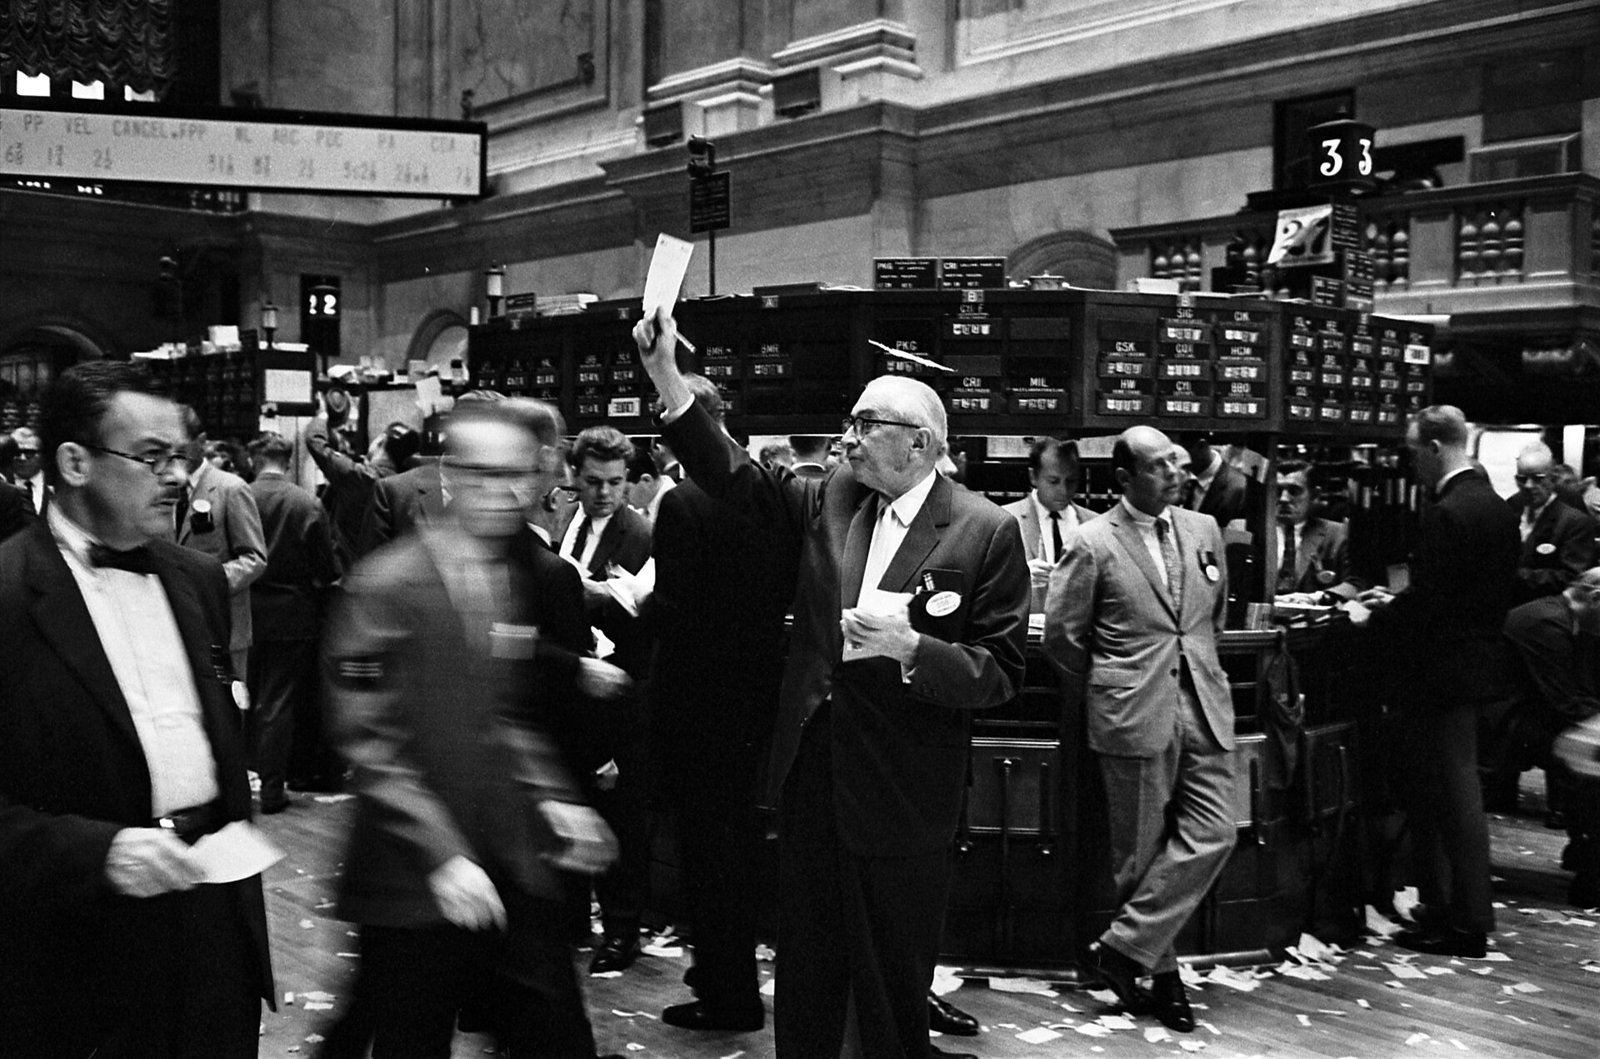
\includegraphics[height=0.36\textheight]{ch0_nyse_floor_1963.jpg}\\[1mm]
\imgcap{The trading floor of the New York Stock Exchange, 1963}
\imgcredit{https://commons.wikimedia.org/wiki/File:NY_stock_exchange_traders_floor_LC-U9-10548-6.jpg}{Photo: Thomas J. O'Halloran (1963), Library of Congress; public domain; Wikimedia Commons}
\end{column}
\end{columns}
\end{frame}

\begin{frame}{1900: Prices as a Random Walk}
\itemsize{\small}
\begin{columns}[T]
\begin{column}{0.64\textwidth}
\begin{itemize}
    \item Louis Bachelier, \textit{Théorie de la spéculation} \refBachelier
    \begin{itemize}
        \item the first mathematical model of prices: the change of a price is a sum of many small random shocks
        \item the expected gain of the speculator is zero
    \end{itemize}
    \item \refKendall: 22 British price series behave like a ``wandering'' series
    \begin{itemize}
        \item the changes from one week to the next look like independent draws
    \end{itemize}
    \item \refRoberts: simulated random walks show ``patterns'' that chartists see in real prices
\end{itemize}
\end{column}
\begin{column}{0.32\textwidth}
\centering
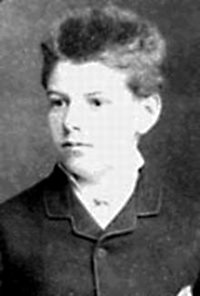
\includegraphics[height=0.42\textheight]{ch0_bachelier.jpg}\\[1mm]
\imgcap{Louis Bachelier (1870--1946)}
\imgcredit{https://commons.wikimedia.org/wiki/File:LouisBachelier.jpg}{Photo: unknown author; public domain; Wikimedia Commons}
\end{column}
\end{columns}
\end{frame}

\begin{frame}{Which One Is the S\&P 500?}
\itemsize{\footnotesize}
\begin{center}
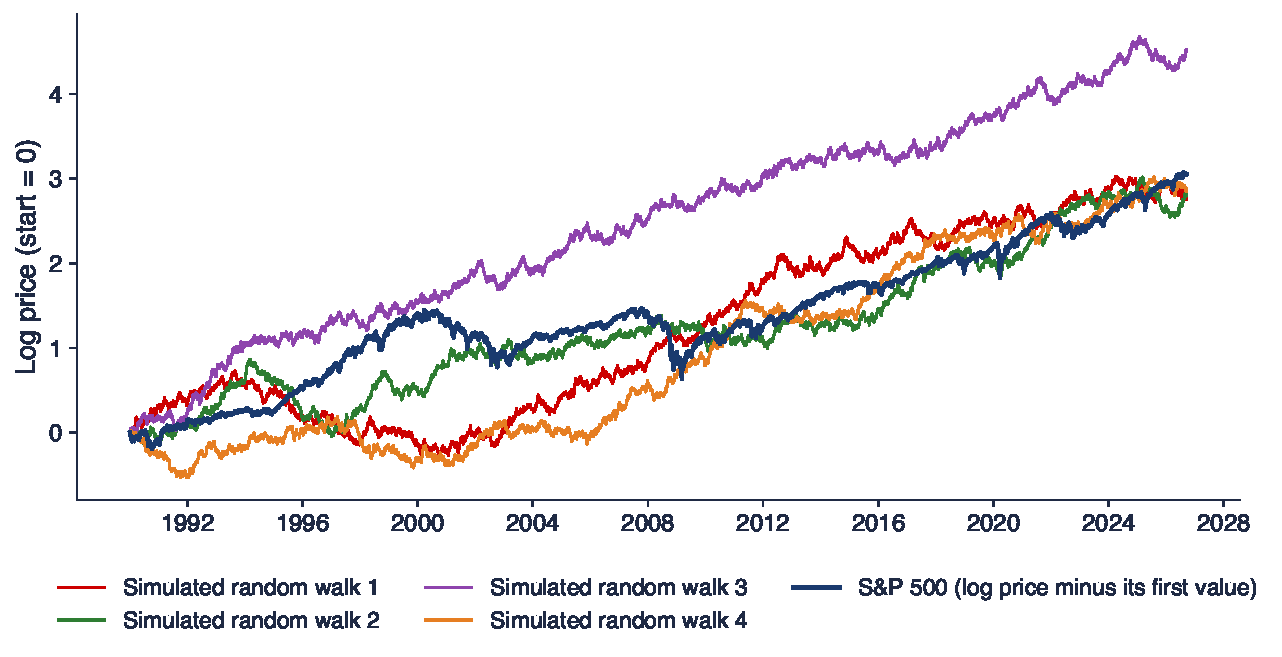
\includegraphics[width=0.97\textwidth,height=0.56\textheight,keepaspectratio]{sfm_ch7_rw_paths.pdf}
\end{center}
\vspace{-0.25cm}
\begin{itemize}
    \item Four random walks with i.i.d.\ Normal steps (mean $0.033\%$, standard deviation $1.13\%$ per day, as the S\&P 500) and the S\&P 500 log price since 1990
    \item \textbf{Question for the room}: without the legend, could you tell which path is real?
    \item \textbf{Answer}: hardly; booms and long falls appear in pure noise too (end values: $2.76$ to $4.50$; S\&P 500: $3.06$)
\end{itemize}
\sfmquantlet{Ch_07}{SFM_ch7_random_walk}
\end{frame}

\begin{frame}{1965: Properly Anticipated Prices Fluctuate Randomly}
\itemsize{\small}
\begin{columns}[T]
\begin{column}{0.54\textwidth}
\begin{itemize}
    \item Paul Samuelson \refSamuelson: if prices already contain all that traders expect, the next change is unpredictable
    \begin{itemize}
        \item formally: the price is a \textbf{martingale}, $E[P_{t+1} \mid \mathcal{F}_t] = P_t$ (\sfmchlink{https://danpele.github.io/SFM/EN/Courses/chapter4_probability.pdf}{Chapter 4})
        \item $\mathcal{F}_t$: the information available at time $t$
    \end{itemize}
    \item Randomness of price changes is a sign of a market that works, not of chaos
    \item \refFamaC: daily returns of the 30 Dow Jones stocks show almost no autocorrelation
\end{itemize}
\end{column}
\begin{column}{0.42\textwidth}
\centering
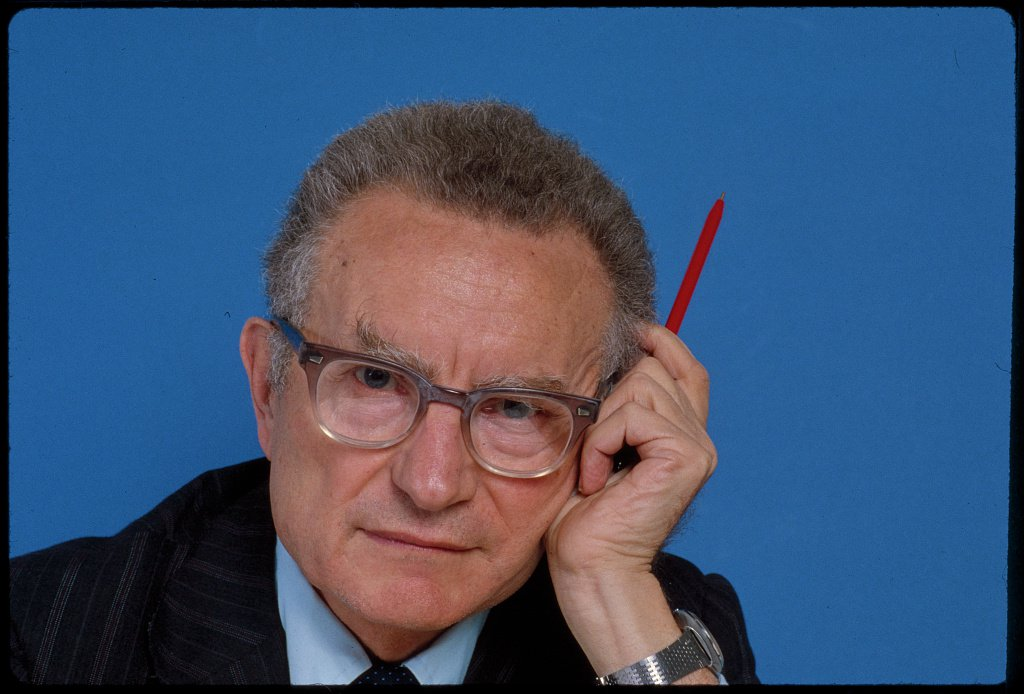
\includegraphics[height=0.34\textheight]{ch7_samuelson.jpg}\\[1mm]
\imgcap{Paul A. Samuelson (1915--2009), Nobel Prize 1970}
\imgcredit{https://commons.wikimedia.org/wiki/File:Paul_A._Samuelson,_economist.jpg}{Photo: Bernard Gotfryd (1970--1975); public domain; Wikimedia Commons}
\end{column}
\end{columns}
\end{frame}

\begin{frame}{Does Yesterday Predict Today?}
\itemsize{\footnotesize}
\begin{center}
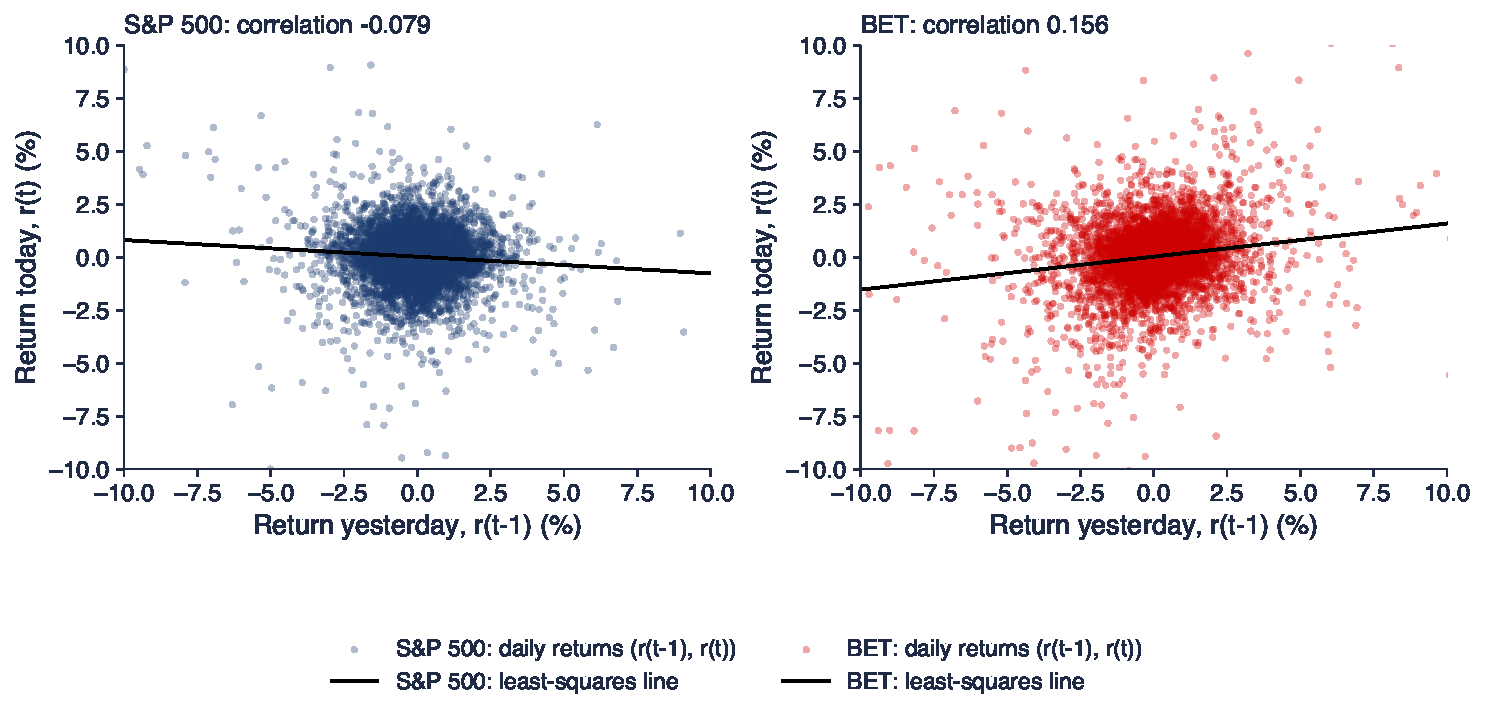
\includegraphics[width=0.97\textwidth,height=0.58\textheight,keepaspectratio]{sfm_ch7_scatter_lag.pdf}
\end{center}
\vspace{-0.25cm}
\begin{itemize}
    \item Each point: (return yesterday, return today); the line: least squares; its slope is the first autocorrelation $\hat\rho(1)$
    \item S\&P 500: $\hat\rho(1) = -0.079$ (a slight reversal); BET: $\hat\rho(1) = 0.156$ (a slight continuation); are these numbers different from zero?
\end{itemize}
\sfmquantlet{Ch_07}{SFM_ch7_random_walk}
\end{frame}

\begin{frame}{Recap: Can Prices Be Predicted?}
\itemsize{\small}
\begin{itemize}
    \item From Bachelier (1900) to Samuelson (1965): price changes look random, and economics explains why
    \item Professional investors rarely beat the market after costs
    \item Daily autocorrelations are small but not zero: we need tests, not impressions
\end{itemize}
\end{frame}


%=============================================================================
\section{Efficient Markets}
%=============================================================================

\begin{frame}{What Is an Efficient Market?}
\itemsize{\small}
\begin{columns}[T]
\begin{column}{0.60\textwidth}
\begin{itemize}
    \item \textbf{EMH} (efficient market hypothesis) \refFamaA: prices ``fully reflect'' the available information $\Omega_t$
    \begin{itemize}
        \item no trading rule based on $\Omega_t$ earns more than the return that compensates its risk
        \item prices move only on \textbf{news}: information that was not in $\Omega_t$
    \end{itemize}
    \item Efficiency is relative to an information set
    \begin{itemize}
        \item the smaller $\Omega_t$, the weaker the claim and the easier the test
    \end{itemize}
    \item Efficient does not mean ``returns are zero'': the expected return pays for risk
\end{itemize}
\end{column}
\begin{column}{0.36\textwidth}
\centering
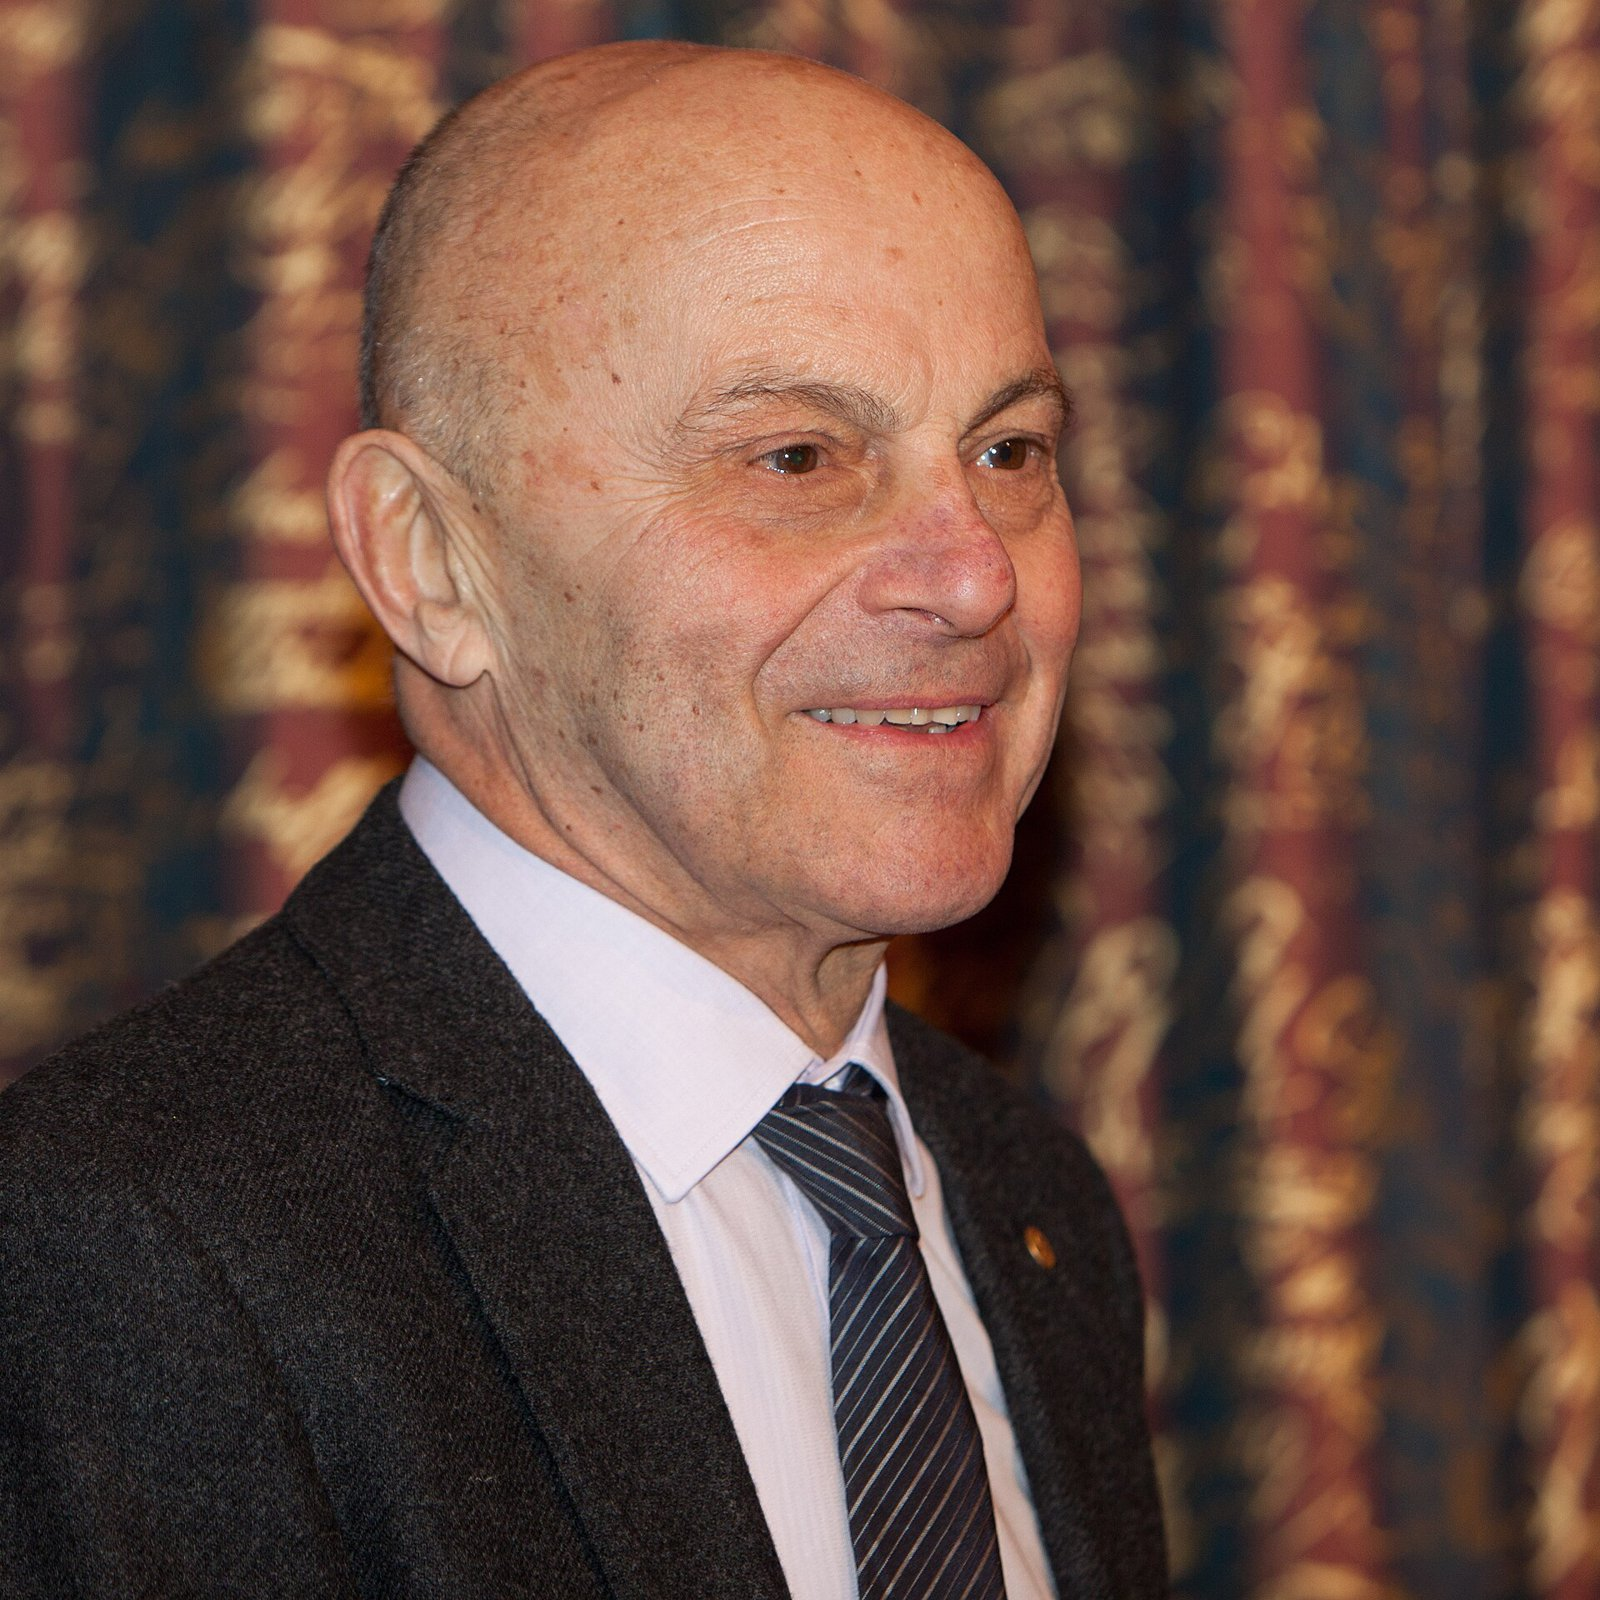
\includegraphics[height=0.42\textheight]{ch0_fama_2013.jpg}\\[1mm]
\imgcap{Eugene F. Fama, Nobel Prize 2013}
\imgcredit{https://commons.wikimedia.org/wiki/File:Eugene_Fama_at_Nobel_Prize,_2013.jpg}{Photo: Bengt Nyman (2013); CC BY 2.0; Wikimedia Commons}
\end{column}
\end{columns}
\end{frame}

\begin{frame}{Three Forms of Efficiency}
\itemsize{\small}
\begin{center}
\footnotesize
\begin{tabular}{>{\raggedright\arraybackslash}p{1.8cm}>{\raggedright\arraybackslash}p{3.2cm}>{\raggedright\arraybackslash}p{3.0cm}>{\raggedright\arraybackslash}p{2.9cm}}
\toprule
\textbf{Form} & \textbf{Information set $\Omega_t$} & \textbf{What cannot earn excess returns} & \textbf{Typical test} \\
\midrule
Weak & past prices and returns & technical analysis, chart patterns & autocorrelation, runs, variance ratio \\
Semi-strong & all public information & fundamental analysis of public data & event studies \\
Strong & all information, also private & insider information & returns of insiders and fund managers \\
\bottomrule
\end{tabular}
\end{center}
\begin{itemize}
    \item The forms are nested: strong $\Rightarrow$ semi-strong $\Rightarrow$ weak; a rejection of the weak form rejects all three
    \item This chapter tests mainly the weak form: past prices are free data for everyone \refFamaA, \refFamaB
\end{itemize}
\end{frame}

\begin{frame}{The Fair-Game Model}
\itemsize{\small}
\begin{itemize}
    \item Let $r_{t+1}$ be the return of an asset and $E[r_{t+1} \mid \Omega_t]$ its \textbf{equilibrium expected return} (the return that pays for its risk)
    \begin{itemize}
        \item the \textbf{excess return} (surprise): $z_{t+1} = r_{t+1} - E[r_{t+1} \mid \Omega_t]$
    \end{itemize}
    \item \textbf{Fair game}: $E[z_{t+1} \mid \Omega_t] = 0$
    \begin{itemize}
        \item forecast errors are zero on average whatever we know at time $t$
        \item a rule that invests $w(\Omega_t)$ earns $E[w(\Omega_t)\, z_{t+1}] = 0$ in excess of equilibrium
    \end{itemize}
    \item With a constant expected return $\mu$: $E[r_{t+1} \mid \Omega_t] = \mu$; returns minus $\mu$ are a \textbf{martingale difference}
    \item Nothing here says the variance is constant or the distribution is Normal
\end{itemize}
\end{frame}

\begin{frame}{The Joint-Hypothesis Problem}
\itemsize{\small}
\begin{itemize}
    \item To test efficiency we must know the equilibrium expected return $E[r_{t+1} \mid \Omega_t]$
    \begin{itemize}
        \item this needs a model of equilibrium: constant mean, CAPM (capital asset pricing model), factor models
    \end{itemize}
    \item Every test of efficiency is a \textbf{joint test} of efficiency and of the model \refFamaB
    \begin{itemize}
        \item a rejection may mean an inefficient market, or a wrong model of expected returns
        \item efficiency alone can never be rejected
    \end{itemize}
    \item For daily returns the problem is small: daily expected returns are tiny (about $0.033\%$ for the S\&P 500), so any reasonable model gives almost the same answer
\end{itemize}
\end{frame}

\begin{frame}{The Grossman--Stiglitz Paradox}
\itemsize{\small}
\begin{itemize}
    \item Information is costly to collect and to analyse \refGS
    \begin{itemize}
        \item if prices reflected all information perfectly, nobody would be paid for collecting it
        \item then nobody would collect it, and prices could not reflect it
    \end{itemize}
    \item Conclusion: a market can only be \textbf{nearly} efficient
    \begin{itemize}
        \item small inefficiencies pay informed traders for their costs
        \item the question becomes ``how efficient, where and when?'', not ``yes or no?''
    \end{itemize}
    \item This view leads to the adaptive markets hypothesis of Section 8
\end{itemize}
\end{frame}

\begin{frame}{2013: One Nobel Prize, Two Views}
\itemsize{\footnotesize}
\begin{columns}[T]
\begin{column}{0.48\textwidth}
\centering
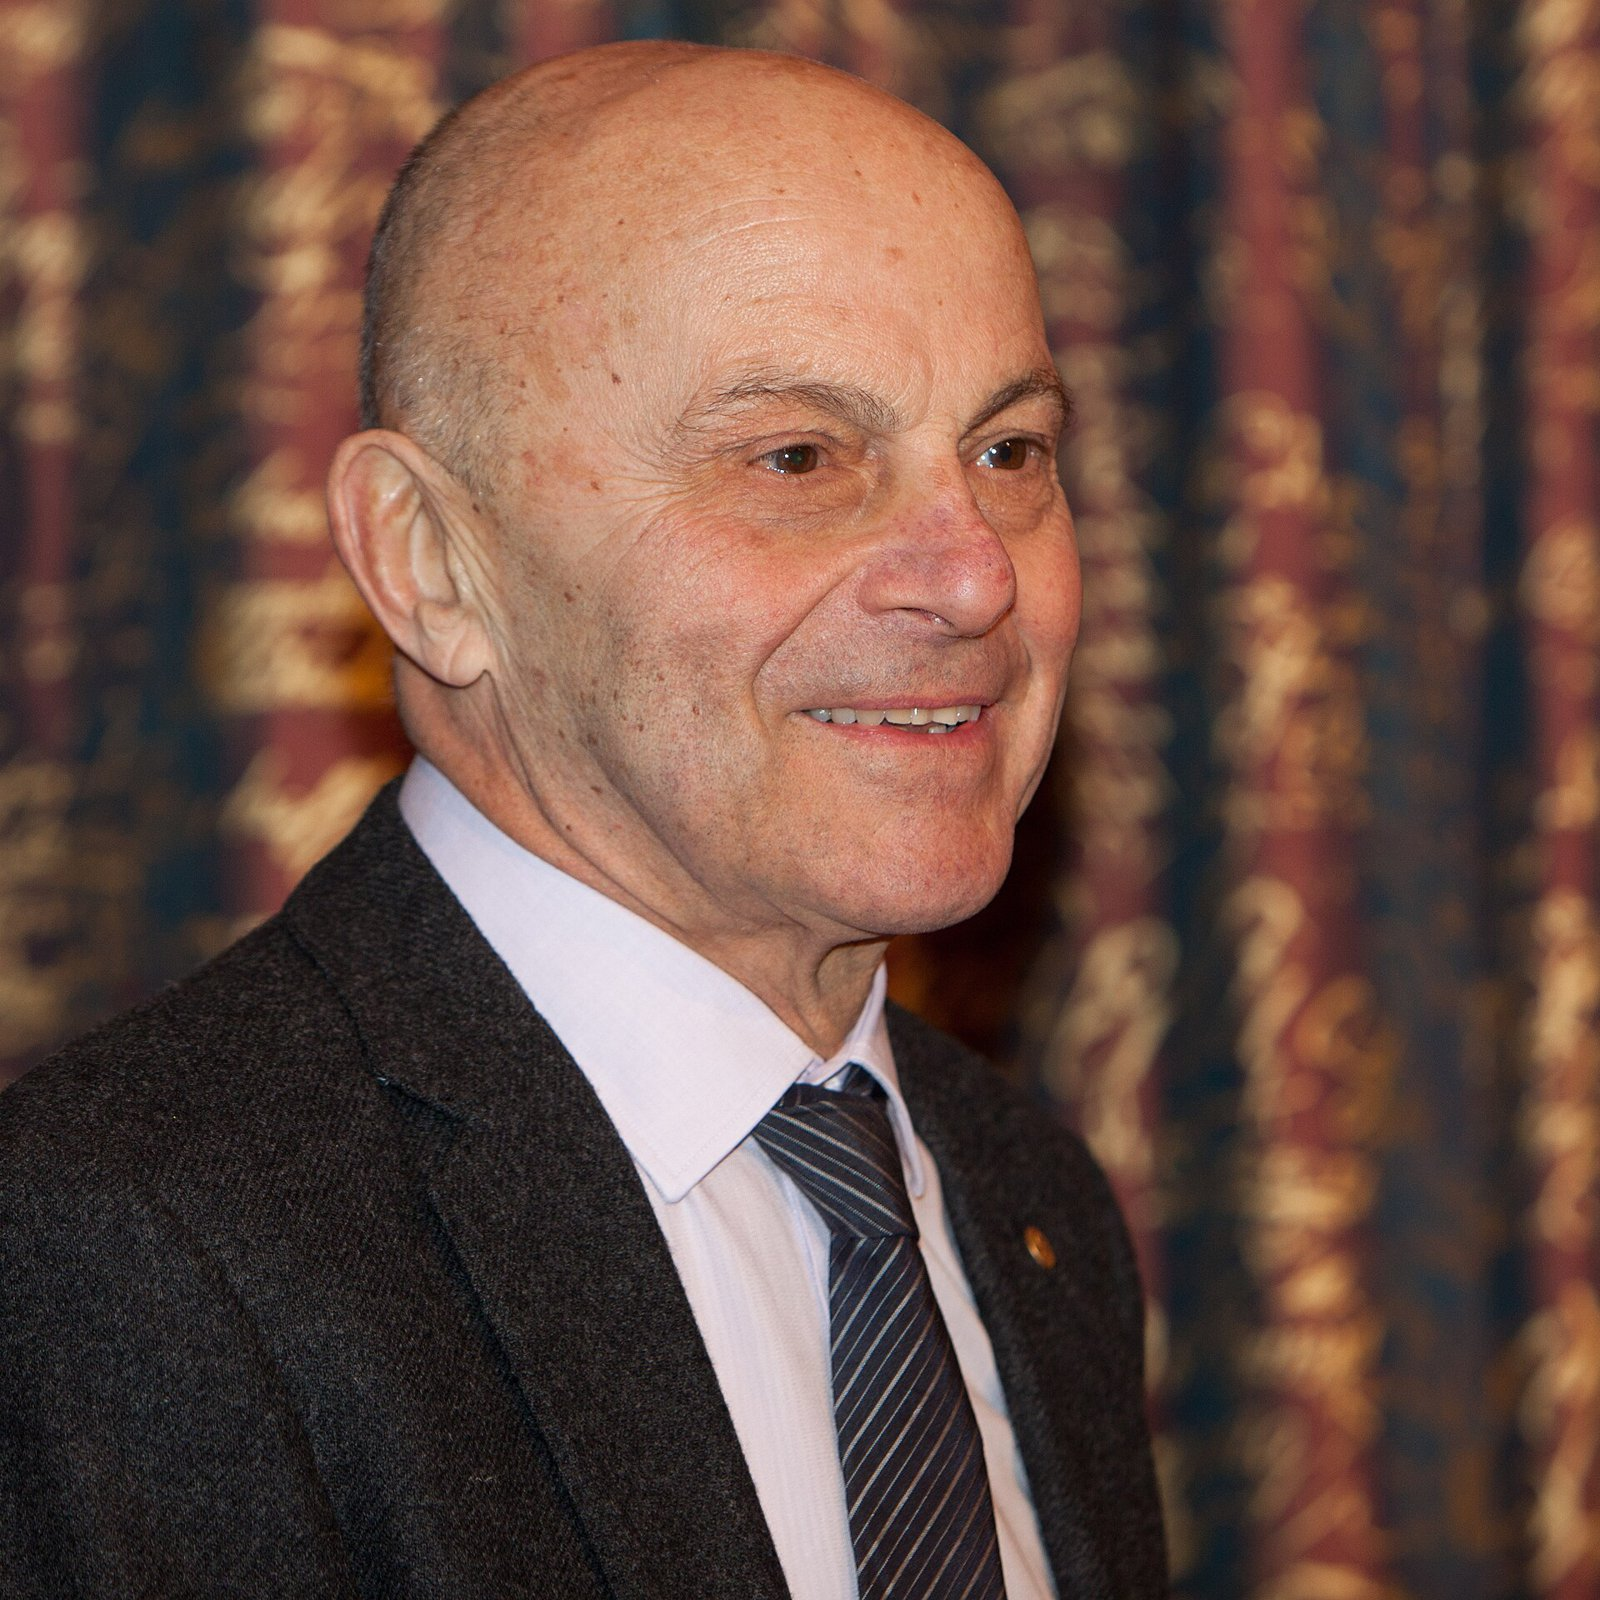
\includegraphics[height=0.38\textheight]{ch0_fama_2013.jpg}\\[1mm]
\imgcap{Eugene F. Fama: prices are hard to predict over days and weeks}
\imgcredit{https://commons.wikimedia.org/wiki/File:Eugene_Fama_at_Nobel_Prize,_2013.jpg}{Photo: Bengt Nyman (2013); CC BY 2.0; Wikimedia Commons}
\end{column}
\begin{column}{0.48\textwidth}
\centering
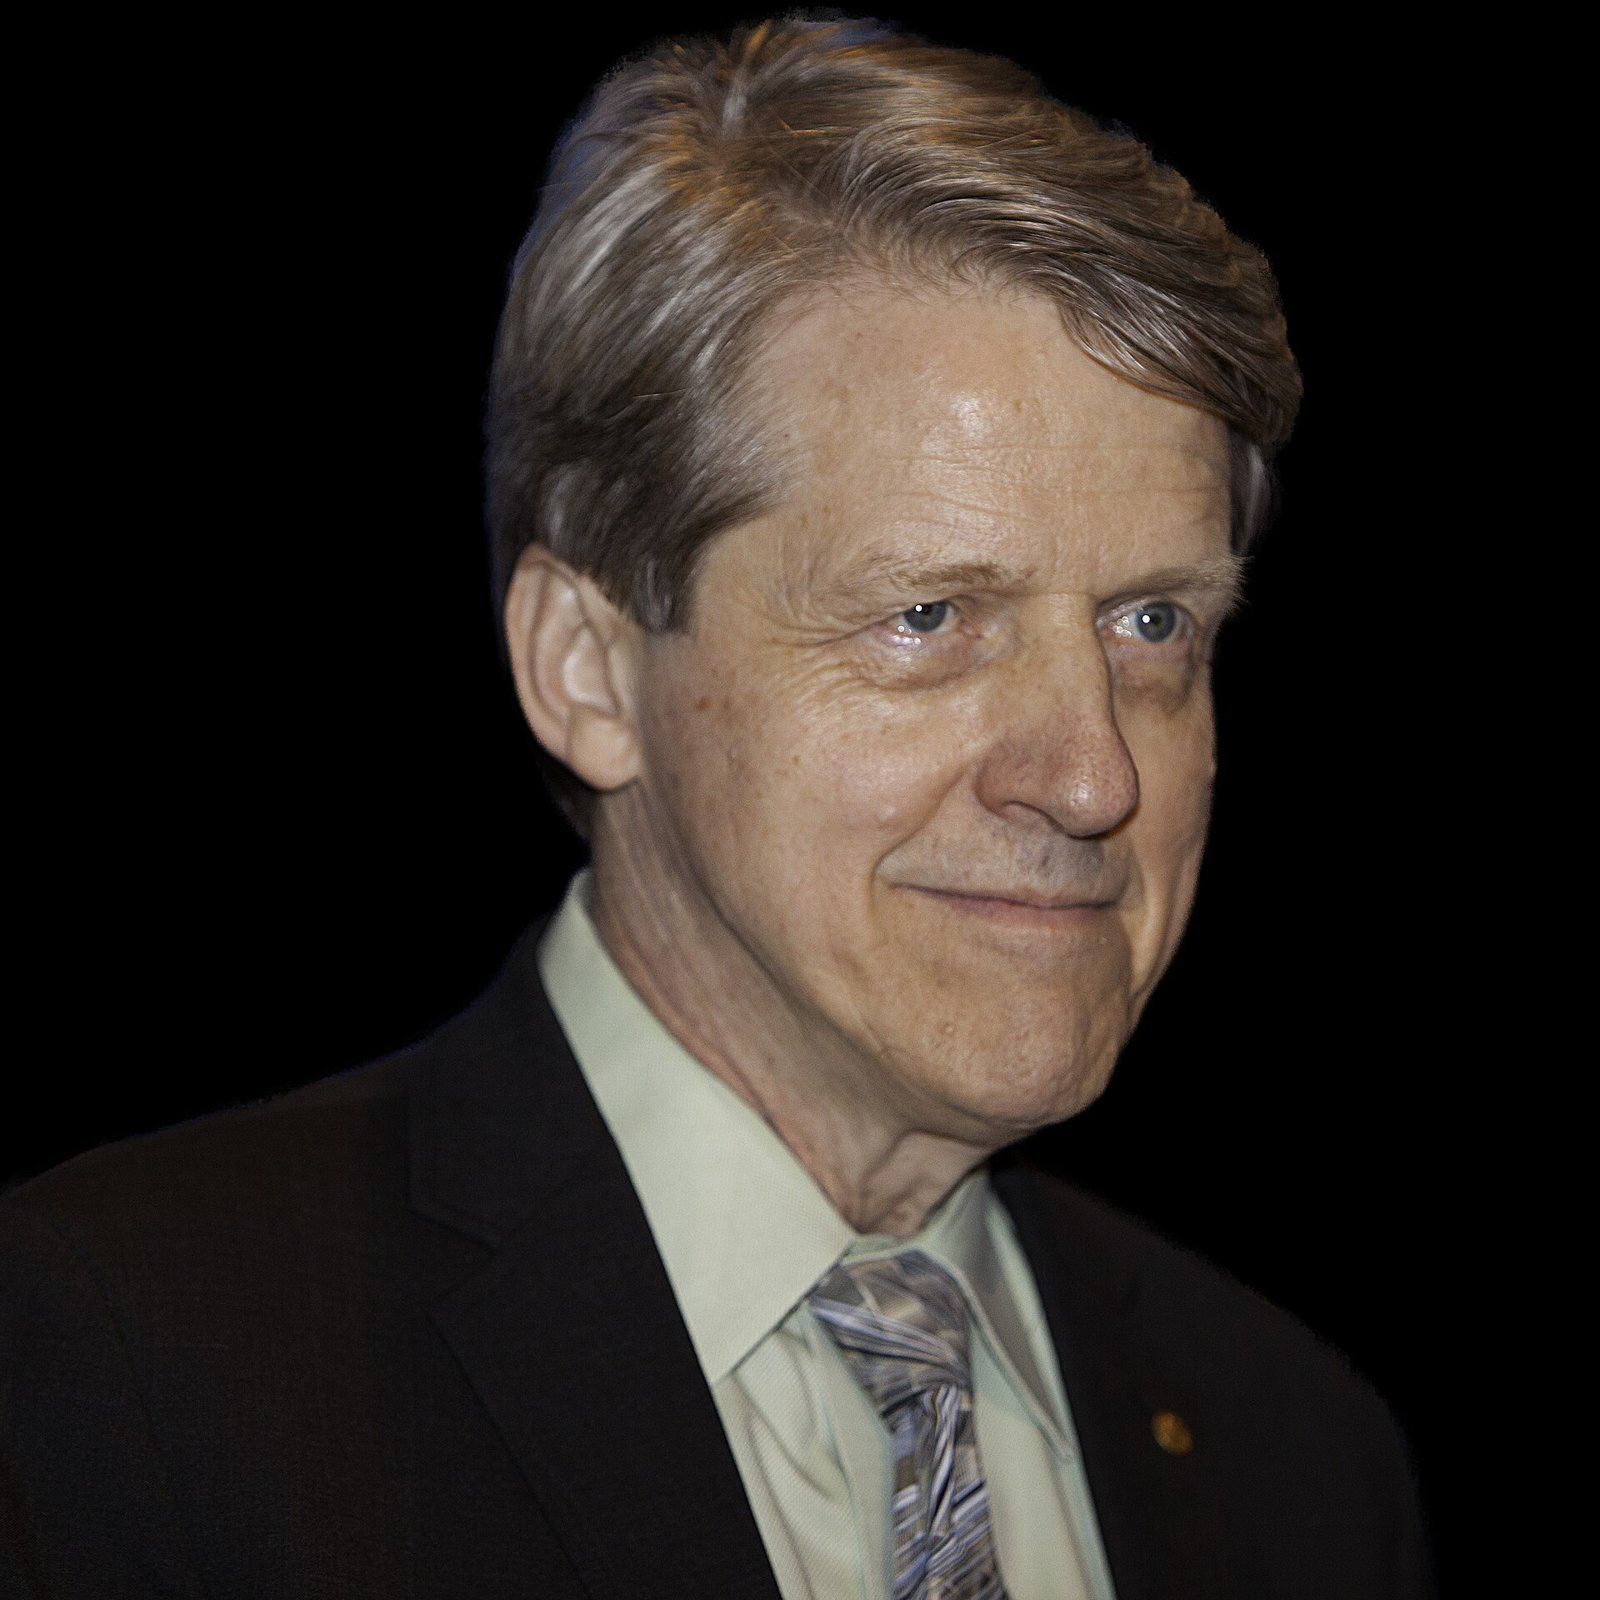
\includegraphics[height=0.38\textheight]{ch7_shiller_2013.jpg}\\[1mm]
\imgcap{Robert J. Shiller: prices swing too much compared with fundamentals}
\imgcredit{https://commons.wikimedia.org/wiki/File:Robert_J._Shiller_(50372668186).jpg}{Photo: Bengt Nyman (2013); CC BY 2.0; Wikimedia Commons}
\end{column}
\end{columns}\begin{itemize}
    \item Both are right, at different horizons: short-run returns are almost unpredictable; long-run returns are partly predictable from valuation ratios
\end{itemize}
\end{frame}

\begin{frame}{Recap: Efficient Markets}
\itemsize{\small}
\begin{itemize}
    \item Efficiency is defined relative to an information set: weak, semi-strong, strong
    \item Fair game: excess returns are unpredictable given $\Omega_t$
    \item Every test is a joint test with a model of expected returns
    \item Costly information makes perfect efficiency impossible \refGS
\end{itemize}
\end{frame}


%=============================================================================
\section{Random Walk Hypotheses}
%=============================================================================

\begin{frame}{The Random Walk Model of Log Prices}
\itemsize{\small}
\begin{itemize}
    \item Log price $p_t = \ln P_t$; \textbf{random walk with drift} $\mu$: $p_t = \mu + p_{t-1} + \varepsilon_t$
    \begin{itemize}
        \item the return $r_t = p_t - p_{t-1} = \mu + \varepsilon_t$: the increments $\varepsilon_t$ have mean 0
        \item by recursion: $p_t = p_0 + \mu t + \sum_{s=1}^{t} \varepsilon_s$: every shock is \textbf{permanent}
    \end{itemize}
    \item If the $\varepsilon_t$ are uncorrelated with variance $\sigma^2$:
    \begin{itemize}
        \item $E[p_t] = p_0 + \mu t$ and $\mathrm{Var}(p_t - p_0) = t\sigma^2$: the uncertainty grows with the horizon
        \item the $q$-day return $r_t(q) = r_t + \dots + r_{t-q+1}$ has $\mathrm{Var}(r_t(q)) = q\sigma^2$
    \end{itemize}
    \item Log prices, not prices: $P_t$ cannot become negative, and log returns add over time (\sfmchlink{https://danpele.github.io/SFM/EN/Courses/chapter1_data_returns_indicators.pdf}{Chapter 1})
\end{itemize}
\end{frame}

\begin{frame}{Three Random Walk Hypotheses}
\itemsize{\small}
\begin{itemize}
    \item \textbf{RW1} (i.i.d.\ increments): $\varepsilon_t$ independent and identically distributed, $\varepsilon_t \sim \mathrm{IID}(0, \sigma^2)$ \refCLM
    \begin{itemize}
        \item the strongest: no function of the past predicts any function of the future
    \end{itemize}
    \item \textbf{RW2} (independent increments): $\varepsilon_t$ independent, but not identically distributed
    \begin{itemize}
        \item allows the variance to change over time in a way that is not predictable from the past (regimes)
    \end{itemize}
    \item \textbf{RW3} (uncorrelated increments): $\mathrm{Cov}(\varepsilon_t, \varepsilon_{t-k}) = 0$ for all $k \ne 0$
    \begin{itemize}
        \item the weakest: allows $\mathrm{Cov}(\varepsilon_t^2, \varepsilon_{t-k}^2) \ne 0$, that is, volatility clustering
    \end{itemize}
    \item Nested: RW1 $\Rightarrow$ RW2 $\Rightarrow$ RW3; tests of RW3 use only autocorrelations of returns
\end{itemize}
\end{frame}

\begin{frame}{What Each Hypothesis Allows}
\itemsize{\small}
\begin{center}
\footnotesize
\begin{tabular}{lcccc}
\toprule
\textbf{Property of the returns} & RW1 & RW2 & RW3 & \textbf{Martingale} \\
\midrule
$\mathrm{Corr}(r_t, r_{t-k}) = 0$ & yes & yes & yes & yes \\
$E[r_t \mid \text{past}] = \mu$ (unpredictable mean) & yes & yes & not always & yes \\
constant variance & yes & no & no & no \\
volatility clustering allowed & no & no & yes & yes \\
GARCH returns (\sfmchlink{https://danpele.github.io/SFM/EN/Courses/chapter9_arch_garch_models.pdf}{Chapter 9}) satisfy it & no & no & yes & yes \\
\bottomrule
\end{tabular}
\end{center}
\begin{itemize}
    \item \textbf{GARCH} (generalised autoregressive conditional heteroskedasticity): the variance of tomorrow depends on today's shocks; the mean stays unpredictable
    \item Weak-form efficiency needs only a martingale (or RW3), not RW1
\end{itemize}
\end{frame}

\begin{frame}{Martingale and Random Walk}
\itemsize{\small}
\begin{itemize}
    \item $\{p_t - \mu t\}$ is a \textbf{martingale} if $E[p_{t+1} - \mu(t+1) \mid \mathcal{F}_t] = p_t - \mu t$ \refSamuelson
    \begin{itemize}
        \item equivalently, $E[r_{t+1} - \mu \mid \mathcal{F}_t] = 0$: the returns minus $\mu$ are a martingale difference
        \item a martingale difference with finite variance is uncorrelated: martingale $\Rightarrow$ RW3
    \end{itemize}
    \item RW1 and RW2 imply the martingale; the converse fails: a martingale may have predictable variance
    \item \textbf{Question for the room}: does volatility clustering contradict weak-form efficiency?
    \begin{itemize}
        \item \textbf{Answer}: no; it rejects RW1 and RW2, but a predictable variance gives no predictable return; the martingale and RW3 survive
    \end{itemize}
\end{itemize}
\end{frame}

\begin{frame}{Worked Example: How Risk Grows with the Horizon}
\itemsize{\small}
\begin{itemize}
    \item S\&P 500 since 1990: daily standard deviation $\hat\sigma = 1.13\%$
    \begin{itemize}
        \item under a random walk, $\mathrm{sd}(r_t(q)) = \sigma\sqrt{q}$
    \end{itemize}
    \item Step by step
    \begin{itemize}
        \item one week, $q = 5$: $1.13 \times \sqrt{5} = 1.13 \times 2.24 = 2.53\%$
        \item one month, $q = 20$: $1.13 \times 4.47 = 5.07\%$
        \item one year, $q = 250$: $1.13 \times 15.81 = 17.92\%$
    \end{itemize}
    \item This is the ``square-root-of-time rule'' used to scale VaR and volatility
    \item If returns are autocorrelated, the rule fails: the variance-ratio test of Section 7 measures by how much
\end{itemize}
\end{frame}

\begin{frame}{Recap: Random Walk Hypotheses}
\itemsize{\small}
\begin{itemize}
    \item $p_t = \mu + p_{t-1} + \varepsilon_t$: permanent shocks, $\mathrm{Var}(r_t(q)) = q\sigma^2$
    \item RW1 (i.i.d.) $\Rightarrow$ RW2 (independent) $\Rightarrow$ RW3 (uncorrelated)
    \item Martingale: unpredictable mean, possibly predictable variance; the right null for efficiency
\end{itemize}
\end{frame}


%=============================================================================
\section{White Noise and the Autocorrelation Function}
%=============================================================================

\begin{frame}{White Noise and Autocorrelation}
\itemsize{\small}
\begin{itemize}
    \item \textbf{Autocovariance} at lag $k$: $\gamma(k) = \mathrm{Cov}(x_t, x_{t-k})$; \textbf{autocorrelation}: $\rho(k) = \gamma(k)/\gamma(0)$
    \begin{itemize}
        \item the \textbf{ACF} (autocorrelation function): $k \mapsto \rho(k)$, $k = 1, 2, \dots$
    \end{itemize}
    \item \textbf{White noise}: mean 0, constant variance $\sigma^2$, $\rho(k) = 0$ for every $k \ne 0$
    \begin{itemize}
        \item i.i.d.\ noise is white noise; Gaussian white noise is i.i.d.\ $N(0, \sigma^2)$
        \item white noise need not be independent: GARCH returns are white noise but not i.i.d.
    \end{itemize}
    \item \textbf{Sample ACF}: $\hat\rho(k) = \sum_{t=k+1}^{T}(x_t - \bar x)(x_{t-k} - \bar x)\big/\sum_{t=1}^{T}(x_t - \bar x)^2$
    \begin{itemize}
        \item for i.i.d.\ data, $\hat\rho(k) \approx N(0, 1/T)$: 95\% band $\pm 1.96/\sqrt{T}$
    \end{itemize}
\end{itemize}
\end{frame}

\begin{frame}{Gaussian White Noise and Its Sample ACF}
\itemsize{\footnotesize}
\begin{center}
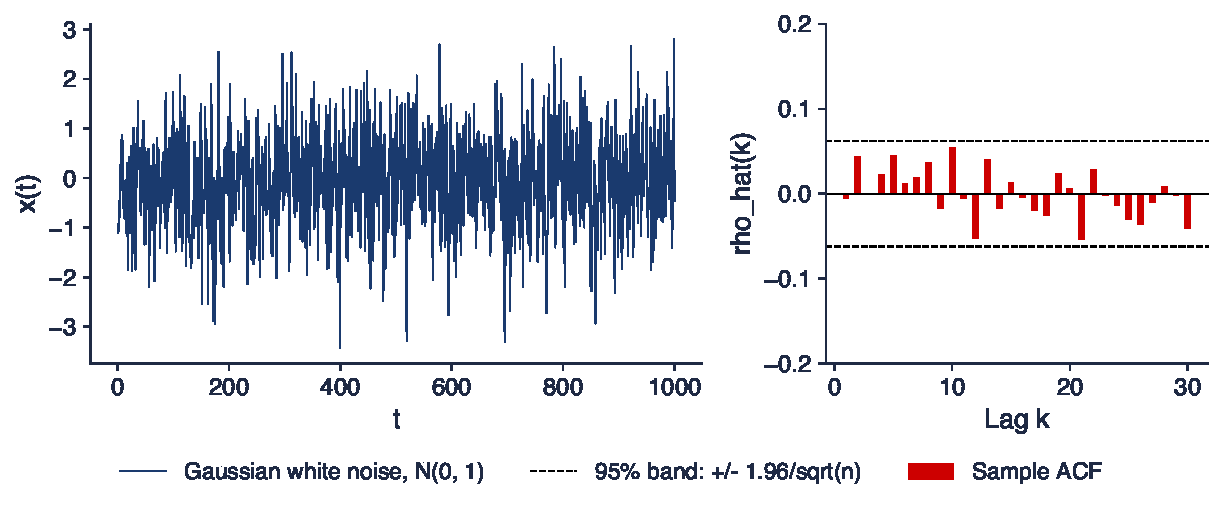
\includegraphics[width=0.97\textwidth,height=0.56\textheight,keepaspectratio]{sfm_ch7_white_noise.pdf}
\end{center}
\vspace{-0.25cm}
\begin{itemize}
    \item Left: 1\,000 draws from $N(0, 1)$ (as in SFEtimewn); right: $\hat\rho(1), \dots, \hat\rho(30)$ with the band $\pm 1.96/\sqrt{1000} = \pm 0.062$
    \item Here 0 of 30 autocorrelations fall outside the band; with 30 lags we expect about 1.5 by chance alone
\end{itemize}
\sfmquantlet{Ch_07}{SFM_ch7_white_noise_acf}
\end{frame}

\begin{frame}{The ACF of AR and MA Processes}
\itemsize{\small}
\begin{itemize}
    \item \textbf{AR(1)} (autoregressive): $x_t = \alpha x_{t-1} + \varepsilon_t$, $|\alpha| < 1$: $\rho(k) = \alpha^k$
    \begin{itemize}
        \item geometric decay; alternating signs if $\alpha < 0$; example: $\alpha = 0.9 \Rightarrow \rho(3) = 0.9^3 = 0.729$
    \end{itemize}
    \item \textbf{AR(2)}: $x_t = \alpha_1 x_{t-1} + \alpha_2 x_{t-2} + \varepsilon_t$: $\rho(1) = \alpha_1/(1 - \alpha_2)$, $\rho(k) = \alpha_1\rho(k-1) + \alpha_2\rho(k-2)$
    \begin{itemize}
        \item $\alpha_1 = 0.5$, $\alpha_2 = 0.4$: $\rho(1) = 0.5/0.6 = 0.833$, $\rho(2) = 0.5 \times 0.833 + 0.4 = 0.817$
    \end{itemize}
    \item \textbf{MA(1)} (moving average): $x_t = \varepsilon_t + \beta\varepsilon_{t-1}$: $\rho(1) = \beta/(1 + \beta^2)$, $\rho(k) = 0$ for $k \ge 2$
    \begin{itemize}
        \item $\beta = 0.5$: $\rho(1) = 0.5/1.25 = 0.40$; an MA($q$) has an ACF that cuts off after lag $q$
    \end{itemize}
    \item The shape of the ACF tells the type of dependence: slow decay (AR), cut-off (MA), nothing (white noise)
\end{itemize}
\end{frame}

\begin{frame}{Theoretical and Sample ACF of Six Processes}
\itemsize{\footnotesize}
\begin{center}
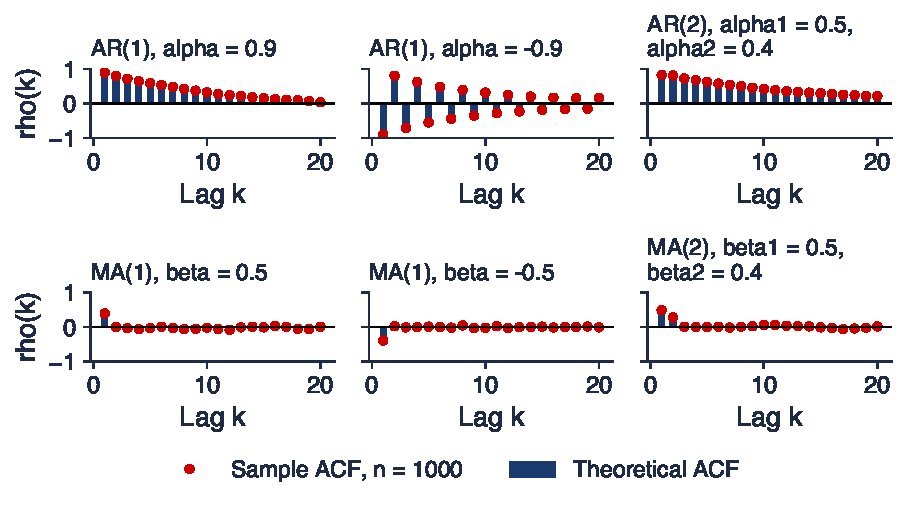
\includegraphics[width=0.97\textwidth,height=0.60\textheight,keepaspectratio]{sfm_ch7_acf_processes.pdf}
\end{center}
\vspace{-0.25cm}
\begin{itemize}
    \item Bars: theoretical $\rho(k)$; points: sample ACF of one simulated path of 1\,000 values (SFEacfar1, SFEacfar2, SFEacfma1, SFEacfma2)
    \item A random walk is the limit $\alpha \to 1$ of the AR(1): its ACF would not decay at all
\end{itemize}
\sfmquantlet{Ch_07}{SFM_ch7_white_noise_acf}
\end{frame}

\begin{frame}{The ACF of Daily Returns}
\itemsize{\footnotesize}
\begin{center}
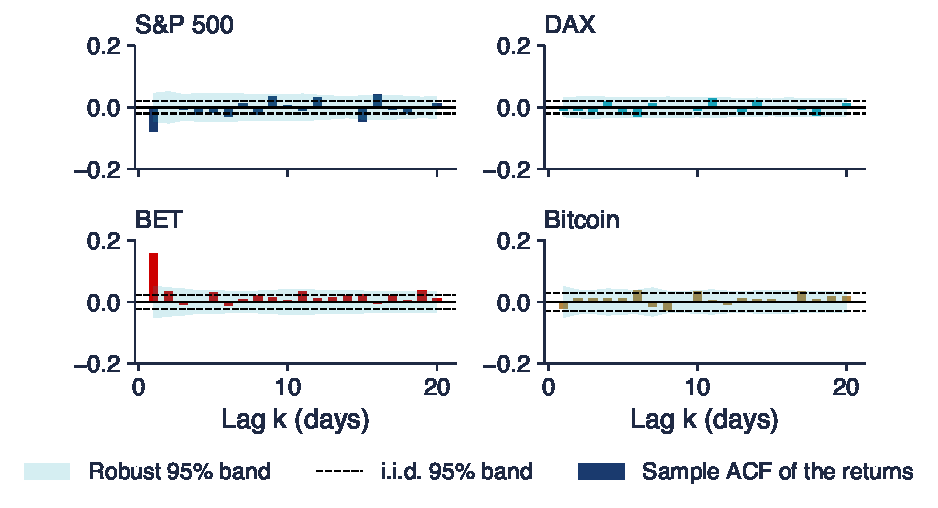
\includegraphics[width=0.97\textwidth,height=0.62\textheight,keepaspectratio]{sfm_ch7_acf_returns.pdf}
\end{center}
\vspace{-0.25cm}
\begin{itemize}
    \item Bars: $\hat\rho(1), \dots, \hat\rho(20)$; dashed: the i.i.d.\ band $\pm 1.96/\sqrt{T}$; shaded: the robust band (next slide)
\end{itemize}
\sfmquantlet{Ch_07}{SFM_ch7_autocorrelation_tests}
\end{frame}

\begin{frame}{Reading the ACF of Returns}
\itemsize{\small}
\begin{itemize}
    \item First autocorrelations: S\&P 500 $-0.079$, DAX $-0.009$, BET $0.156$, Bitcoin $-0.022$
    \begin{itemize}
        \item only the S\&P 500 and the BET stand out at lag 1, with opposite signs
    \end{itemize}
    \item The \textbf{robust} band: $\pm 1.96\sqrt{\hat\delta(k)/T}$, $\hat\delta(k) = T\sum_t e_t^2 e_{t-k}^2/(\sum_t e_t^2)^2$, $e_t = r_t - \bar r$ \refLM
    \begin{itemize}
        \item i.i.d.\ returns: $\hat\delta(k) \approx 1$; volatility clustering: large returns follow large returns, so $\hat\delta(k) > 1$
        \item S\&P 500 at lag 1: $\pm 0.046$ instead of $\pm 0.020$
    \end{itemize}
    \item S\&P 500, lags outside the band out of 20: 9 with the i.i.d.\ band, 3 with the robust band
    \item The i.i.d.\ band tests RW1; the robust band tests RW3, the hypothesis that matters for efficiency
\end{itemize}\sfmquantlet{Ch_07}{SFM_ch7_autocorrelation_tests}
\end{frame}

\begin{frame}{Returns Are Almost Uncorrelated, Their Size Is Not}
\itemsize{\footnotesize}
\begin{center}
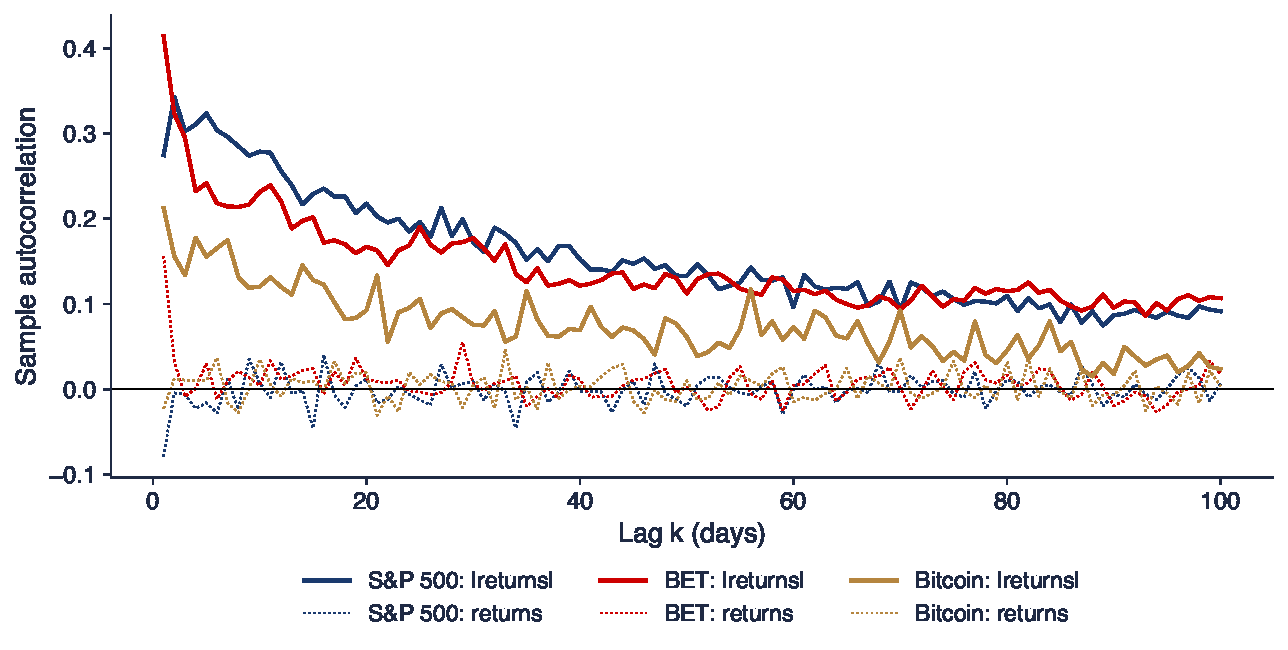
\includegraphics[width=0.97\textwidth,height=0.56\textheight,keepaspectratio]{sfm_ch7_acf_abs.pdf}
\end{center}
\vspace{-0.25cm}
\begin{itemize}
    \item ACF of $|r_t|$: S\&P 500 $0.27$ at lag 1, $0.22$ at lag 20, $0.09$ at lag 100; the returns themselves: dotted lines near 0
    \item Large moves follow large moves: RW1 and RW2 are rejected by eye; RW3 and the martingale are not touched by this chart
\end{itemize}
\sfmquantlet{Ch_07}{SFM_ch7_autocorrelation_tests}
\end{frame}

\begin{frame}{Recap: White Noise and the ACF}
\itemsize{\small}
\begin{itemize}
    \item White noise: uncorrelated; i.i.d.\ noise: independent; GARCH returns: white noise, not i.i.d.
    \item AR: geometric decay of the ACF; MA($q$): cut-off after $q$ lags
    \item Use the robust band $\pm 1.96\sqrt{\hat\delta(k)/T}$ for returns: the i.i.d.\ band is too narrow
\end{itemize}
\end{frame}


%=============================================================================
\section{Testing for Autocorrelation}
%=============================================================================

\begin{frame}{Portmanteau Tests: Box--Pierce and Ljung--Box}
\itemsize{\small}
\begin{itemize}
    \item $H_0$: $\rho(1) = \dots = \rho(m) = 0$; $H_1$: at least one $\rho(k) \ne 0$; one test for $m$ lags together
    \begin{itemize}
        \item ``portmanteau'': a suitcase that carries many autocorrelations at once
    \end{itemize}
    \item Box--Pierce \refBP: $Q_{BP}(m) = T\sum_{k=1}^{m} \hat\rho(k)^2$
    \item \textbf{LB} (Ljung--Box) \refLjung: $Q_{LB}(m) = T(T+2)\sum_{k=1}^{m} \dfrac{\hat\rho(k)^2}{T - k}$, closer to $\chi^2$ in small samples
    \begin{itemize}
        \item under i.i.d.\ returns both $\sim \chi^2(m)$; reject $H_0$ if $Q > \chi^2_{0.95}(m)$; $\chi^2_{0.95}(10) = 18.31$
    \end{itemize}
    \item Choice of $m$: here $m = 10$ (two trading weeks); a larger $m$ dilutes a short-lived effect
\end{itemize}
\end{frame}

\begin{frame}{Worked Example: Ljung--Box Step by Step}
\itemsize{\small}
\begin{itemize}
    \item $T = 1000$ daily returns, $\hat\rho(1) = 0.06$, $\hat\rho(2) = -0.04$, $\hat\rho(3) = 0.03$; test with $m = 3$
    \begin{itemize}
        \item $T\hat\rho(k)^2$: $3.6$, $1.6$, $0.9$; their sum: $Q_{BP}(3) = 6.10$
        \item $Q_{LB}(3) = 1000 \times 1002 \times (0.06^2/999 + 0.04^2/998 + 0.03^2/997) = 6.12$
    \end{itemize}
    \item Decision: $\chi^2_{0.95}(3) = 7.81 > 6.12$: do not reject $H_0$ at 5\%
    \begin{itemize}
        \item note: $\hat\rho(1) = 0.06$ lies just inside the band $\pm 1.96/\sqrt{1000} = \pm 0.062$; the joint test does not reject either
    \end{itemize}
    \item The same numbers with $T = 5000$: $Q$ five times larger, a clear rejection: small autocorrelations become significant in long samples
\end{itemize}
\end{frame}

\begin{frame}{A Portmanteau Test Robust to Volatility Clustering}
\itemsize{\small}
\begin{itemize}
    \item The $\chi^2$ law of $Q_{LB}$ needs $\mathrm{Var}(\hat\rho(k)) = 1/T$: true for i.i.d.\ returns, false with volatility clustering
    \begin{itemize}
        \item then $Q_{LB}$ rejects a true martingale far too often
    \end{itemize}
    \item \textbf{Robust} statistic: divide each $\hat\rho(k)^2$ by its own variance $\hat\delta(k)/T$ \refEL
    \begin{itemize}
        \item $\tilde Q(m) = \sum_{k=1}^{m} \dfrac{T\hat\rho(k)^2}{\hat\delta(k)} \sim \chi^2(m)$ for a martingale difference with finite fourth moment
        \item with i.i.d.\ returns $\hat\delta(k) \approx 1$ and $\tilde Q \approx Q_{BP}$
    \end{itemize}
    \item Rule: test RW1 with $Q_{LB}$; test the martingale (weak-form efficiency) with $\tilde Q$
\end{itemize}
\end{frame}

\begin{frame}{Autocorrelation Tests on Real Data}
\itemsize{\footnotesize}
\begin{center}
\scriptsize
\begin{tabular}{lrrrrrrrrr}
\toprule
& $T$ & $\hat\rho(1)$ & $Q_{LB}(10)$ & p & $\tilde Q(10)$ & p & $Q_{LB}(10)$, $r^2$ & runs $z$ & p \\
\midrule
S\&P 500 & 9\,240 & ${-0.079}$ & $90.8$ & $<$\,0.001 & $18.8$ & 0.043 & $8015$ & ${2.97}$ & 0.003 \\
DAX & 9\,288 & ${-0.009}$ & $21.8$ & 0.016 & $8.6$ & 0.571 & $3747$ & ${1.73}$ & 0.084 \\
BET & 7\,243 & ${0.156}$ & $198.3$ & $<$\,0.001 & $42.9$ & $<$\,0.001 & $2500$ & ${-7.75}$ & $<$\,0.001 \\
Bitcoin & 4\,384 & ${-0.022}$ & $20.2$ & 0.028 & $11.9$ & 0.294 & $213$ & ${2.68}$ & 0.007 \\
TLV & 3\,788 & ${0.010}$ & $29.1$ & 0.001 & $13.2$ & 0.210 & $481$ & ${-1.68}$ & 0.093 \\
SNP & 3\,815 & ${-0.015}$ & $20.7$ & 0.023 & $9.9$ & 0.446 & $505$ & ${1.72}$ & 0.085 \\
BRD & 3\,771 & ${0.032}$ & $19.9$ & 0.030 & $10.8$ & 0.375 & $416$ & ${-3.04}$ & 0.002 \\
TGN & 3\,725 & ${0.055}$ & $28.7$ & 0.001 & $12.3$ & 0.263 & $639$ & ${1.49}$ & 0.136 \\
\bottomrule
\end{tabular}
\end{center}
\begin{itemize}
    \item Classic LB: all eight series reject at 5\%; robust $\tilde Q$: only the S\&P 500 (p = 0.043) and the BET (p = $<$\,0.001)
    \item Squared returns: huge $Q_{LB}$ everywhere: RW1 and RW2 are rejected for every series (volatility clustering)
    \item Start of the series: S\&P 500 and DAX 1990; BET 1997; Bitcoin 2014; BVB stocks 2010 (TLV without 30--31 May 2016, a data error, \sfmchlink{https://danpele.github.io/SFM/EN/Courses/chapter2_classical_distributions_stylised_facts.pdf}{Chapter 2})
\end{itemize}\sfmquantlet{Ch_07}{SFM_ch7_autocorrelation_tests}
\end{frame}

\begin{frame}{The Runs Test}
\itemsize{\small}
\begin{itemize}
    \item A \textbf{run}: a sequence of returns with the same sign; $+ + - + + + - -$ has 4 runs \refWW
    \begin{itemize}
        \item the test uses only the signs: it is \textbf{nonparametric}, insensitive to heavy tails and to volatility
    \end{itemize}
    \item With $n_1$ positive and $n_2$ negative returns, $n = n_1 + n_2$, under independence:
    \begin{itemize}
        \item $E[R] = \dfrac{2n_1n_2}{n} + 1$, \quad $\mathrm{Var}(R) = \dfrac{2n_1n_2(2n_1n_2 - n)}{n^2(n-1)}$, \quad $z = \dfrac{R - E[R]}{\sqrt{\mathrm{Var}(R)}} \approx N(0, 1)$
    \end{itemize}
    \item Too few runs ($z < 0$): signs persist, positive dependence; too many runs ($z > 0$): signs alternate
    \begin{itemize}
        \item BET: 3\,278 runs against 3\,606 expected, $z = -7.75$; S\&P 500: 4\,738 against 4\,596, $z = 2.97$
        \item the same directions as $\hat\rho(1)$: continuation in the BET, reversal in the S\&P 500
    \end{itemize}
\end{itemize}\sfmquantlet{Ch_07}{SFM_ch7_autocorrelation_tests}
\end{frame}

\begin{frame}{Recap: Testing for Autocorrelation}
\itemsize{\small}
\begin{itemize}
    \item $Q_{LB}(m) = T(T+2)\sum \hat\rho(k)^2/(T-k) \sim \chi^2(m)$ under i.i.d.\ returns
    \item With volatility clustering use the robust $\tilde Q$: the verdict changes for six of eight series
    \item Runs test: signs only; too few runs means continuation
    \item $\tilde Q$: reversal in the S\&P 500, continuation in the BET; no rejection for the DAX, Bitcoin and the BVB stocks
\end{itemize}
\end{frame}


%=============================================================================
\section{Unit Roots: Prices against Returns}
%=============================================================================

\begin{frame}{Stationary and Integrated Series}
\itemsize{\small}
\begin{itemize}
    \item \textbf{(Weakly) stationary} series: constant mean, constant variance, $\mathrm{Cov}(x_t, x_{t-k})$ depends only on $k$
    \begin{itemize}
        \item shocks fade away; the series returns to its mean; notation $I(0)$
    \end{itemize}
    \item \textbf{Integrated of order 1}, $I(1)$: not stationary, but its first difference $\Delta x_t = x_t - x_{t-1}$ is
    \begin{itemize}
        \item the random walk is $I(1)$: $p_t$ wanders, $\Delta p_t = r_t$ is stationary
    \end{itemize}
    \item \textbf{Unit root}: in $p_t = \phi\,p_{t-1} + \varepsilon_t$ the case $\phi = 1$; $|\phi| < 1$ gives a stationary AR(1)
    \begin{itemize}
        \item the name: the root of $1 - \phi z = 0$ is $z = 1/\phi = 1$
    \end{itemize}
    \item Question of this section: are log prices $I(1)$ and returns $I(0)$?
\end{itemize}
\end{frame}

\begin{frame}{Why It Matters: Spurious Regression}
\itemsize{\footnotesize}
\begin{center}
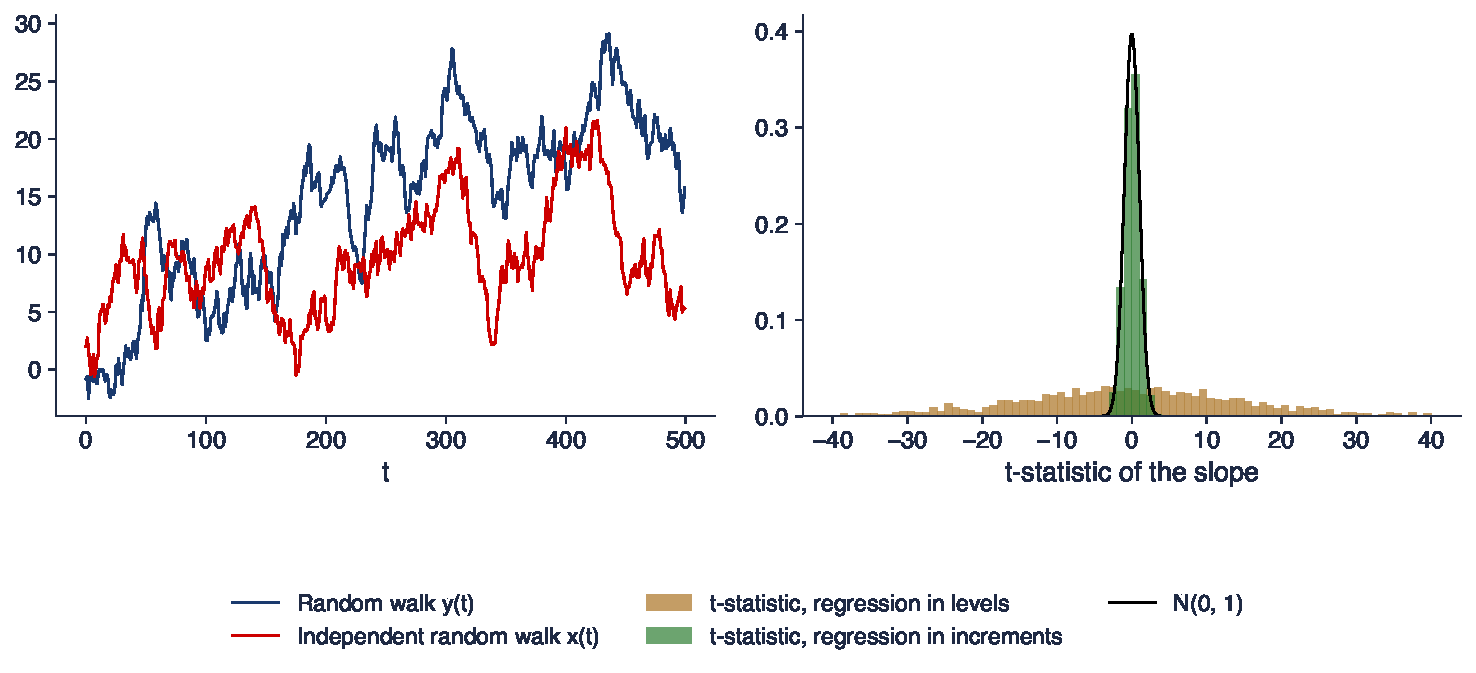
\includegraphics[width=0.97\textwidth,height=0.54\textheight,keepaspectratio]{sfm_ch7_spurious.pdf}
\end{center}
\vspace{-0.25cm}
\begin{itemize}
    \item Regress one random walk on another, independent one ($T = 500$, 2\,000 repetitions) \refGN: $|t| > 1.96$ in 90\% of cases, median $R^2 = 0.17$
    \item On the increments: $|t| > 1.96$ in 5.5\% of cases, as it should be; lesson: test for unit roots before regressing levels ($|t| > 40$ in 2.6\% of cases, not drawn)
\end{itemize}
\sfmquantlet{Ch_07}{SFM_ch7_unit_roots}
\end{frame}

\begin{frame}{The Dickey--Fuller Test}
\itemsize{\small}
\begin{itemize}
    \item Subtract $p_{t-1}$: $\Delta p_t = c + \gamma\, p_{t-1} + \varepsilon_t$ with $\gamma = \phi - 1$ \refDF
    \begin{itemize}
        \item $H_0$: $\gamma = 0$ (unit root); $H_1$: $\gamma < 0$ (stationary); a one-sided test
        \item statistic: $\tau = \hat\gamma/\mathrm{SE}(\hat\gamma)$, the usual $t$-ratio of OLS (ordinary least squares)
    \end{itemize}
    \item Under $H_0$, $\tau$ does \textbf{not} follow a $t$ or Normal law: its critical values are more negative
    \begin{itemize}
        \item 5\% critical values \refMacKinnon: $-2.86$ with a constant, $-3.41$ with a constant and a trend (Normal: $-1.645$)
    \end{itemize}
    \item Three specifications: no constant; constant $c$; constant and trend $c + bt$
    \begin{itemize}
        \item log prices drift upwards: use constant and trend; returns: constant only
    \end{itemize}
\end{itemize}
\end{frame}

\begin{frame}{The Augmented Test and a Worked Example}
\itemsize{\small}
\begin{itemize}
    \item \textbf{ADF} (augmented Dickey--Fuller) \refSD: add lagged differences to remove autocorrelation from $\varepsilon_t$
    \begin{itemize}
        \item $\Delta p_t = c + bt + \gamma\, p_{t-1} + \sum_{j=1}^{L} \delta_j \Delta p_{t-j} + \varepsilon_t$; same $\tau$, same critical values
        \item $L$ chosen by AIC (Akaike information criterion, \sfmchlink{https://danpele.github.io/SFM/EN/Courses/chapter6_model_selection_risk_management.pdf}{Chapter 6}), at most $12(T/100)^{1/4}$
    \end{itemize}
    \item \textbf{Worked example}: BET log price, constant, no lags, $T = 7\,243$
    \begin{itemize}
        \item OLS: $\hat\gamma = -0.00001$, $\mathrm{SE}(\hat\gamma) = 0.00016$
        \item $\tau = -0.00001/0.00016 = -0.09 > -2.86$: do not reject the unit root
        \item a usual $t$-test (critical value $-1.645$) would have rejected it: the wrong distribution gives the wrong answer
    \end{itemize}
\end{itemize}
\end{frame}

\begin{frame}{Phillips--Perron and KPSS}
\itemsize{\small}
\begin{itemize}
    \item \textbf{PP} (Phillips--Perron) \refPP: the Dickey--Fuller regression without lags; $\tau$ is corrected for autocorrelation and heteroskedasticity
    \begin{itemize}
        \item the correction uses a long-run variance with Bartlett weights \refNW; same $H_0$ and critical values as ADF
    \end{itemize}
    \item \textbf{KPSS} (Kwiatkowski--Phillips--Schmidt--Shin) \refKPSS: the hypotheses are \textbf{reversed}
    \begin{itemize}
        \item $H_0$: stationary (around a constant or a trend); $H_1$: unit root
        \item $\mathrm{KPSS} = \sum_{t=1}^{T} S_t^2/(T^2\hat\lambda^2)$, $S_t$ the partial sums of the residuals, $\hat\lambda^2$ their long-run variance
        \item reject stationarity if $\mathrm{KPSS} > 0.463$ (constant) or $> 0.146$ (trend), at 5\%
    \end{itemize}
    \item Use both: ADF/PP ask ``is there evidence against a unit root?''; KPSS asks ``is there evidence against stationarity?''
    \begin{itemize}
        \item ADF does not reject and KPSS rejects: $I(1)$; ADF rejects and KPSS does not: $I(0)$; both or neither reject: inconclusive
    \end{itemize}
\end{itemize}
\end{frame}

\begin{frame}{The BET: Log Price and Returns}
\itemsize{\footnotesize}
\begin{center}
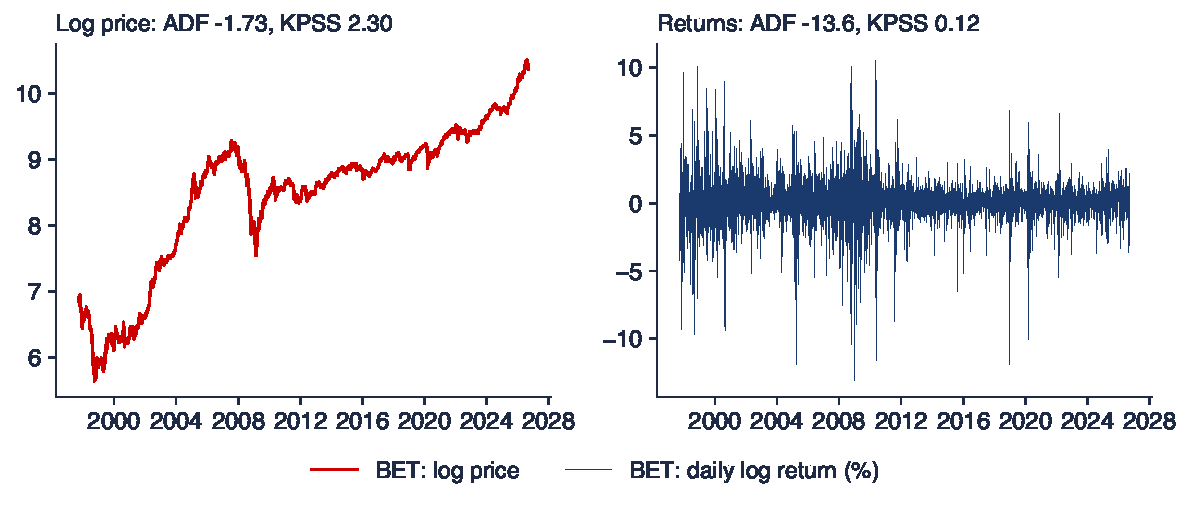
\includegraphics[width=0.97\textwidth,height=0.52\textheight,keepaspectratio]{sfm_ch7_unit_root_bet.pdf}
\end{center}
\vspace{-0.25cm}
\begin{itemize}
    \item Log price: ADF $-1.73$ (p = 0.736), KPSS $2.30$ (p $<$\,0.01): a unit root, not stationary
    \item Returns: ADF $-13.65$ (p $<$\,0.001), KPSS $0.12$ (p $>$\,0.10): stationary
    \item The 2008 fall looks like a temporary deviation, but the tests say: permanent shocks, no return to a trend line
\end{itemize}
\sfmquantlet{Ch_07}{SFM_ch7_unit_roots}
\end{frame}

\begin{frame}{Unit-Root Tests on Prices and Returns}
\itemsize{\footnotesize}
\begin{center}
\scriptsize
\begin{tabular}{lrrrrrr}
\toprule
& \multicolumn{3}{c}{\textbf{log price} (constant, trend)} & \multicolumn{3}{c}{\textbf{returns} (constant)} \\ & ADF & PP & KPSS & ADF & PP & KPSS \\
\midrule
S\&P 500 & ${-1.47}$ & ${-1.57}$ & ${2.23}$ & ${-17.61}$ & ${-105.05}$ & ${0.12}$ \\
DAX & ${-2.69}$ & ${-2.65}$ & ${0.94}$ & ${-23.30}$ & ${-97.40}$ & ${0.04}$ \\
BET & ${-1.73}$ & ${-1.54}$ & ${2.30}$ & ${-13.65}$ & ${-74.47}$ & ${0.12}$ \\
Bitcoin & ${-1.48}$ & ${-1.54}$ & ${1.81}$ & ${-20.16}$ & ${-67.84}$ & ${0.13}$ \\
TLV & ${-3.46}$ & ${-3.35}$ & ${0.57}$ & ${-12.96}$ & ${-60.79}$ & ${0.23}$ \\
SNP & ${-0.80}$ & ${-0.74}$ & ${2.50}$ & ${-19.50}$ & ${-62.71}$ & ${0.29}$ \\
BRD & ${-2.18}$ & ${-2.19}$ & ${1.64}$ & ${-59.46}$ & ${-59.53}$ & ${0.29}$ \\
TGN & ${-0.96}$ & ${-0.92}$ & ${0.71}$ & ${-39.90}$ & ${-57.83}$ & ${0.22}$ \\
\bottomrule
\end{tabular}
\end{center}
\begin{itemize}
    \item 5\% critical values: ADF and PP $-3.41$ (trend), $-2.86$ (constant); KPSS $0.146$ (trend), $0.463$ (constant)
    \item Log prices: no ADF/PP rejection except TLV (ADF p = 0.044); KPSS rejects stationarity for all: prices are $I(1)$
    \item Returns: ADF and PP reject strongly; KPSS never rejects (p $>$\,0.10): returns are $I(0)$
\end{itemize}\sfmquantlet{Ch_07}{SFM_ch7_unit_roots}
\end{frame}

\begin{frame}{A Unit Root Is Not Proof of Efficiency}
\itemsize{\small}
\begin{itemize}
    \item A unit root in prices is \textbf{necessary} for a random walk, but \textbf{not sufficient}
    \begin{itemize}
        \item example: $r_t = 0.3\,r_{t-1} + \varepsilon_t$ makes $p_t$ an $I(1)$ series whose increments are predictable
        \item ADF cannot distinguish it from a random walk; the BET has a unit root and autocorrelated returns
    \end{itemize}
    \item A stationary price (no unit root) would contradict efficiency: prices would return to a predictable level
    \begin{itemize}
        \item TLV: ADF rejects at 5\% with a trend, KPSS also rejects: an inconclusive case, not a profitable rule
    \end{itemize}
    \item Unit-root tests have low power against $\phi$ close to 1: the efficiency question is about the increments, and needs tests on returns
\end{itemize}
\end{frame}

\begin{frame}{Recap: Unit Roots}
\itemsize{\small}
\begin{itemize}
    \item $I(1)$: shocks are permanent; $I(0)$: shocks fade; random walk = $I(1)$ prices, $I(0)$ returns
    \item ADF and PP: $H_0$ unit root, Dickey--Fuller critical values; KPSS: $H_0$ stationarity
    \item Our data: log prices $I(1)$, returns $I(0)$; regressions in levels can be spurious
    \item A unit root is necessary, not sufficient, for a random walk
\end{itemize}
\end{frame}


%=============================================================================
\section{The Variance-Ratio Test}
%=============================================================================

\begin{frame}{The Idea of the Variance Ratio}
\itemsize{\small}
\begin{itemize}
    \item Under a random walk, $\mathrm{Var}(r_t(q)) = q\,\mathrm{Var}(r_t)$; the \textbf{VR} (variance ratio) compares the two sides
    \begin{itemize}
        \item $\mathrm{VR}(q) = \dfrac{\mathrm{Var}(r_t(q))}{q\,\mathrm{Var}(r_t)} = 1 + 2\sum_{k=1}^{q-1}\Big(1 - \dfrac{k}{q}\Big)\rho(k)$ \refLM, \refCLM
    \end{itemize}
    \item Reading the number
    \begin{itemize}
        \item $\mathrm{VR}(q) = 1$: random walk (RW1, RW2, RW3 all give 1)
        \item $\mathrm{VR}(q) > 1$: positive autocorrelation, \textbf{momentum} (moves continue)
        \item $\mathrm{VR}(q) < 1$: negative autocorrelation, \textbf{mean reversion} (moves are partly undone)
    \end{itemize}
    \item One number summarises $q - 1$ autocorrelations with declining weights: more power against persistent, small autocorrelations
\end{itemize}
\end{frame}

\begin{frame}{Worked Example: VR from the ACF of the S\&P 500}
\itemsize{\small}
\begin{itemize}
    \item $\hat\rho(1), \dots, \hat\rho(4)$ of the S\&P 500: $-0.079$, $-0.004$, $-0.006$, $-0.022$
    \begin{itemize}
        \item $q = 2$: $\mathrm{VR}(2) = 1 + \hat\rho(1) = 0.921$
        \item $q = 5$: weights $2(1 - k/5) = 1.6, 1.2, 0.8, 0.4$: $\mathrm{VR}(5) = 1 + 1.6\hat\rho(1) + 1.2\hat\rho(2) + 0.8\hat\rho(3) + 0.4\hat\rho(4) = 0.855$
    \end{itemize}
    \item The Lo--MacKinlay estimator on the same data: $\mathrm{VR}(2) = 0.922$, $\mathrm{VR}(5) = 0.856$
    \begin{itemize}
        \item almost the same numbers: the two forms differ only by small-sample corrections
    \end{itemize}
    \item Meaning: the weekly variance is about $0.856$ of five daily variances: daily moves of the S\&P 500 are partly reversed within a week
\end{itemize}
\end{frame}

\begin{frame}{Lo and MacKinlay (1988): Estimator and Tests}
\itemsize{\footnotesize}
\begin{columns}[T]
\begin{column}{0.66\textwidth}
\begin{itemize}
    \item With $T$ returns, mean $\hat\mu$ and overlapping $q$-day sums \refLM:
    \begin{itemize}
        \item $\hat\sigma_a^2 = \frac{1}{T-1}\sum_t (r_t - \hat\mu)^2$, \quad $\hat\sigma_c^2(q) = \frac{1}{m}\sum_t (r_t(q) - q\hat\mu)^2$
        \item $m = q(T - q + 1)(1 - q/T)$ corrects the bias; $\widehat{\mathrm{VR}}(q) = \hat\sigma_c^2(q)/\hat\sigma_a^2$
    \end{itemize}
    \item \textbf{Homoskedastic} test (RW1): $Z(q) = \dfrac{\widehat{\mathrm{VR}}(q) - 1}{\sqrt{2(2q-1)(q-1)/(3qT)}} \approx N(0, 1)$
    \item \textbf{Robust} test (RW3, martingale): $Z^*(q) = \dfrac{\widehat{\mathrm{VR}}(q) - 1}{\sqrt{\hat\theta(q)/T}} \approx N(0, 1)$
    \begin{itemize}
        \item $\hat\theta(q) = \sum_{j=1}^{q-1}\big[2(q-j)/q\big]^2\hat\delta(j)$, with the $\hat\delta(j)$ of the robust ACF band
    \end{itemize}
\end{itemize}
\end{column}
\begin{column}{0.30\textwidth}
\centering
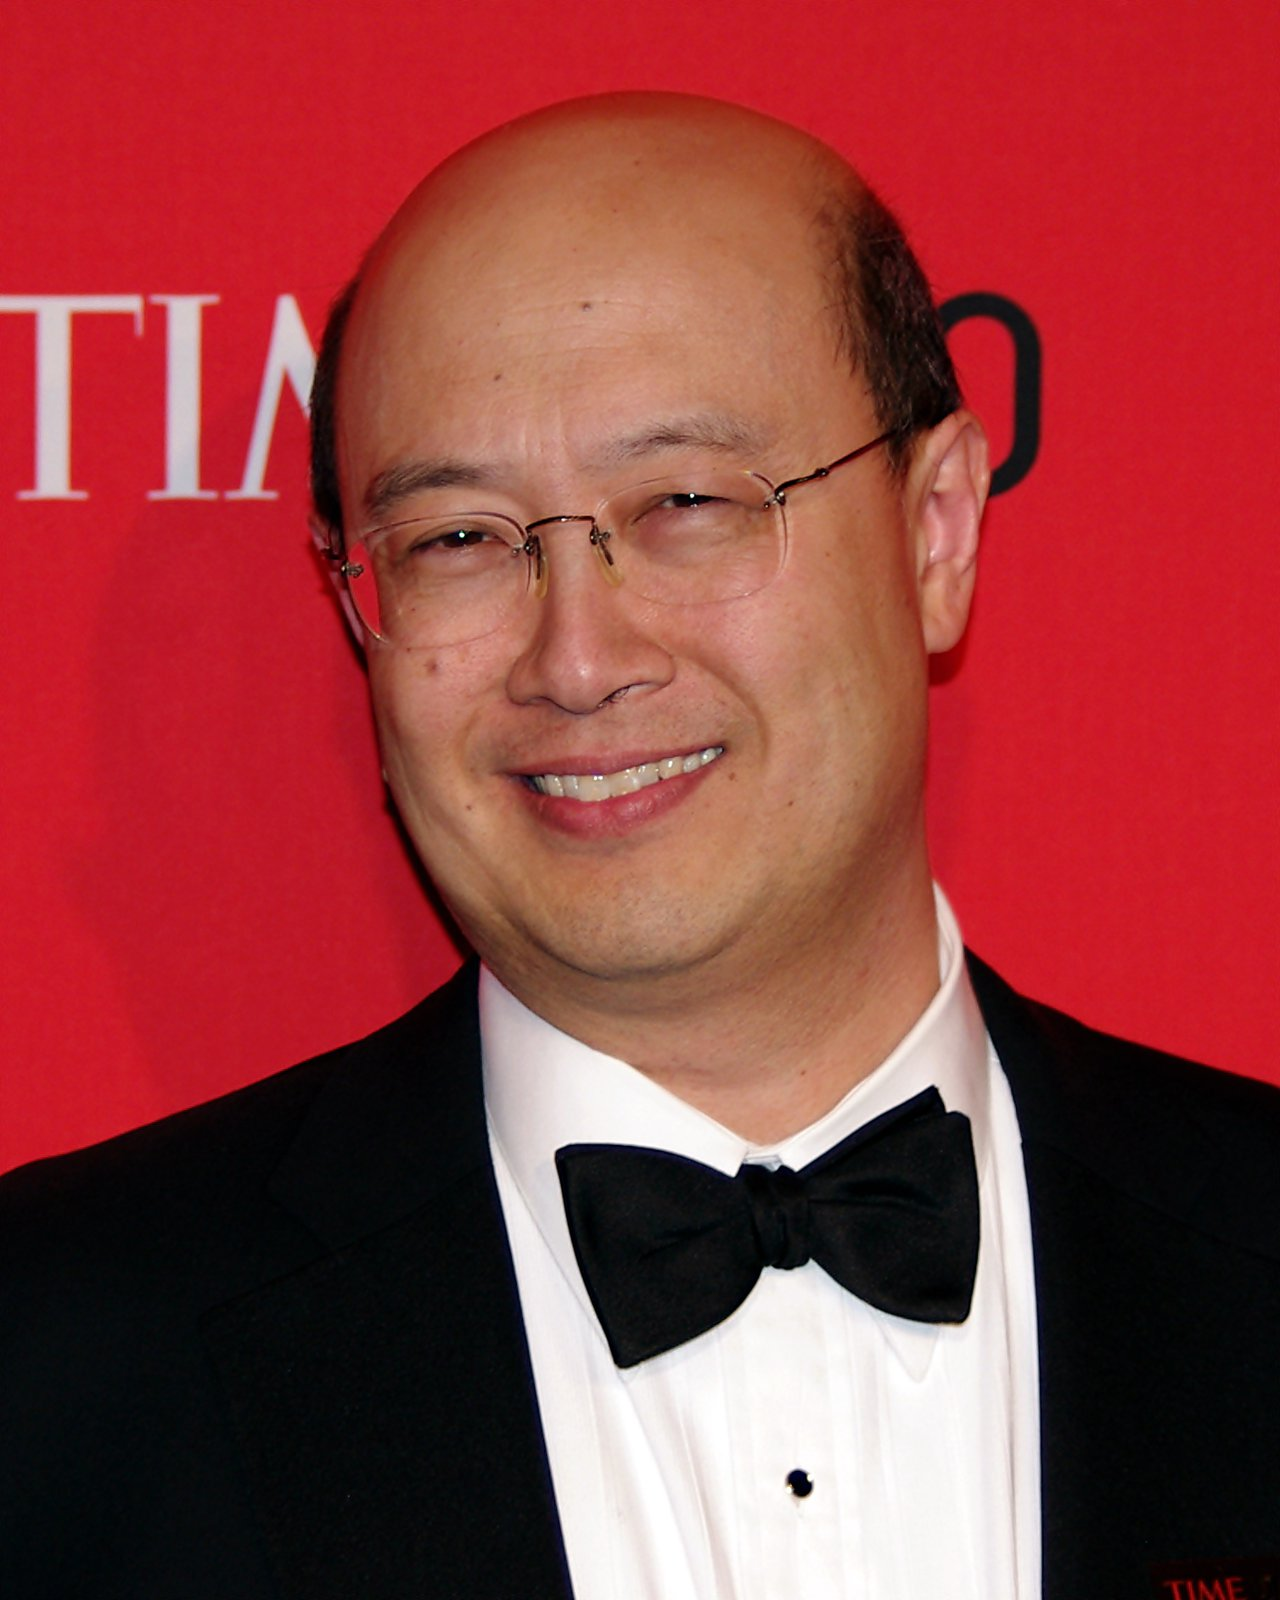
\includegraphics[height=0.40\textheight]{ch7_lo_2012.jpg}\\[1mm]
\imgcap{Andrew W. Lo, MIT}
\imgcredit{https://commons.wikimedia.org/wiki/File:Andrew_Lo_2012_Shankbone_2.JPG}{Photo: David Shankbone (2012); CC BY 3.0; Wikimedia Commons}
\end{column}
\end{columns}\sfmquantlet{Ch_07}{SFM_ch7_variance_ratio}
\end{frame}

\begin{frame}{Why the Robust Test: a Monte Carlo Check}
\itemsize{\footnotesize}
\begin{center}
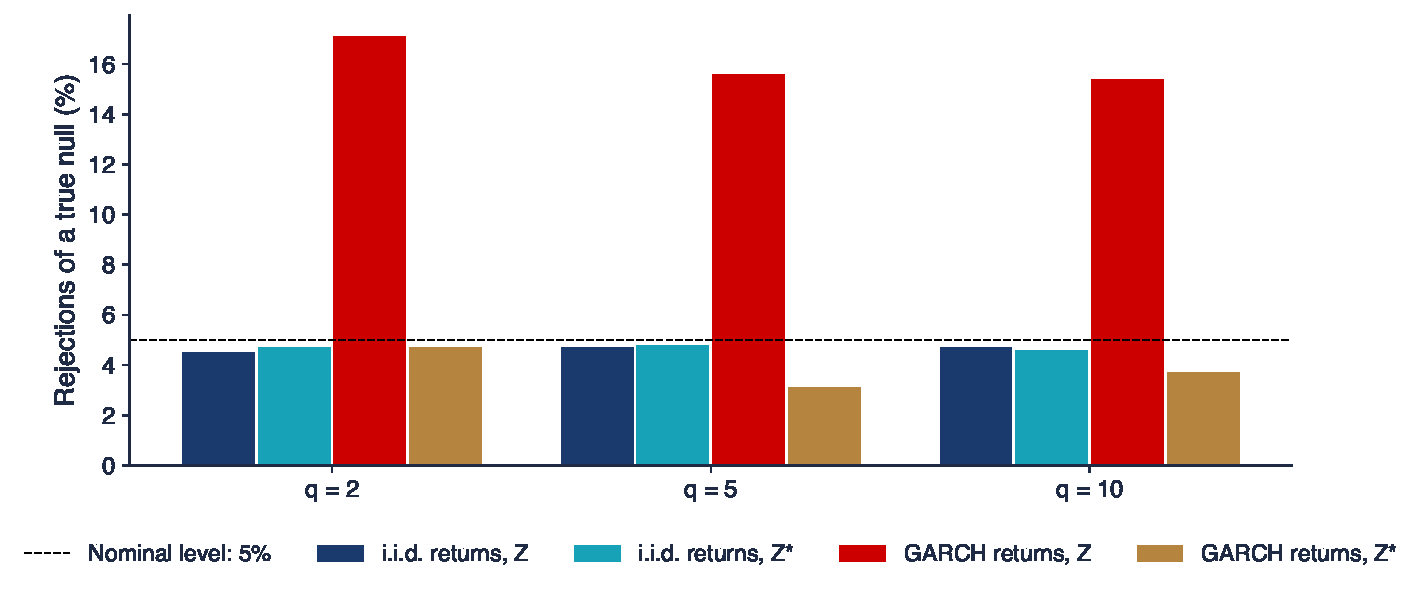
\includegraphics[width=0.97\textwidth,height=0.48\textheight,keepaspectratio]{sfm_ch7_vr_size.pdf}
\end{center}
\vspace{-0.25cm}
\begin{itemize}
    \item 1\,000 samples of $T = 2000$ returns with $H_0$ true: i.i.d.\ Normal, and GARCH(1,1) ($\alpha = 0.12$, $\beta = 0.86$): uncorrelated, with volatility clustering
    \item i.i.d.: both reject about 5\%; GARCH: $Z(2)$ rejects 17.1\% of the time, $Z^*(2)$ only 4.7\%
    \item The \textbf{size} of a test: how often it rejects a true $H_0$; $Z$ finds ``inefficiency'' that is only volatility clustering
\end{itemize}
\sfmquantlet{Ch_07}{SFM_ch7_variance_ratio}
\end{frame}

\begin{frame}{Variance Ratios for Horizons of 2 to 40 Days}
\itemsize{\footnotesize}
\begin{center}
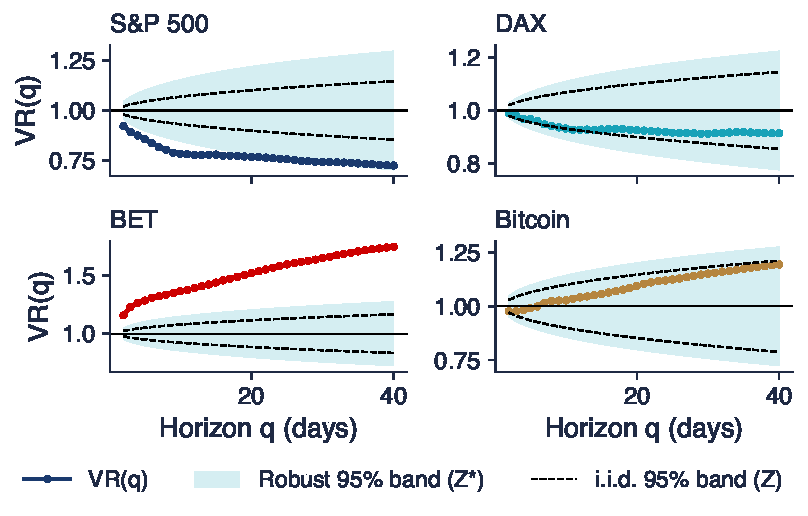
\includegraphics[width=0.97\textwidth,height=0.58\textheight,keepaspectratio]{sfm_ch7_vr_profile.pdf}
\end{center}
\vspace{-0.25cm}
\begin{itemize}
    \item S\&P 500: VR falls below 1 at every horizon (mean reversion); BET: VR rises up to about 1.517 at 20 days and beyond (momentum)
    \item DAX and Bitcoin: inside the robust band (shaded) at every horizon; the i.i.d.\ band (dashed) is much narrower
\end{itemize}
\sfmquantlet{Ch_07}{SFM_ch7_variance_ratio}
\end{frame}

\begin{frame}{Variance Ratios and Robust Tests}
\itemsize{\footnotesize}
\begin{center}
\scriptsize
\begin{tabular}{lrrrrrrrr}
\toprule
& VR(2) & VR(5) & VR(10) & VR(20) & $Z^*(2)$ & $Z^*(5)$ & $Z^*(10)$ & $Z^*(20)$ \\
\midrule
S\&P 500 & $0.922$ & $0.856$ & $0.783$ & $0.767$ & ${-3.37}$ & ${-2.76}$ & ${-2.73}$ & ${-2.06}$ \\
DAX & $0.990$ & $0.968$ & $0.932$ & $0.925$ & ${-0.61}$ & ${-0.88}$ & ${-1.21}$ & ${-0.91}$ \\
BET & $1.156$ & $1.283$ & $1.362$ & $1.517$ & ${5.99}$ & ${5.25}$ & ${4.74}$ & ${4.94}$ \\
Bitcoin & $0.977$ & $0.991$ & $1.027$ & $1.094$ & ${-0.88}$ & ${-0.19}$ & ${0.37}$ & ${0.91}$ \\
TLV & $1.009$ & $0.997$ & $0.954$ & $0.995$ & ${0.34}$ & ${-0.04}$ & ${-0.48}$ & ${-0.04}$ \\
SNP & $0.985$ & $0.960$ & $0.975$ & $1.038$ & ${-0.53}$ & ${-0.68}$ & ${-0.29}$ & ${0.32}$ \\
BRD & $1.032$ & $1.083$ & $1.078$ & $1.107$ & ${1.28}$ & ${1.55}$ & ${0.97}$ & ${0.96}$ \\
TGN & $1.055$ & $1.150$ & $1.142$ & $1.166$ & ${2.05}$ & ${2.60}$ & ${1.69}$ & ${1.44}$ \\
\bottomrule
\end{tabular}
\end{center}
\begin{itemize}
    \item $|Z^*| > 1.96$: reject the random walk at 5\% for that horizon
    \item S\&P 500: significant mean reversion at all four horizons; BET: significant momentum at all four
    \item Transgaz: $Z^*(2) = 2.05$ and $Z^*(5) = 2.60$; DAX, Bitcoin, TLV, SNP, BRD: no rejection
    \item But eight tests per series at once: some ``significant'' horizons appear by chance
\end{itemize}\sfmquantlet{Ch_07}{SFM_ch7_variance_ratio}
\end{frame}

\begin{frame}{Several Horizons at Once: the Chow--Denning Test}
\itemsize{\small}
\begin{itemize}
    \item Testing $q = 2, 5, 10, 20$ separately at 5\% gives a much higher chance of at least one false rejection
    \begin{itemize}
        \item for 4 independent tests: $1 - 0.95^4 = 18.5\%$
    \end{itemize}
    \item \textbf{CD} (Chow--Denning) statistic \refCD: $\mathrm{CD} = \max_{i} |Z^*(q_i)|$, $i = 1, \dots, m$
    \begin{itemize}
        \item critical value from the studentised maximum modulus law: $P(\mathrm{CD} \le c) = (2\Phi(c) - 1)^m$
        \item $m = 4$, 5\%: $c = 2.49$ instead of $1.96$; $\Phi$: the standard Normal distribution function
    \end{itemize}
    \item Reject the random walk if the largest $|Z^*|$ exceeds $2.49$: one decision for all horizons
\end{itemize}
\end{frame}

\begin{frame}{An Automatic Choice of the Horizon}
\itemsize{\small}
\begin{itemize}
    \item The horizon $q$ can be chosen from the data: the automatic VR test \refChoi
    \begin{itemize}
        \item $\mathrm{VR}(k) = 1 + 2\sum_{i=1}^{T-1} w(i/k)\,\hat\rho(i)$, with smoothly declining weights $w$ (quadratic spectral kernel) \refAndrews
        \item the bandwidth $k$ grows with the first-order autocorrelation and with $T$; statistic $\sqrt{T/k}\,(\mathrm{VR}(k) - 1)/\sqrt2 \approx N(0, 1)$
    \end{itemize}
    \item \textbf{Wild bootstrap} p-value \refKimB: resample $r_t^* = \eta_t(r_t - \bar r)$ with $\eta_t \sim N(0, 1)$, 500 times
    \begin{itemize}
        \item each $r_t^*$ keeps the size of $r_t$ (its volatility) but loses any autocorrelation: a robust null distribution
    \end{itemize}
    \item Three tools, one question: $Z^*(q)$ for a chosen horizon, CD for a set of horizons, the automatic test for a horizon chosen by the data
\end{itemize}
\end{frame}

\begin{frame}{Joint and Automatic Tests on Real Data}
\itemsize{\footnotesize}
\begin{center}
\scriptsize
\begin{tabular}{lrrrrrr}
\toprule
& $T$ & CD & p & $\hat k$ & automatic VR & p (bootstrap) \\
\midrule
S\&P 500 & 9\,240 & $3.37$ & 0.003 & $3.7$ & ${-5.21}$ & 0.006 \\
DAX & 9\,288 & $1.21$ & 0.644 & $1.7$ & ${-0.39}$ & 0.608 \\
BET & 7\,243 & $5.99$ & $<$\,0.001 & $5.6$ & ${8.86}$ & $<$\,0.001 \\
Bitcoin & 4\,384 & $0.91$ & 0.835 & $2.0$ & ${-1.01}$ & 0.352 \\
TLV & 3\,788 & $0.48$ & 0.981 & $1.5$ & ${0.31}$ & 0.718 \\
SNP & 3\,815 & $0.68$ & 0.937 & $1.7$ & ${-0.53}$ & 0.562 \\
BRD & 3\,771 & $1.55$ & 0.403 & $2.3$ & ${1.58}$ & 0.152 \\
TGN & 3\,725 & $2.60$ & 0.037 & $3.0$ & ${3.78}$ & 0.004 \\
\bottomrule
\end{tabular}
\end{center}
\begin{itemize}
    \item Both tests reject for the S\&P 500, the BET and Transgaz; neither rejects for DAX, Bitcoin, TLV, SNP and BRD
    \item $\hat k$ is large where the first autocorrelation is large (BET $5.6$), small where it is near 0 (DAX $1.7$)
    \item Interpretation: rejection does not mean profit: an autocorrelation of $-0.079$ predicts less than 1\% of the variance of tomorrow's return; trading costs absorb most of it
\end{itemize}\sfmquantlet{Ch_07}{SFM_ch7_variance_ratio}
\end{frame}

\begin{frame}{Recap: The Variance-Ratio Test}
\itemsize{\small}
\begin{itemize}
    \item $\mathrm{VR}(q) = 1 + 2\sum_{k<q}(1 - k/q)\rho(k)$; $> 1$ momentum, $< 1$ mean reversion
    \item Use $Z^*(q)$: the homoskedastic $Z(q)$ over-rejects under volatility clustering
    \item Several horizons: Chow--Denning; data-driven horizon: automatic VR with wild bootstrap
    \item S\&P 500 mean-reverting, BET trending; DAX, Bitcoin and most BVB stocks consistent with a random walk
\end{itemize}
\end{frame}


%=============================================================================
\section{Efficiency across Markets and over Time}
%=============================================================================

\begin{frame}{Sixteen Markets over the Last Ten Years}
\itemsize{\footnotesize}
\begin{center}
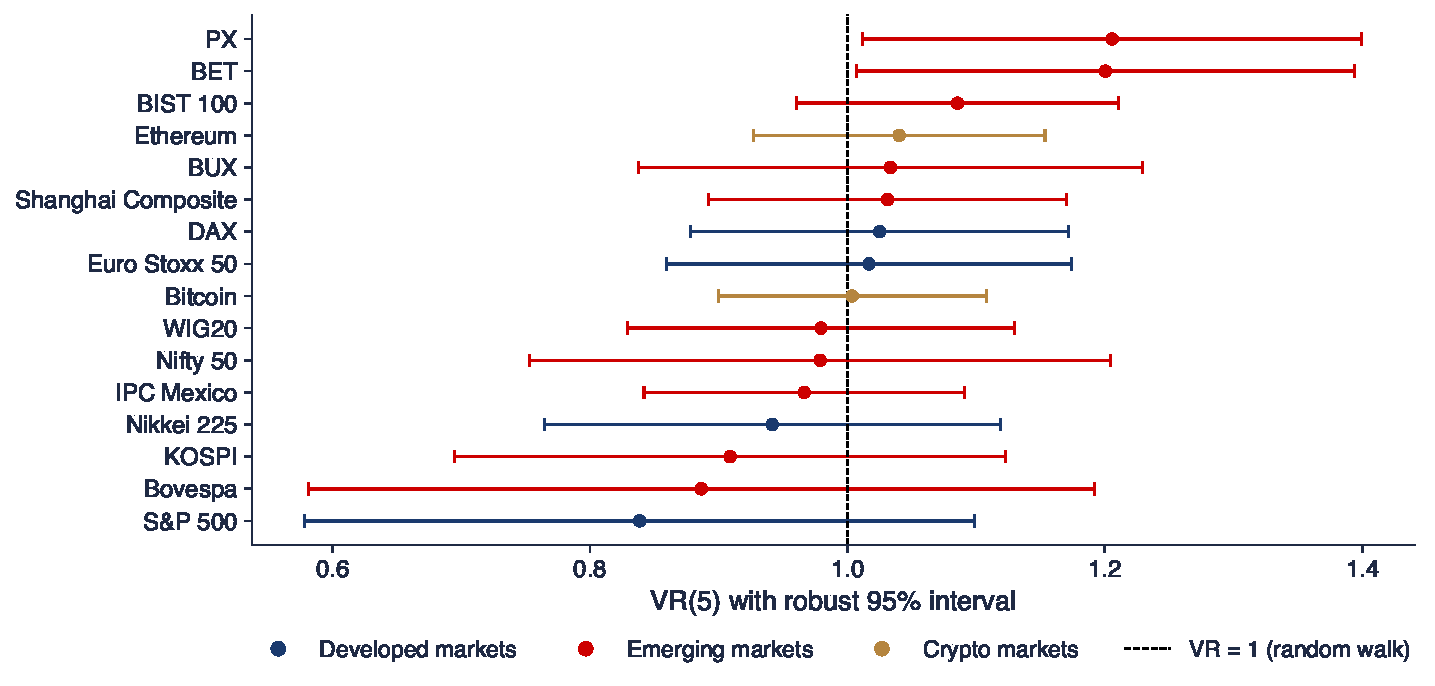
\includegraphics[width=0.97\textwidth,height=0.64\textheight,keepaspectratio]{sfm_ch7_vr_markets.pdf}
\end{center}
\vspace{-0.25cm}
\begin{itemize}
    \item VR(5) with its robust 95\% interval, from 19 September 2016 to 18 September 2026: developed, emerging and crypto markets
\end{itemize}
\sfmquantlet{Ch_07}{SFM_ch7_markets_efficiency}
\end{frame}

\begin{frame}{Reading the Cross-Market Comparison}
\itemsize{\small}
\begin{itemize}
    \item Only two intervals exclude 1: the PX ($Z^*(5) = 2.08$) and the BET ($Z^*(5) = 2.03$), both above 1
    \begin{itemize}
        \item two smaller Central European markets, with less liquid index stocks
    \end{itemize}
    \item \textbf{Many markets, many tests}: 16 tests at 5\% give 0.8 false rejections on average
    \begin{itemize}
        \item if the tests were independent, the chance of at least one false rejection would be $1 - 0.95^{16} = 56\%$
        \item Chow--Denning over four horizons: no market rejects at 5\% (BET p = 0.159, PX p = 0.142)
    \end{itemize}
    \item S\&P 500: VR(5) $= 0.84$, the lowest, but with a wide interval ($Z^* = -1.22$): the large swings of 2020 inflate $\hat\theta$
    \item Bitcoin and Ethereum: VR(5) close to 1, as for developed markets
\end{itemize}\sfmquantlet{Ch_07}{SFM_ch7_markets_efficiency}
\end{frame}

\begin{frame}{The Adaptive Markets Hypothesis}
\itemsize{\small}
\begin{columns}[T]
\begin{column}{0.62\textwidth}
\begin{itemize}
    \item \textbf{AMH} (adaptive markets hypothesis) \refLo: markets are ecosystems of traders who learn and adapt
    \begin{itemize}
        \item profit opportunities appear, are exploited and disappear; efficiency changes with the environment
        \item crises, new technology, new participants and regulation move the market away from efficiency or back towards it
    \end{itemize}
    \item Testable consequence: predictability varies over time
    \begin{itemize}
        \item evidence: \refKSL{} (U.S., a century of data); \refUM; survey: \refLB
    \end{itemize}
    \item Tool: the same test on rolling windows
\end{itemize}
\end{column}
\begin{column}{0.34\textwidth}
\centering
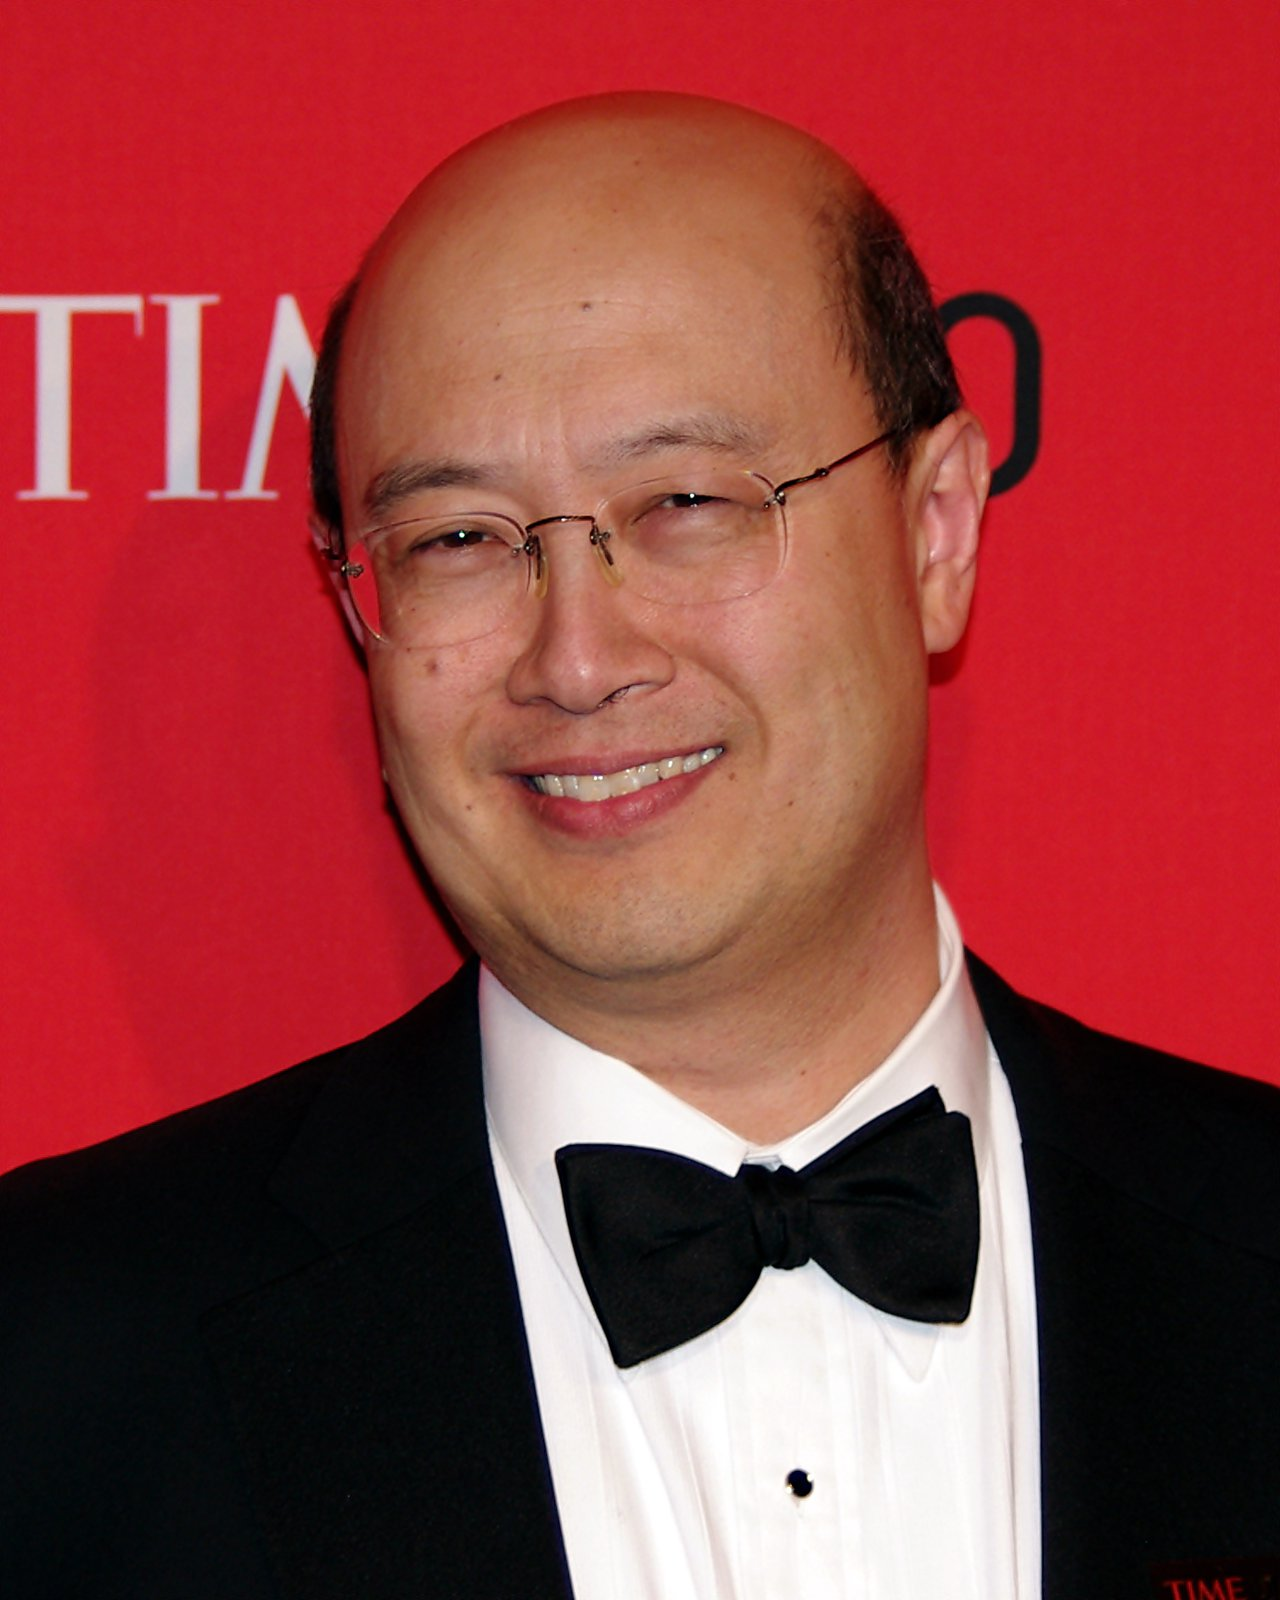
\includegraphics[height=0.42\textheight]{ch7_lo_2012.jpg}\\[1mm]
\imgcap{Andrew W. Lo, author of the AMH}
\imgcredit{https://commons.wikimedia.org/wiki/File:Andrew_Lo_2012_Shankbone_2.JPG}{Photo: David Shankbone (2012); CC BY 3.0; Wikimedia Commons}
\end{column}
\end{columns}
\end{frame}

\begin{frame}{Rolling Variance Ratios}
\itemsize{\footnotesize}
\begin{center}
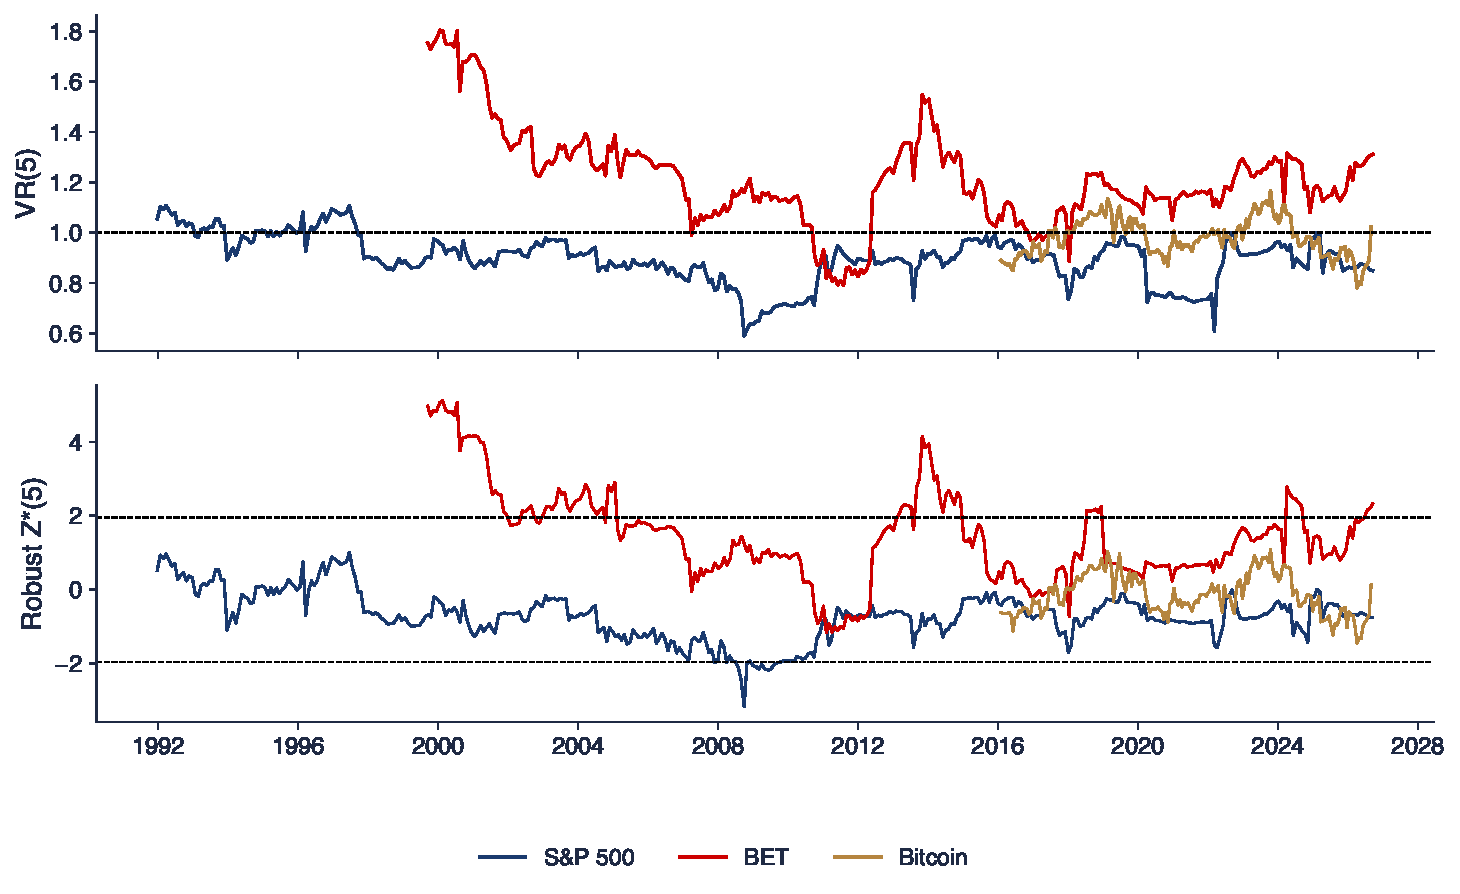
\includegraphics[width=0.97\textwidth,height=0.64\textheight,keepaspectratio]{sfm_ch7_rolling_vr.pdf}
\end{center}
\vspace{-0.25cm}
\begin{itemize}
    \item VR(5) and $Z^*(5)$ on windows of 500 trading days (about two years), a new window every 21 days, dated at the window end
\end{itemize}
\sfmquantlet{Ch_07}{SFM_ch7_adaptive_markets}
\end{frame}

\begin{frame}{Reading the Rolling Variance Ratios}
\itemsize{\small}
\begin{itemize}
    \item BET: VR(5) up to 1.80 in the window ending in 2000; closer to 1 after 2008, apart from short episodes
    \begin{itemize}
        \item 29\% of the windows reject at 5\%, all of them with VR $> 1$ (momentum)
    \end{itemize}
    \item S\&P 500: VR(5) mostly below 1; the lowest, 0.59, in the window ending in 2008
    \begin{itemize}
        \item 4\% of the windows reject, all with VR $< 1$: reversals are strongest in crises
    \end{itemize}
    \item Bitcoin: no window rejects since 2016 (185 windows)
    \item Caution: consecutive windows share 479 of 500 days; the share of rejecting windows is a description, not a test
\end{itemize}\sfmquantlet{Ch_07}{SFM_ch7_adaptive_markets}
\end{frame}

\begin{frame}{Three Sub-Periods per Market}
\itemsize{\footnotesize}
\begin{center}
\scriptsize
\begin{tabular}{llrrrrr}
\toprule
& period & $T$ & $\hat\rho(1)$ & VR(5) & $Z^*(5)$ & CD p \\
\midrule
BET & 1997--2006 & 2\,306 & ${0.270}$ & $1.50$ & ${6.15}$ & $<$\,0.001 \\
BET & 2007--2016 & 2\,516 & ${0.066}$ & $1.08$ & ${0.82}$ & 0.262 \\
BET & 2017--2026 & 2\,421 & ${0.064}$ & $1.20$ & ${2.04}$ & 0.154 \\
S\&P 500 & 1990--2001 & 3\,025 & ${0.017}$ & $0.96$ & ${-0.62}$ & 0.334 \\
S\&P 500 & 2002--2013 & 3\,019 & ${-0.100}$ & $0.80$ & ${-2.53}$ & 0.010 \\
S\&P 500 & 2014--2026 & 3\,196 & ${-0.124}$ & $0.85$ & ${-1.30}$ & 0.080 \\
Bitcoin & 2014--2017 & 1\,201 & ${0.028}$ & $0.98$ & ${-0.23}$ & 0.983 \\
Bitcoin & 2018--2021 & 1\,461 & ${-0.058}$ & $0.98$ & ${-0.21}$ & 0.374 \\
Bitcoin & 2022--2026 & 1\,722 & ${-0.026}$ & $1.01$ & ${0.18}$ & 0.924 \\
\bottomrule
\end{tabular}
\end{center}
\begin{itemize}
    \item BET: strong momentum in 1997--2006 ($\hat\rho(1) = 0.270$), much weaker afterwards; since 2017 VR(5) is still above 1, but the joint test does not reject
    \item S\&P 500: the negative autocorrelation appears after 2002; Bitcoin: no rejection in any period since 2014; \refUrquhart{} found inefficiency in its earliest years
\end{itemize}\sfmquantlet{Ch_07}{SFM_ch7_adaptive_markets}
\end{frame}

\begin{frame}{Why the Early BET Was Predictable}
\itemsize{\small}
\begin{columns}[T]
\begin{column}{0.60\textwidth}
\begin{itemize}
    \item \textbf{Thin trading}: few trades per day in many index stocks
    \begin{itemize}
        \item a closing price may be hours old; news enters the index over several days
        \item the index then shows positive autocorrelation even if each stock is efficient
    \end{itemize}
    \item Changes after 2007
    \begin{itemize}
        \item more liquidity, foreign investors, EU membership, the FTSE Russell upgrade to Secondary Emerging (2020) \refFTSE
    \end{itemize}
    \item Crashes on the Bucharest Stock Exchange: \refPeleA
\end{itemize}
\end{column}
\begin{column}{0.36\textwidth}
\centering
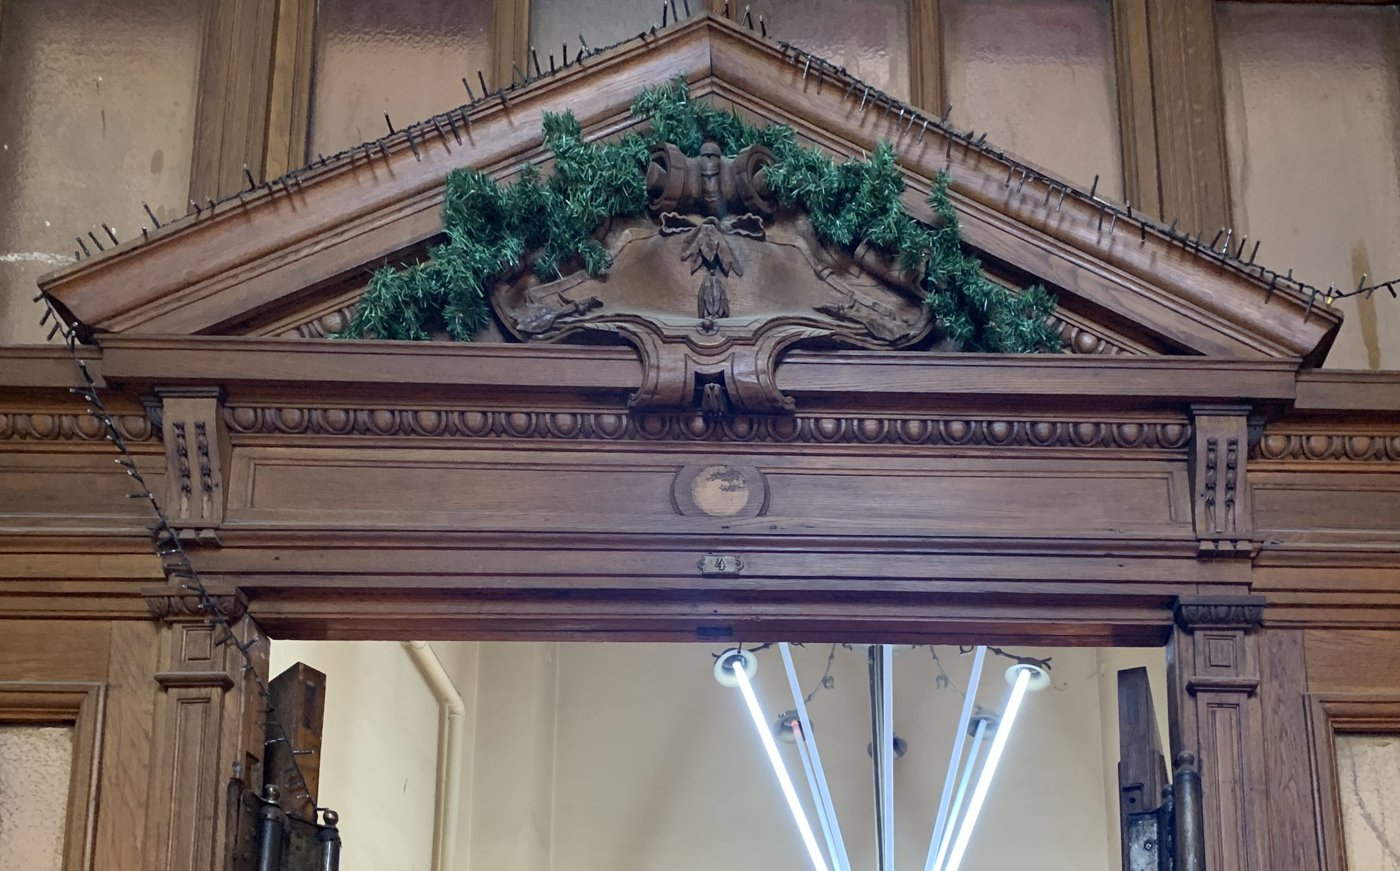
\includegraphics[height=0.32\textheight]{ch5_bvb_palace_2019.jpg}\\[1mm]
\imgcap{The Stock Exchange Palace, Bucharest}
\imgcredit{https://commons.wikimedia.org/wiki/File:Stock_Exchange_Palace_(Bucharest).jpg}{Photo: Neoclassicism Enthusiast (2019); CC BY-SA 4.0; Wikimedia Commons}
\end{column}
\end{columns}
\end{frame}

\begin{frame}{Recap: Efficiency across Markets and over Time}
\itemsize{\small}
\begin{itemize}
    \item Over the last ten years most markets, including Bitcoin, are consistent with a random walk
    \item Efficiency changes over time: the AMH; rolling windows show it, but overlap
    \item The early BET: thin trading and momentum; today: much closer to a random walk
    \item Many markets, many tests: expect some false rejections
\end{itemize}
\end{frame}


%=============================================================================
\section{Semi-Strong Form, Strong Form and Anomalies}
%=============================================================================

\begin{frame}{Event Studies and the Strong Form}
\itemsize{\small}
\begin{itemize}
    \item \textbf{Event study} (semi-strong form) \refMacKinlay, \refCLM, Ch.~4: how fast does a price absorb public news?
    \begin{itemize}
        \item abnormal return: the return minus the return of a model (for example the market); cumulated over a window around the announcement
        \item efficient: a jump on the day of the news, no drift afterwards
        \item recent research: how fast futures prices absorb news, measured in nanoseconds at Eurex and CME \refPeleB; market responses to Ethereum upgrades \refPeleC
    \end{itemize}
    \item \textbf{Strong form}: can anyone with private information earn excess returns?
    \begin{itemize}
        \item insiders (managers trading their own shares) do: insider trading is illegal for this reason
        \item professional fund managers mostly do not \refJensen, \refFF
    \end{itemize}
\end{itemize}
\end{frame}

\begin{frame}{Calendar Anomalies}
\itemsize{\small}
\begin{itemize}
    \item An \textbf{anomaly}: a pattern in returns that the equilibrium model does not explain
    \begin{itemize}
        \item \textbf{weekend effect}: low or negative Monday returns \refFrench
        \item \textbf{January effect}: higher returns in January, mostly for small stocks \refRK
        \item \textbf{turn-of-the-month effect}: returns concentrated around the first trading days of the month \refAriel
    \end{itemize}
    \item Do anomalies last?
    \begin{itemize}
        \item returns of published anomalies fall after publication: traders learn \refMP
        \item hundreds of patterns have been tested: a new one needs $|t| > 3$, not 2 \refHLZ
    \end{itemize}
    \item Data mining: with enough calendar splits, some will look significant by chance
\end{itemize}
\end{frame}

\begin{frame}{Day-of-Week Returns: S\&P 500 and BET}
\itemsize{\footnotesize}
\begin{center}
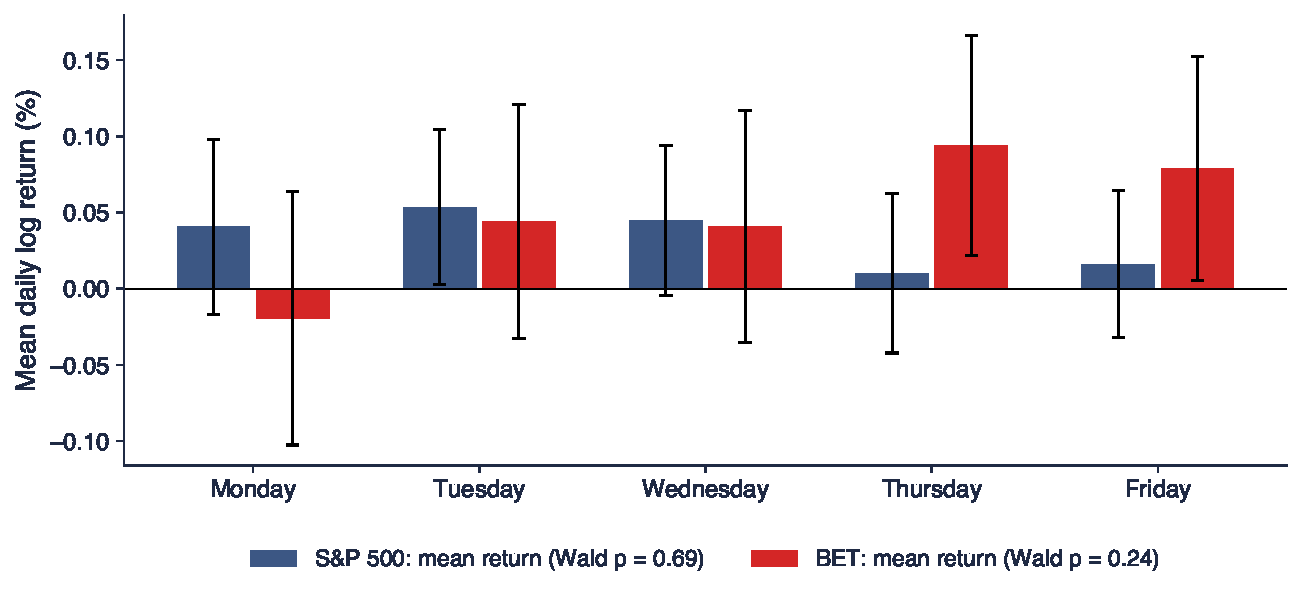
\includegraphics[width=0.97\textwidth,height=0.50\textheight,keepaspectratio]{sfm_ch7_calendar.pdf}
\end{center}
\vspace{-0.25cm}
\begin{itemize}
    \item Mean daily return by weekday with 95\% intervals (Newey--West standard errors \refNW); Wald test of equal means: S\&P 500 p = 0.69, BET p = 0.24
    \item BET Monday: $-0.019\%$, the only negative mean, yet not significant; January: BET $0.185\%$ per day against $0.036\%$ ($t = 1.72$, p = 0.09); S\&P 500: p = 0.59
    \item No calendar effect survives at 5\% in our data
\end{itemize}
\sfmquantlet{Ch_07}{SFM_ch7_calendar_anomalies}
\end{frame}

\begin{frame}{Recap: Semi-Strong Form, Strong Form and Anomalies}
\itemsize{\small}
\begin{itemize}
    \item Event studies: prices react to public news at once, with no drift, in efficient markets
    \item Strong form fails for insiders, holds roughly for professional managers
    \item Calendar anomalies: weak in our data, and they fade after publication
\end{itemize}
\end{frame}


%=============================================================================
\section{AI for Scientific Discovery}
%=============================================================================

\begin{frame}{An Open Question}
\itemsize{\small}
\begin{itemize}
    \item \textbf{Did the BET become more efficient after Romania's upgrade to Secondary Emerging market (September 2020)?} \refFTSE
    \begin{itemize}
        \item five years before: $\hat\rho(1) = -0.002$, VR(5) $= 1.12$ ($Z^* = 0.80$); five years after: $\hat\rho(1) = 0.087$, VR(5) $= 1.18$ ($Z^* = 1.78$)
        \item difference of the two VR(5): $z = 0.34$: no evidence of a change
    \end{itemize}
    \item Why it is open: COVID-19, new large listings and higher volumes happened at the same time; is the index or each stock the right unit?
    \item AI tools can speed up such a study; they do not replace checking it \refWang
\end{itemize}\sfmquantlet{Ch_07}{SFM_ch7_adaptive_markets}
\end{frame}

\begin{frame}{How AI Could Help}
\itemsize{\small}
\begin{itemize}
    \item \textbf{Literature}: list studies of efficiency in Central and Eastern European markets and the tests they use
    \item \textbf{Code}: a first draft of rolling Lo--MacKinlay and automatic VR tests for BET stocks, with wild-bootstrap p-values
    \item \textbf{Robustness}: other windows, other horizons, BET-TR instead of BET, trading volume as a control
    \item Example prompt
    \begin{itemize}
        \item \aiprompt{Write a Python function that computes the Lo-MacKinlay variance ratio VR(5) and the heteroskedasticity-robust z-statistic for daily BET log returns on rolling 500-day windows, and test whether the mean VR differs before and after 21 September 2020.}
    \end{itemize}
\end{itemize}
\end{frame}

\begin{frame}{What to Check}
\itemsize{\small}
\begin{itemize}
    \item The statistic: robust $Z^*$, not the homoskedastic $Z$; a draft that uses $Z$ will ``find'' inefficiency
    \item Log returns of the index, not price levels; no unit-root test on returns used as an efficiency test
    \item Rolling windows overlap: a $t$-test on the mean of rolling statistics treats dependent numbers as independent
    \item The event date and the window are fixed before looking at the result
    \item References: every cited paper must exist; check the DOI
\end{itemize}
\end{frame}

\begin{frame}{Project Idea}
\itemsize{\small}
\begin{itemize}
    \item \textbf{Question}: is the Bucharest market more efficient today than in 2015?
    \begin{itemize}
        \item a second question: does the change appear in the index or in the individual stocks?
        \item data: BET since 1997, BET-TR since 2014, BVB stocks (TLV, SNP, BRD, TGN) since 2010 (EODHD)
    \end{itemize}
    \item Steps
    \begin{itemize}
        \item rolling VR(2), VR(5) with $Z^*$ and the Chow--Denning test for the index and for each stock
        \item compare 2015--2020 with 2020--2025 by a block bootstrap of the difference
        \item repeat for the WIG20 and the BUX as controls: did all of them change at the same time?
    \end{itemize}
    \item Deliverable: one table, one chart, and a paragraph on what the data can and cannot show
    \item Declare any AI use, and list the errors of the AI that you corrected
\end{itemize}
\end{frame}


%=============================================================================
\section{Summary}
%=============================================================================

\begin{frame}{Key Takeaways}
\itemsize{\small}
\begin{itemize}
    \item Efficient market: prices reflect information; weak form = past prices cannot be used to earn excess returns
    \item The right null is the martingale (RW3), not RW1: volatility clustering is not inefficiency
    \item Log prices are $I(1)$ and returns $I(0)$ in all our series; a unit root alone does not prove efficiency
    \item Use robust tests: $\tilde Q$ and $Z^*(q)$; join horizons with Chow--Denning or let the data choose (automatic VR)
    \item Evidence: S\&P 500 slightly mean-reverting, early BET trending, most markets close to efficient today; efficiency varies over time
    \item Statistical predictability is not profit: costs and risk decide
\end{itemize}
\end{frame}

\begin{frame}{Key Formulas}
\itemsize{\small}
{\renewcommand{\arraystretch}{1.45}\begin{center}
\scriptsize
\begin{tabular}{ll}
\toprule
\textbf{Quantity} & \textbf{Formula} \\
\midrule
Random walk & $p_t = \mu + p_{t-1} + \varepsilon_t$, \quad $\mathrm{Var}(r_t(q)) = q\sigma^2$ \\
Sample ACF & $\hat\rho(k) = \sum_t e_te_{t-k}/\sum_t e_t^2$, \quad band $\pm 1.96\sqrt{\hat\delta(k)/T}$ \\
Ljung--Box & $Q_{LB}(m) = T(T+2)\sum_{k=1}^m \hat\rho(k)^2/(T-k) \sim \chi^2(m)$ \\
Runs test & $E[R] = 2n_1n_2/n + 1$, \quad $z = (R - E[R])/\mathrm{sd}(R)$ \\
ADF & $\Delta p_t = c + bt + \gamma p_{t-1} + \sum_j \delta_j\Delta p_{t-j} + \varepsilon_t$, \quad $\tau = \hat\gamma/\mathrm{SE}(\hat\gamma)$ \\
KPSS & $\sum_t S_t^2/(T^2\hat\lambda^2)$, \quad $H_0$: stationarity \\
VR & $\mathrm{VR}(q) = 1 + 2\sum_{k=1}^{q-1}(1 - k/q)\rho(k)$ \\
Robust VR test & $Z^*(q) = (\widehat{\mathrm{VR}}(q) - 1)/\sqrt{\hat\theta(q)/T}$, \quad $\hat\theta(q) = \sum_{j<q}[2(q-j)/q]^2\hat\delta(j)$ \\
Chow--Denning & $\max_i |Z^*(q_i)|$, \quad $P(\mathrm{CD} \le c) = (2\Phi(c) - 1)^m$ \\
\bottomrule
\end{tabular}
\end{center}
}
\end{frame}

\begin{frame}{Check Yourself}
\itemsize{\small}
\begin{itemize}
    \item \textbf{Question}: $\hat\rho(1) = 0.10$ and $\hat\rho(k) = 0$ for $k \ge 2$; what does VR(2) tell us?
    \begin{itemize}
        \item \textbf{Answer}: $1 + 0.10 = 1.10$: the two-day variance is 10\% larger than under a random walk: momentum
    \end{itemize}
    \item \textbf{Question}: ADF does not reject on log prices and KPSS rejects; is the market efficient?
    \begin{itemize}
        \item \textbf{Answer}: we only know that prices are $I(1)$; efficiency needs tests on the increments (ACF, VR)
    \end{itemize}
    \item \textbf{Question}: $Q_{LB}(10)$ rejects strongly for squared returns; is weak-form efficiency rejected?
    \begin{itemize}
        \item \textbf{Answer}: no; this is volatility clustering; it rejects RW1 and RW2, not the martingale
    \end{itemize}
    \item Next: \sfmchlink{https://danpele.github.io/SFM/EN/Courses/chapter8_volatility_estimators.pdf}{Chapter 8}, volatility estimators and volatility clustering
\end{itemize}
\end{frame}


%=============================================================================
\section{References}
%=============================================================================

\begin{frame}{References (1/3)}
\itemsize{\tiny}
\begin{itemize}
    \item Andrews, D.W.K. (1991). \href{https://doi.org/10.2307/2938229}{Heteroskedasticity and autocorrelation consistent covariance matrix estimation}. \textit{Econometrica}, 59(3), 817--858.
    \item Ariel, R.A. (1987). \href{https://doi.org/10.1016/0304-405X(87)90066-3}{A monthly effect in stock returns}. \textit{Journal of Financial Economics}, 18(1), 161--174.
    \item Bachelier, L. (1900). \href{https://doi.org/10.24033/asens.476}{Théorie de la spéculation}. \textit{Annales scientifiques de l'École normale supérieure}, 17, 21--86.
    \item Borak, S., Härdle, W.K., López-Cabrera, B. (2013). \href{https://doi.org/10.1007/978-3-642-33929-5}{\textit{Statistics of Financial Markets: Exercises and Solutions}}, 2nd ed. Springer.
    \item Box, G.E.P., Pierce, D.A. (1970). \href{https://doi.org/10.1080/01621459.1970.10481180}{Distribution of residual autocorrelations in autoregressive-integrated moving average time series models}. \textit{Journal of the American Statistical Association}, 65(332), 1509--1526.
    \item Campbell, J.Y., Lo, A.W., MacKinlay, A.C. (1997). \href{https://doi.org/10.1515/9781400830213}{\textit{The Econometrics of Financial Markets}}. Princeton University Press.
    \item Choi, I. (1999). \href{https://doi.org/10.1002/(SICI)1099-1255(199905/06)14:3<293::AID-JAE503>3.0.CO;2-5}{Testing the random walk hypothesis for real exchange rates}. \textit{Journal of Applied Econometrics}, 14(3), 293--308.
    \item Chow, K.V., Denning, K.C. (1993). \href{https://doi.org/10.1016/0304-4076(93)90051-6}{A simple multiple variance ratio test}. \textit{Journal of Econometrics}, 58(3), 385--401.
    \item Dickey, D.A., Fuller, W.A. (1979). \href{https://doi.org/10.1080/01621459.1979.10482531}{Distribution of the estimators for autoregressive time series with a unit root}. \textit{Journal of the American Statistical Association}, 74(366), 427--431.
    \item Escanciano, J.C., Lobato, I.N. (2009). \href{https://doi.org/10.1016/j.jeconom.2009.03.001}{An automatic Portmanteau test for serial correlation}. \textit{Journal of Econometrics}, 151(2), 140--149.
    \item Fama, E.F. (1965). \href{https://doi.org/10.1086/294743}{The behavior of stock-market prices}. \textit{Journal of Business}, 38(1), 34--105.
    \item Fama, E.F. (1970). \href{https://doi.org/10.1111/j.1540-6261.1970.tb00518.x}{Efficient capital markets: a review of theory and empirical work}. \textit{Journal of Finance}, 25(2), 383--417.
    \item Fama, E.F. (1991). \href{https://doi.org/10.1111/j.1540-6261.1991.tb04636.x}{Efficient capital markets: II}. \textit{Journal of Finance}, 46(5), 1575--1617.
    \item Fama, E.F., French, K.R. (2010). \href{https://doi.org/10.1111/j.1540-6261.2010.01598.x}{Luck versus skill in the cross-section of mutual fund returns}. \textit{Journal of Finance}, 65(5), 1915--1947.
    \item Franke, J., Härdle, W.K., Hafner, C.M. (2019). \href{https://doi.org/10.1007/978-3-030-13751-9}{\textit{Statistics of Financial Markets: An Introduction}}, 5th ed. Springer.
    \item French, K.R. (1980). \href{https://doi.org/10.1016/0304-405X(80)90021-5}{Stock returns and the weekend effect}. \textit{Journal of Financial Economics}, 8(1), 55--69.
\end{itemize}
\end{frame}

\begin{frame}{References (2/3)}
\itemsize{\tiny}
\begin{itemize}
    \item FTSE Russell (2019). \href{https://www.lseg.com/en/media-centre/press-releases/ftse-russell/2019/ftse-russell-announces-results-country-classification-review-equities-and-fixed-income}{FTSE Russell announces results of country classification review}. Press release, London Stock Exchange Group.
    \item Granger, C.W.J., Newbold, P. (1974). \href{https://doi.org/10.1016/0304-4076(74)90034-7}{Spurious regressions in econometrics}. \textit{Journal of Econometrics}, 2(2), 111--120.
    \item Grossman, S.J., Stiglitz, J.E. (1980). \href{https://ideas.repec.org/a/aea/aecrev/v70y1980i3p393-408.html}{On the impossibility of informationally efficient markets}. \textit{American Economic Review}, 70(3), 393--408.
    \item Harvey, C.R., Liu, Y., Zhu, H. (2016). \href{https://doi.org/10.1093/rfs/hhv059}{\ldots and the cross-section of expected returns}. \textit{Review of Financial Studies}, 29(1), 5--68.
    \item Jensen, M.C. (1968). \href{https://doi.org/10.1111/j.1540-6261.1968.tb00815.x}{The performance of mutual funds in the period 1945--1964}. \textit{Journal of Finance}, 23(2), 389--416.
    \item Kendall, M.G. (1953). \href{https://doi.org/10.2307/2980947}{The analysis of economic time-series, Part I: prices}. \textit{Journal of the Royal Statistical Society, Series A}, 116(1), 11--34.
    \item Kim, J.H. (2009). \href{https://doi.org/10.1016/j.frl.2009.04.003}{Automatic variance ratio test under conditional heteroskedasticity}. \textit{Finance Research Letters}, 6(3), 179--185.
    \item Kim, J.H., Shamsuddin, A., Lim, K.-P. (2011). \href{https://doi.org/10.1016/j.jempfin.2011.08.002}{Stock return predictability and the adaptive markets hypothesis: evidence from century-long U.S. data}. \textit{Journal of Empirical Finance}, 18(5), 868--879.
    \item Kwiatkowski, D., Phillips, P.C.B., Schmidt, P., Shin, Y. (1992). \href{https://doi.org/10.1016/0304-4076(92)90104-Y}{Testing the null hypothesis of stationarity against the alternative of a unit root}. \textit{Journal of Econometrics}, 54(1--3), 159--178.
    \item Lim, K.-P., Brooks, R. (2011). \href{https://doi.org/10.1111/j.1467-6419.2009.00611.x}{The evolution of stock market efficiency over time: a survey of the empirical literature}. \textit{Journal of Economic Surveys}, 25(1), 69--108.
    \item Lin, Y., Găman, A., Wang, Y., Pele, D.T. (2025). \href{https://doi.org/10.2139/ssrn.5176758}{Market responses to Ethereum development milestones: an event study approach}. SSRN Working Paper 5176758.
    \item Ljung, G.M., Box, G.E.P. (1978). \href{https://doi.org/10.1093/biomet/65.2.297}{On a measure of lack of fit in time series models}. \textit{Biometrika}, 65(2), 297--303.
    \item Lo, A.W. (2004). \href{https://doi.org/10.3905/jpm.2004.442611}{The adaptive markets hypothesis}. \textit{Journal of Portfolio Management}, 30(5), 15--29.
    \item Lo, A.W. (2017). \href{https://doi.org/10.1515/9781400887767}{\textit{Adaptive Markets: Financial Evolution at the Speed of Thought}}. Princeton University Press.
    \item Lo, A.W., MacKinlay, A.C. (1988). \href{https://doi.org/10.1093/rfs/1.1.41}{Stock market prices do not follow random walks: evidence from a simple specification test}. \textit{Review of Financial Studies}, 1(1), 41--66.
    \item MacKinlay, A.C. (1997). \href{https://ideas.repec.org/a/aea/jeclit/v35y1997i1p13-39.html}{Event studies in economics and finance}. \textit{Journal of Economic Literature}, 35(1), 13--39.
\end{itemize}
\end{frame}

\begin{frame}{References (3/3)}
\itemsize{\tiny}
\begin{itemize}
    \item MacKinnon, J.G. (1996). \href{https://doi.org/10.1002/(SICI)1099-1255(199611)11:6<601::AID-JAE417>3.0.CO;2-T}{Numerical distribution functions for unit root and cointegration tests}. \textit{Journal of Applied Econometrics}, 11(6), 601--618.
    \item Malkiel, B.G. (2003). \href{https://doi.org/10.1257/089533003321164958}{The efficient market hypothesis and its critics}. \textit{Journal of Economic Perspectives}, 17(1), 59--82.
    \item McLean, R.D., Pontiff, J. (2016). \href{https://doi.org/10.1111/jofi.12365}{Does academic research destroy stock return predictability?} \textit{Journal of Finance}, 71(1), 5--32.
    \item Newey, W.K., West, K.D. (1987). \href{https://doi.org/10.2307/1913610}{A simple, positive semi-definite, heteroskedasticity and autocorrelation consistent covariance matrix}. \textit{Econometrica}, 55(3), 703--708.
    \item Pele, D.T., Mazurencu-Marinescu, M. (2012). \href{https://doi.org/10.1016/j.sbspro.2012.09.1030}{Modelling stock market crashes: the case of Bucharest Stock Exchange}. \textit{Procedia -- Social and Behavioral Sciences}, 58, 533--542.
    \item Phillips, P.C.B., Perron, P. (1988). \href{https://doi.org/10.1093/biomet/75.2.335}{Testing for a unit root in time series regression}. \textit{Biometrika}, 75(2), 335--346.
    \item Roberts, H.V. (1959). \href{https://doi.org/10.1111/j.1540-6261.1959.tb00481.x}{Stock-market ``patterns'' and financial analysis: methodological suggestions}. \textit{Journal of Finance}, 14(1), 1--10.
    \item Rozeff, M.S., Kinney, W.R. (1976). \href{https://doi.org/10.1016/0304-405X(76)90028-3}{Capital market seasonality: the case of stock returns}. \textit{Journal of Financial Economics}, 3(4), 379--402.
    \item Said, S.E., Dickey, D.A. (1984). \href{https://doi.org/10.1093/biomet/71.3.599}{Testing for unit roots in autoregressive-moving average models of unknown order}. \textit{Biometrika}, 71(3), 599--607.
    \item Samuelson, P.A. (1965). \href{https://doi.org/10.1142/9789814566926_0002}{Proof that properly anticipated prices fluctuate randomly}. \textit{Industrial Management Review}, 6(2), 41--49; reprinted in the \textit{World Scientific Handbook in Financial Economics Series}, 25--38.
    \item Tak, A., Schlamp, S., Osterrieder, J., Pele, D.T. (2026). \href{https://doi.org/10.2139/ssrn.7157232}{Racing the news: nanosecond market efficiency at Eurex and CME}. SSRN Working Paper 7157232.
    \item Tsay, R.S. (2010). \href{https://doi.org/10.1002/9780470644560}{\textit{Analysis of Financial Time Series}}, 3rd ed. Wiley.
    \item Urquhart, A. (2016). \href{https://doi.org/10.1016/j.econlet.2016.09.019}{The inefficiency of Bitcoin}. \textit{Economics Letters}, 148, 80--82.
    \item Urquhart, A., McGroarty, F. (2016). \href{https://doi.org/10.1016/j.irfa.2016.06.011}{Are stock markets really efficient? Evidence of the adaptive market hypothesis}. \textit{International Review of Financial Analysis}, 47, 39--49.
    \item Wald, A., Wolfowitz, J. (1940). \href{https://doi.org/10.1214/aoms/1177731909}{On a test whether two samples are from the same population}. \textit{Annals of Mathematical Statistics}, 11(2), 147--162.
    \item Wang, H., Fu, T., Du, Y., Gao, W., et al. (2023). \href{https://doi.org/10.1038/s41586-023-06221-2}{Scientific discovery in the age of artificial intelligence}. \textit{Nature}, 620, 47--60.
\end{itemize}
\end{frame}

\end{document}
